\documentclass[12pt,a4paper,oneside]{scrartcl}
\usepackage{amsmath,amssymb}
\usepackage[unicode,colorlinks,pdfauthor={Igor Shenderovich, Ilya
  Barygin}, pdfsubject={Physical camp'2010. Report.},pdfkeywords={report, camp, 2010, physics, school}]{hyperref}
\usepackage{indentfirst,misccorr}
\usepackage[russian]{babel}
\usepackage[utf8]{inputenc}
\usepackage[pdftex]{graphicx}
\usepackage{cmlgc}
% для нескольких рисунков рядом
\usepackage[labelformat=simple]{subfig}
% пакет для расчёта геометрии макета
\usepackage{calc}
% пакет для графиков
\usepackage{pgfplots}
% пакет для рисунков
\usepackage{tikz}
% пакет для рисования электрических цепей
\usepackage{circuitikz}
% разные библиотеки для рисования
\usetikzlibrary{arrows}
\usetikzlibrary{%
    decorations.pathreplacing,%
    decorations.pathmorphing,%
    decorations.markings%
}
\usetikzlibrary{calc}
\usetikzlibrary{shadows}
\usetikzlibrary{patterns}
% геометрия макета
\usepackage[margin=2cm]{geometry}


% счётчик задач
\newcounter{notask}
\setcounter{notask}{1}

% условие без картинки
\newcommand{\task}[1]{
  \hrule
  \hbox to \textwidth {%
    \vrule
    \parbox[t]{0.04\textwidth}{\smallskip \centering \arabic{notask}}%
    \vrule%
    \hfill%
    \parbox[t]{0.93\textwidth}{\smallskip #1 \smallskip}\hfill%
    \vrule
  }
  \hrule
  \addtocounter{notask}{1}
  \pagebreak[2]
}

\newlength{\h}
\newsavebox{\taskbox}
\newlength{\x}
\newsavebox{\pictbox}

% условие с картинкой (картинка выравнивается по центру)
\newcommand{\taskpic}[2]{
  \savebox{\taskbox}{\parbox[t]{0.93\textwidth-4.3cm}{\smallskip #1 \smallskip}}
  \savebox{\pictbox}{\parbox[t]{4cm}{\smallskip \centering
      \vspace{0pt} #2 \smallskip}}
  \h=\ht\taskbox
  \advance\h\dp\taskbox
  \x=\ht\pictbox
  \advance\x\dp\pictbox
  \hrule
  \hbox to \textwidth {%
    \vrule\parbox[t][\maxof{\h}{\x}][t]{0.04\textwidth}{ \smallskip
      \centering \arabic{notask} }\vrule%
    \hfill\parbox[t][\maxof{\h}{\x}][t]{0.93\textwidth-4.3cm}{\smallskip #1
        \smallskip}\hfill\vrule%
    \hfill\parbox[t][\maxof{\h}{\x}][c]{4cm}{\hfil #2 \hfil}\hfill\vrule
  }
  \hrule
  \addtocounter{notask}{1}
  \pagebreak[2]
}

\newcommand{\com}[1]{{\Large{\texttt{{\color{red}(#1)}}}}}
% русские единицы измерения в формулах
\newcommand{\unit}[1]{\text{ #1}}
\newcommand{\eps}{\varepsilon}
% не писать номер рисунка в маленьких картинках
\renewcommand{\thesubfigure}{\relax}

% настройки для tikz
% interface = лохматый отрезок
% spring = пружинка
% >=latex --- тип стрелочки
\tikzset{>=latex,%
  interface/.style={postaction={draw,decorate,decoration={border,angle=45,amplitude=0.2cm,segment
        length=1.4323mm}}},%
  spring/.style={decorate,decoration={snake,amplitude=1mm, segment length=2mm},thick}}

\pagestyle{empty}

% папка с фотографиями
\graphicspath{{./photos}}

\begin{document}
\parindent=5mm
\righthyphenmin=2
\begin{center}
  \small{\textsf{СПб Академический университет ---
      Научно--образовательный центр нанотехнологий РАН\\
    Фонд некоммерческих программ <<Династия>>\\
  Совет молодых учёных при президиуме РАН}}

\vfill
\LARGE{\textsc{XVI Летняя Физическая Школа}}\\
\Large{\textsc{17 июля -- 6 августа 2010}}\\[2cm]

\includegraphics[width=6cm]{logo.pdf}
\vfill

\small{\textsf{Санкт-Петербург}\\
\textsf{2010}}
\end{center}

\clearpage

\hypersetup{colorlinks,%
  linkcolor=black
}

\tableofcontents

\hypersetup{colorlinks,%
  citecolor=blue,
  urlcolor=blue,
  linkcolor=red
}

\clearpage

\section{Общие сведения.}
\label{sec:general}

Летняя Физическая Школа в 2010 году проходила в шестнадцатый
раз. Школа началась 17 июля, а закончилась 6
августа. Продолжительность Школы составила три недели.

Школа проходила в Ленинградской области: в одном из живописнейших мест
Карельского перешейка, на берегу Суходольского озера (на базе
пионерского лагеря <<Спутник>>).

В работе ЛФШ участвовали 67 школьников. Преподавательская и воспитательская
деятельность осуществлялась силами 18 человек.

\subsection{Участники Летней Физической Школы. }
\label{sec:scholars}

В ЛФШ принимаются школьники, перешедшие в 8, 9, 10 или 11 класс. Приём
осуществляется либо по результатам городской или региональной
олимпиады по физике, либо по результатам собеседования с
руководителями смены.
\smallskip

\textbf{8 класс (школьники, закончившие в 2010 году 6 или 7 класс)}
\begin{enumerate}

\item Иванов Владислав, 7 класс, гимназия 177, обладатель диплома II степени городской олимпиады по физике
\item Гуцол Ксения, 7 класс, школа 175, обладательница диплома III степени городской олимпиады по физике
\item Муретова Мария, 7 класс, ФМЛ 239, обладательница похвального отзыва городской олимпиады по физике
\item Портянкин	Егор, 7 класс
\item Порчук Павел, 7 класс, школа 636
\item Коско	Софья, 7 класс, ФМЛ 239
\item Ходунов Павел, 6 класс, ФМЛ 239, обладатель диплома I степени городской олимпиады по математике
\item Ковзель Николай, 6 класс,	школа <<Унисон>>
\item Йона Андрей, 6 класс
\end{enumerate}

\textbf{9 класс}
\begin{enumerate}
\item Базалий Вячеслав, лицей <<ФТШ>>, обладатель диплома I степени городской олимпиады по физике, учащийся ГЦФО
\item Егоров Антон, лицей <<ФТШ>>, обладатель диплома I степени городской олимпиады по физике, учащийся ГЦФО
\item Крачун Дмитрий, ФМЛ 239, обладатель диплома I степени городской олимпиады по физике
\item Погодаев Илья, гимназия 610, обладатель диплома II степени городской олимпиады по физике
\item Гуревич Александр, лицей <<ФТШ>>, обладатель диплома III степени городской олимпиады по физике, учащийся ГЦФО
\item Минкин Алексей, лицей <<ФТШ>>, обладатель диплома III степени городской олимпиады по физике, учащийся ГЦФО
\item Серов Юрий, лицей <<ФТШ>>, обладатель диплома III степени городской олимпиады по физике, учащийся ГЦФО
\item Грудкин Антон, ФМЛ 239, обладатель диплома III степени городской олимпиады по физике
\item Цейтлин Леонид, ФМЛ 30, обладатель диплома III степени городской олимпиады по физике
\item Горбунова Елизавета, лицей <<ФТШ>>, обладательница похвального отзыва городской олимпиады по физике, учащаяся ГЦФО
\item Недошивин Михаил, ФМЛ 239, обладатель похвального отзыва городской олимпиады по физике
\item Капралов Николай, лицей <<ФТШ>>, учащийся ГЦФО
\item Корешкова Ксения, гимназия 114, учащаяся ГЦФО
\item Ковалёв Григорий, ФМЛ 239
\item Пильщикова Екатерина, лицей <<ФТШ>>
\end{enumerate}

\textbf{10 класс (школьники, закончившие в 2010 году 9 класс)}
\begin{enumerate}
\item Шалымов Роман, ФМЛ 239, участник Всероссийской олимпиады, обладатель диплома II степени городской олимпиады по физике
\item Терехов Антон, ФМЛ 239, обладатель диплома I степени городской олимпиады по физике
\item Маслов Артем, лицей <<ФТШ>>, обладатель диплома II степени
  городской олимпиады по физике, участник региональной олимпиады,
  учащийся ГЦФО
\item Лежнин Михаил, лицей <<ФТШ>>, обладатель диплома II степени
  городской олимпиады по физике, учащийся ГЦФО
\item Любаров Марк, лицей <<ФТШ>>, обладатель диплома II степени
  городской олимпиады по физике, учащийся ГЦФО
\item Никитин Денис, ФМЛ 239, обладатель диплома III степени городской олимпиады, участник региональной олимпиады по физике
\item Чурилова Мария, лицей <<ФТШ>>, обладательница диплома III степени городской олимпиады, участница региональной олимпиады по физике
\item Матюшин Георгий, лицей <<ФТШ>>, обладатель диплома III степени
  городской олимпиады по физике, учащийся ГЦФО
\item Большаков Николай, ФМЛ 239, участник региональной олимпиады по физике
\item Афанасьева Анна, школа 245
\item Балашов Александр, ФМЛ 30
\item Борздун Наталья, ФМЛ 239
\item Егоров Сергей, Аничков лицей
\item Едовина Алина, ФМЛ 239
\item Езус Альбина, ФМЛ 239
\item Жаровов Дмитрий, ФМЛ 239
\item Косицын Александр, ФМЛ 239
\item Михайлов Кирилл, ФМЛ 239
\item Свирина Анна, ФМЛ 239
\item Смирнов Иван, гимназия 116
\item Толстопятов Всеволод, ФМЛ 239
\item Трофимов Павел, лицей <<ФТШ>>
\end{enumerate}

%%% Local Variables: 
%%% mode: latex
%%% TeX-master: "../../report"
%%% End: 

\textbf{11 класс (школьники, закончившие в 2010 году 10 класс)}
\begin{enumerate}
\item Свиткин Максим, лицей <<ФТШ>>, участник Всероссийской олимпиады,
  обладатель диплома I степени городской олимпиады по физике
\item Богданов Святослав, ФМЛ 239, участник Всероссийской олимпиады,
  обладатель диплома II степени городской олимпиады по физике,
  учащийся ГЦФО
\item Фоминых Сергей, лицей <<ФТШ>>, участник Всероссийской олимпиады,
  обладатель диплома II степени городской олимпиады по физике
\item Михайлов Иван, ФМЛ 30, обладатель диплома I степени городской
  олимпиады, участник региональной олимпиады по физике
\item Максимова Дина, лицей <<ФТШ>>, обладательница диплома II степени
  городской олимпиады, участница региональной олимпиады по физике,
  учащаяся ГЦФО
\item Ходунов Игорь, лицей <<ФТШ>>, обладатель диплома II степени
  городской олимпиады, участник региональной олимпиады по физике,
  учащийся ГЦФО
\item Лежнев Константин, лицей <<ФТШ>>, обладатель диплома II степени
  городской олимпиады, участник региональной олимпиады по физике,
  учащийся ГЦФО
\item Авдеев Иван, лицей <<ФТШ>>, обладатель диплома II степени
  городской олимпиады, участник региональной олимпиады по физике,
  учащийся ГЦФО
\item Геллер Марк, лицей <<ФТШ>>, обладатель диплома II степени
  городской олимпиады, участник региональной олимпиады по физике,
  учащийся ГЦФО
\item Петухов Федор, лицей <<ФТШ>>, обладатель диплома III степени
  городской олимпиады по физике
\item Киракосян Давид, лицей <<ФТШ>>, участник региональной олимпиады по физике
\item Осолодков Михаил, ФМЛ 30, участник региональной олимпиады по физике
\item Дмитриев Павел, лицей <<ФТШ>>
\item Забиякин Иван, ФМЛ 239	
\item Ким Дмитрий, ФМЛ 239
\item Киракосян Георгий, лицей <<ФТШ>>
\item Лиознов Антон, лицей <<ФТШ>>, учащийся ГЦФО
\item Милевич Дмитрий, ФМЛ 239
\item Филиппов Василий, ФМЛ 239, учащийся ГЦФО
\item Жуков Андрей, ФМЛ 30
\item Вязьмитинов Никита, лицей <<ФТШ>>
\end{enumerate}


\begin{figure}[h]
  \centering
  \subfloat[Параллель 8 и 9 класса.]{\includegraphics[width=0.45\textwidth]{/faces/group/89}}
  \hspace{0.05\textwidth}
  \subfloat[Параллель 10
  класса.]{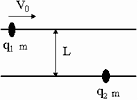
\includegraphics[width=0.45\textwidth]{/faces/group/10}}\\
  \subfloat[Параллель 11 класса.]{\includegraphics[width=0.45\textwidth]{/faces/group/11}}
\end{figure}


\subsection{Преподаватели Летней Физической Школы. }
\label{sec:teachers}

В 1995 году была создана система физического образования в
Санкт-Петербурге, включающая в себя кружки по физике, Летнюю и
Весеннюю физические школы, сборы по подготовке команды СПб к
Всероссийской олимпиаде по физике. Участники кружков, далее победители
олимпиад становились преподавателями, наставниками новых победителей и
успешными учёными. Таким образом, коллектив преподавателей традиционно
состоит из людей, в разное время проходивших обучение в ЛФШ, и
знакомых с традициями преподавания, принятыми в ЛФШ. Важно отметить не
только преподавательскую, но и научную квалификацию исполнителей, что
позволяет осуществлять преподавание на достаточно высоком
содержательном уровне, и заинтересовывать школьников в физике как в
интересной и перспективной профессии.

\textbf{В 8 классе работали:} Н.В.\,Тараканов (преподаватель Городского Центра
Физического Образования), О.В.\,Шустова (студентка 5 курса ФТФ СПбГПУ),
Ф.\,Затылкин (студент 1 курса ФМФ СПбГПУ), В.\,Иванов (студент 1 курса
ФОПФ МФТИ).

\begin{figure}[h]
  \centering
  \subfloat[Н.В.\,Тараканов]{\includegraphics[width=0.2\textwidth]{/faces/maitres/nvtarakanov}}
  \hspace{0.4cm}
  \subfloat[О.В.\,Шустова]{\includegraphics[width=0.2\textwidth]{/faces/maitres/shustova}}
  \hspace{0.4cm}
  \subfloat[Ф.\,Затылкин]{\includegraphics[width=0.2\textwidth]{/faces/maitres/zatylkin}}
  \hspace{0.4cm}
  \subfloat[В.\,Иванов]{\includegraphics[width=0.22\textwidth]{/faces/maitres/ivanov}}
\end{figure}

\textbf{В 9 классе работали:} И.А.\,Барыгин (к.ф.-м.н., педагог дополнительного
образования лицея ФТШ), А.В.\,Лиознова, С.М.\,Атамась (студенты 2 курса
ФТФ СПбГПУ).

\begin{figure}[h]
  \centering
  \centering
  \subfloat[И.А.\,Барыгин]{\includegraphics[width=0.2\textwidth]{/faces/maitres/barygin}}
  \hspace{0.4cm}
  \subfloat[С.М.\,Атамась]{\includegraphics[width=0.2\textwidth]{/faces/maitres/atamas}}
  \hspace{0.4cm}
  \subfloat[А.В.\,Лиознова]{\includegraphics[width=0.2\textwidth]{/faces/maitres/lioznova}}
\end{figure}

\textbf{В 10 классе работали:} С.С.\,Колеватов, А.Г.\,Кострыгин (студенты 4
курса ФФ СПбГУ), Д.С.\,Смирнов (студент 3 курса ФТФ СПбГПУ).

\begin{figure}[h]
  \centering
  \centering
  \subfloat[С.С.\,Колеватов]{\includegraphics[width=0.2\textwidth]{/faces/maitres/sskolevatov}}
  \hspace{0.4cm}
  \subfloat[А.Г.\,Кострыгин]{\includegraphics[width=0.2\textwidth]{/faces/maitres/kostrigin}}
  \hspace{0.4cm}
  \subfloat[Д.С.\,Смирнов]{\includegraphics[width=0.2\textwidth]{/faces/maitres/smirnov}}
\end{figure}


\textbf{В 11 классе работали:} И.Е.\,Шендерович (аспирант ПОМИ
им. В.А.\,Стеклова РАН), Д.В.\,Батькович, Я.Ю.\,Коптелов (студенты 4 курса
ФФ СПбГУ), П.И.\,Буслаев (студент 3 курса ФОПФ МФТИ).

\begin{figure}[h]
  \centering
  \centering
  \subfloat[И.Е.\,Шендерович]{\includegraphics[width=0.2\textwidth]{/faces/maitres/shenderovich}}
  \hspace{0.2cm}
  \subfloat[Д.С.\,Батькович]{\includegraphics[width=0.2\textwidth]{/faces/maitres/batkovich}}
  \hspace{0.2cm}
  \subfloat[Я.Ю.\,Коптелов]{\includegraphics[width=0.2\textwidth]{/faces/maitres/koptelov}}
  \hspace{0.2cm}
  \subfloat[П.И.\,Буслаев]{\includegraphics[width=0.2\textwidth]{/faces/maitres/buslaev}}
\end{figure}

Также в работе школы принимали участие А.В.\,Савельев (к.ф.–м.н.,
доцент УРАН СПб АУ НОЦНТ РАН), А.М.\,Минарский (учитель физики лицея
ФТШ), Р.С.\,Колеватов (к.ф.-м.н., ассистент ФФ СПбГУ), С.Н.\,Тараканов
(психолог).

\begin{figure}[h]
  \centering
  \subfloat[А.В.\,Савельев]{\includegraphics[width=0.2\textwidth]{/faces/maitres/savelyev}}
  \hspace{0.2cm}
  \subfloat[А.М.\,Минарский]{\includegraphics[width=0.2\textwidth]{/faces/maitres/minarsky}}
  \hspace{0.2cm}
  \subfloat[Р.С.\,Колеватов]{\includegraphics[width=0.2\textwidth]{/faces/maitres/rskolevatov}}
\end{figure}

\begin{figure}[h]
  \centering
  \subfloat[С.Н.\,Тараканов]{\includegraphics[width=0.3\textwidth]{/faces/maitres/sntarakanov}}
\end{figure}

Большинство преподавателей в прошлом является победителями олимпиад по
физике, математике и астрономии различных уровней (городских,
Всероссийских и Международных).

\clearpage
\section{Образовательная программа.}
\label{sec:science}

Главное звено в образовательной цепочке ЛФШ~---~\textbf{ежедневные
занятия}. Они проходят каждый день, кроме воскресенья и специальных
дней, отведённых для командных физических соревнований (физбой и
физхоккей). Занятия проходят отдельно для каждого класса
(см. разделы \ref{sec:daily_8}, \ref{sec:daily_9}, \ref{sec:daily_10},
\ref{sec:daily_11}). 

\begin{figure}[h]
  \centering
  \subfloat{\includegraphics[width=0.45\textwidth]{/events/daily08_1}}
  \hspace{0.05\textwidth}
  \subfloat{\includegraphics[width=0.45\textwidth]{/events/daily10_1}}
\end{figure}

В этом году занятия проводились с 9:45 до 13:45. Для удобства
восприятия материала четыре часа занятий были поделены на две
пары. Изначально было запланировано отводить по 105 минут на каждую
пару, но из-за аномально высокой температуры в течение всей смены было
решено сократить пару до 90 минут, а освободившееся время отвести для
купания на озере.

Каждая пара представляла собой теоретическую лекцию, либо решение
задач повышенной сложности, либо выполнение экспериментальной работы с
последующим написанием отчёта. Таким образом, за всю смену в каждой
параллели было прочитано десять лекций, проведено десять занятий по
решению задач, а также выполнено десять экспериментальных работ.

После окончания ежедневных занятий участникам ЛФШ предлагались на
выбор различные \textbf{спецкурсы} (см. раздел
\ref{sec:elective}). Продолжительность этих факультативных занятий
каждый день составляла около двух часов. 

В ЛФШ также имеются мероприятия, проходящие через всю
смену. Во-первых, это \textbf{ежедневные задачи}
(см. \ref{sec:2-a-day}). Каждое утро школьники получают по две задачи
(обычно это задачи из городских олимпиад прошлых лет) для решения и
сдачи преподавателям. Задачи могут сдаваться в течение всей смены. В
качестве стимула для работы в каждом классе был организован <<Экран
задач>>~---~таблица, в которой отмечались успехи каждого школьника. По
итогам смены школьникам, решившим наибольшее количество задач,
выдавался значок <<Лучший теоретик>>.

Во-вторых, это так называемая \textbf{<<Большая Задача>>}
(см. \ref{sec:bz}). По сути, это небольшое исследование на заданную
тему, которое надо провести за время смены. Исследование должно
включать в себя сбор и обработку экспериментальных данных, построение
теории и написание отчёта о проделанной работе. Затем, в один из
вечеров, проводится защита исследования~---~публичное выступление с
результатами работы и дискуссия. Выполнение исследования по <<Большой
Задаче>> проводится в команде из 4-5 школьников. Тем самым, происходит
моделирование реальной научной работы. Члены команды, представившей
лучшее исследование, получают значок <<Лучший исследователь>>.

Кроме этого, в ЛФШ есть два тематических дня, которые проводятся в
первое и второе воскресенье смены --- это \textbf{<<День Изобретателя>>}
(см. \ref{sec:day_inventor}) и \textbf{<<День Экспериментатора>>}
(см. \ref{sec:day_exp}). В <<День Изобретателя>> школьникам
предлагается построить установку, которая обеспечивает заданный эффект
или демонстрирует заданное явление. В <<День Экспериментатора>>
команды школьников соревнуются друг с другом в решении сложных
экспериментальных задач. За победу в этих конкурсах школьники
награждаются значками <<Лучший изобретатель>> и <<Лучший
экспериментатор>>.

Помимо тематических дней, в ЛФШ два дня отводятся под
\textbf{физические бои} (см. \ref{sec:battles}). Члены команды,
победившей в физическом бое, получают значки <<Физбоец>>. В 8-9
классах, помимо физбоя, проводился также \textbf{физический хоккей}.

Ниже приводятся материалы ежедневных занятий, разбитые по классам. 

\subsection{8 класс.}
\label{sec:daily_8}

\subsubsection{Теория.}
\label{sec:daily_8_th}

\textsf{Преподаватель: Н.В.\,Тараканов.}
\smallskip

Курс для 7-8 классов был направлен на то, чтобы сформировать у
учащихся представление о физике, как естественной науке. Показать
единство теоретического и экспериментального подхода, логику
построения научного знания. В рамках теоретического курса обсуждались
вопросы описания механических явлений, а экспериментальная часть была
призвана подкрепить теоретические рассуждения на предметно-чувственном
уровне.

\begin{center}
  \textsf{План занятий.}
\end{center}

\begin{enumerate}
\item Введение. Принципы построения естественных наук. Предмет и
  объект физики.  Постулат существования мира.
\item Пространство и его измерение. Начало отсчета. Определение
  положения тела в пространстве. Декартова система координат и
  полярные координаты.
\item Время и его измерение. Приборы для измерения
  времени. Астрономическое и декретное время.
\item Масса. Понятие массы. Измерение массы тел (гравитационная
  масса). Понятие материальной точки.
\item Характеристики механического движения. Траектория, путь,
  перемещение, скорость.
\item Относительность движения. Системы отсчета. Равномерное
  прямолинейное движение. Первый закон Ньютона.
\item Определение силы. Импульс тела. Второй закон
  Ньютона. Инерциальная масса.
\item Движение тела под действием силы. Ускорение. Равноускоренное
  движение. Перемещение при прямолинейном равноускоренном движении.
\item Причины появления силы. Третий закон Ньютона. Парные силы в
  природе.
\item Трение. Виды трения и их особенности. Разные виды трения в
  природе и технике. Закон Кулона-Амантона.
\item Сила упругости. Деформация тел. Виды деформации. Закон
  Гука. Модуль Юнга.
\item Сила тяжести. Сила тяжести вблизи Земли. Ускорение свободного
  падения тел. Закон Всемирного тяготения. Понятие гравитационного
  поля. Графическое представление полей, силовые линии.
  Характеристики поля. Напряженность силы тяжести.
\item Движение планет. Представление о движении планет в разные
  исторические периоды (Птолемей, Коперник, Браге). Законы Кеплера.
\item Движение тела по окружности. Угловая скорость, период,
  частота. Равномерное движение по окружности. Центростремительная
  сила, центростремительное ускорение. Законы Кеплера, как следствия
  закона Всемирного тяготения.
\end{enumerate}


%%% Local Variables: 
%%% mode: latex
%%% TeX-master: "../../../report"
%%% End: 


\subsubsection{Решение задач.}
\label{sec:daily_8_problems}

\textsf{Преподаватель: О.В.\,Шустова.}
\smallskip
\parindent=0mm

\begin{center}
  \textsf{Листок 1.}
\end{center}
\vspace{0.01mm}
\nopagebreak[2]
\task{ Спортсмен пробегает стометровку за 10 с. Первые 10 м он бежит с
  постоянным ускорением $a$, остальную часть дистанции --- с постоянной
  скоростью $v$. Найдите ускорение $a$ и скорость $v$.  }

\task{ Каретка прибора прошла путь $S$ следующим образом: первую
  половину пути она двигалась с постоянной скоростью $v=12 \unit{м/с}$, вторую
  --- с постоянным отрицательным ускорением так, что в конце пути
  остановилась. Найдите среднюю скорость движения каретки.}

\task{ Ракета стартует с поверхности земли вертикально вверх и в
  течение 10 с поднимается с постоянным ускорением $4{,}9 \unit{м/c}^2$. Затем
  двигатели ракеты отключаются. Найдите максимальную высоту подъема
  ракеты над поверхностью земли. Сопротивлением воздуха
  пренебречь. Ускорение свободного падения считать равным $9{,}8 \unit{м/c}^2$.  }

\task{ Тело свободно падает на землю с некоторой высоты. Начальная
  скорость тела равна нулю. За последнюю секунду оно проходит третью
  часть всего пути. С какой высоты и сколько времени падало тело?
  Сопротивлением воздуха пренебречь. }

\task{ Тело начинает двигаться без начальной скорости с постоянным по
  величине и направлению ускорением $a$. В некоторый момент ускорение
  меняется на противоположное. Найдите путь, пройденный телом за время
  $t_0$ после начала движения, если перемещение тела за время $t_0$ равно
  нулю. }

\begin{center}
  \textsf{Листок 2.}
\end{center}
\vspace{0.01mm}
\nopagebreak[2]
\task{ Машина, трогаясь с места, проходит путь 1 км с постоянным
  ускорением $0{,}2 \unit{м/c}^2$, затем на отрезке пути 1 км ее ускорение равно
  нулю. После этого машина двигается равнозамедленно до полной
  остановки, затратив на эту часть пути время 40 с. Найдите среднюю
  скорость движения машины.}

\task{ Камень бросают вертикально вверх с начальной скоростью 10 м/с с
  высоты 10 м от поверхности земли. Через 1 с после этого с
  поверхности земли вдоль той же самой вертикали бросают вверх другой
  камень с начальной скоростью 20 м/с. Через какое время и на какой
  высоте они столкнутся?  }

\task{ Из точки, находящейся на высоте $x_0$ над землей, одновременно
  бросают два камня с одинаковыми по величине начальными скоростями 10
  м/с --- один вертикально вверх, второй вертикально вниз. Второй камень
  упал на землю через 2 с после броска. На какой высоте над землей
  находится в это время второй камень? Сопротивлением воздуха
  пренебречь.}

\task{ Для определения постоянной скорости судна относительно воды
  производят пробег судна по прямолинейному участку реки между
  пристанями, расположенными на одном берегу на расстоянии 4,2
  км. Время пробега по течению реки 300 с, а против течения 420.
  Какова скорость судна относительно воды? Скорость течения реки
  постоянна на всем участке испытаний.}

\task{ Велосипедист едет по дороге и через каждые 6 секунд проезжает
  мимо столба линии электропередачи. Увеличив скорость на некоторую
  величину $\Delta v$, велосипедист стал проезжать мимо столбов через каждые 4
  секунды. Как часто он будет проезжать мимо столбов, если увеличит
  скорость еще на такую же величину?}

\begin{center}
  \textsf{Листок 3.}
\end{center}
\vspace{0.01mm}
\nopagebreak[2]
\task{ Лодка держит курс перпендикулярно берегу и движется со
  скоростью 7.2 км/ч.  Течение относит ее на расстояние 150 м вниз по
  реке. Найдите скорость течения реки и время, затраченное на переезд
  через реку. Ширина реки равна 0.5 км.}

\task{ Пассажир поезда, идущего со скоростью 40 км/ч, видит в течение
  3 с встречный поезд длиной 75 м. C какой скоростью движется
  встречный поезд?  }

\task{ Дельфин плывет со скоростью 18 км/ч вдоль стенок квадратного
  бассейна, описывая квадрат на постоянном расстоянии от прямолинейных
  участков стенок. За 1 мин он полностью обходит бассейн 3 раза. Найти
  расстояние между дельфином и стенкой. Длина каждой стенки 30 м.}

\task{ Пешеход за первые 20 сек прошел 30 м, за следующие 40 сек ---
  58 м, и за последние 30 сек --- 45 м. Определите скорость движения на
  каждом участке и найдите среднюю скорость за все время движения.  }

\task{ На уроке физкультуры Петя и Маша бежали вместе по прямой
  дорожке, стартовав от школы. Затем, Петя побежал быстрее, а Маша
  пошла. Через некоторое время ребята одновременно повернули обратно и
  достигли школы одновременно. Графики зависимости проекции скорости
  ребят на направление дорожки от времени даны на рисунке. Построить
  графики зависимости расстояния между Петей и Машей от времени.  }

\begin{figure}[h]
  \centering
  \begin{tikzpicture}[>=latex]
    \draw[help lines,step=0.5] (0,-0.5) grid (4,4);
    \draw[thick,->] (0,1.5) -- +(3.7,0) node[above=0.4cm,left=-0.2cm,fill=white] {\footnotesize{$t, \unit{мин}$}};
    \draw[thick,->] (0,-0.5) -- +(0,4.5) node[right,fill=white] {\footnotesize{$V_x, \unit{м/c}$}};
    \draw[very thick,red!50!blue] (0,2.5) -- +(0.5,0);
    \draw[very thick,blue] (0.5,3.5) -- +(1,0);
    \draw[very thick,red] (0.5,2) -- +(1,0);
    \draw[very thick,red!50!blue] (1.5,1.5) -- +(0.5,0);
    \draw[very thick,blue] (2,0) -- +(1.5,0);
    \draw[very thick,red] (2,1) -- +(1.5,0);
    \foreach \x in {1,3,5,7}
    \draw (\x/2,1.6) -- +(0,-0.2) node[anchor=north] {\tiny{$\x$}};
    \foreach \y in {-3.75,-1.25,1.25,2.50,5}
    \draw (-0.1,\y*0.4+1.5) -- +(0.2,0) node[left=0.1cm] {\tiny{$\y$}};
  \end{tikzpicture}
  \label{fig:task_08_15}
\end{figure}

\taskpic{ Двое часовых, двигаясь прямолинейно, охраняют с противоположных
  сторон один небольшой объект. Графики зависимости координат часовых
  от времени даны на рисунке. Постройте: а) графики зависимости скорости в
  часовых от времени б) график зависимости скорости первого часового
  $x$, м относительно второго от времени.}
{
  \begin{tikzpicture}[x=0.8cm,y=0.8cm,>=latex]
    \draw[help lines,step=1] (0,0) grid (4,4);
    \draw[thick,->] (0,-0.2) -- (0,4.5) node[right=0.2cm,fill=white]
    {\footnotesize{$x,\unit{м}$}};
    \draw[thick,->] (0,2) -- (4.6,2) node [above=0.1cm,fill=white] {\footnotesize{$t,\unit{с}$}};
    \foreach \x in {10,20,30}
    \draw (\x/10,2.1) -- +(0,-0.2) node[anchor=north] {\tiny{$\x$}};
    \foreach \y in {-10,10}
    \draw (0,\y/10+2) -- +(0.1,0) node[anchor=west] {\tiny{$\y$}};
    \draw[very thick,red] (0,0) -- (1,1) -- (2,1) -- (3,0) -- (4,2);
    \draw[very thick,blue] (0,4) -- (1,3) -- (2,3) -- (3,4) -- (4,2);
  \end{tikzpicture}
}
\begin{center}
  \textsf{Листок 4.}
\end{center}
\vspace{0.01mm}
\nopagebreak[2] 

\task{ На гладкой горизонтальной поверхности лежат два бруска с
  массами $m_1$ и $m_2$, соединенные невесомой нерастяжимой нитью. Внешняя
  сила $F$ приложена к телу $m_1$ и направлена горизонтально. Найдите
  установившееся ускорение системы и силу натяжения нити.  }

\task{ На горизонтальной поверхности лежат два бруска с массами $m_1$
  и $m_2$, соединенные невесомой нерастяжимой нитью. Внешняя сила $F$
  приложена горизонтально. Определите силу натяжения нити, если
  коэффициенты трения скольжения между поверхностью и брусками равны
  $\mu_1$ и $\mu_2$ соответственно.  }

\task{ Две невесомые пружины имеют длины $l_1$, $l_2$ и жесткости
  $k_1$, $k_2$. Одна пружина вставлена в другую. Концы пружин попарно
  скреплены. Другими точками пружины друг друга не касаются. Какова
  жесткость $k$ получившейся пружины?}

\taskpic{ Система состоит из трех блоков и трех тел массой $m$ каждое,
  связанных невесомыми нерастяжимыми нитями. Масса блока $C$
  пренебрежимо мала. Трение между нитью и блоками отсутствует. Найдите
  ускорения тел. }
{
  \begin{tikzpicture}[interface/.style={postaction={draw,decorate,decoration={border,angle=45,amplitude=0.2cm,segment length=1.5mm}}},>=latex]
  % \draw[help lines,step=0.5] (0,-2) grid (4,4);  
  \draw[very thick,interface] (0.5,4) -- +(3,0);
  \draw[thick] (2,4) -- +(0,-2);
  \draw[very thick] (2,2) circle (1cm);
  \draw[very thick] (2,2) circle (0.25cm);
  \draw[thick] (1,2) -- +(0,-1.5);
  \draw[thick] (3,2) -- +(0,-1.5);
  \draw[very thick] (3-0.75/2,0.5) circle (0.75/2) node[right=0.4cm] {$C$};
  \draw[thick] (3-0.75/2,0.5) -- +(0,-0.75);
  \filldraw[black,thick] (2.75-0.75/2,-0.25) rectangle +(0.5,-0.5)
  node[above right] {$m$};
  \filldraw[black,thick] (0.75,0.5) rectangle +(0.5,-0.5) node[above=0.3cm,left=0.5cm] {$m$};
  \draw[thick] (1.75,2) -- +(0,-2.5);
  \draw[thick] (2.25,2) -- +(0,-1.5);
  \filldraw[black,thick] (1.5,-0.5) rectangle +(0.5,-0.5) node[above=0.3cm,left=0.5cm] {$m$};
\end{tikzpicture}
}
\taskpic{ Два тела с массами $m_1$ и $m_2$ связаны невесомой нерастяжимой
  нитью, перекинутой через невесомый блок, так, что тело $m_2$ висит,
  а тело $m_1$ лежит на горизонтальной поверхности. К телу $m_1$
  приложена в горизонтальном направлении сила $F$. Найдите ускорения
  тел и силу натяжения нити. Трение отсутствует.  }
{
  \begin{tikzpicture}[interface/.style={postaction={draw,decorate,decoration={border,angle=-45,amplitude=0.2cm,segment length=1.5mm}}},>=latex]
  \draw[interface] (0.2,4.5) -- ++(2.5,0) -- ++(0,-3);
  \draw[very thick] (1,4.5) rectangle ++(1,0.75) node[midway] {$m_1$};
  \draw[very thick,->] (1,4.5+0.75/2) -- +(-0.75,0) node[above] {$F$}; 
  \draw[thick] (2.7,4.5) -- ++(0.3,0.3) circle (0.19);
  \draw (2,5) -- ++(1,0) ++(0.19,-0.19) -- +(0,-1.5);
  \draw[very thick] (3.19-0.3,5-0.19-1.5) rectangle ++(0.6,-0.7)
  node[midway] {$m_2$};
\end{tikzpicture}
}

%%% Local Variables: 
%%% mode: latex
%%% TeX-master: "../../../report"
%%% End: 

\begin{center}
  \textsf{Листок 5.}
\end{center}
\vspace{0.01mm}
\nopagebreak[2] 

\task{ Кубик плавает в сосуде с водой так, что его верхняя грань
  параллельна поверхности воды. При этом половина кубика погружена в
  воду. Какой слой масла надо долить, чтобы кубик плавал полностью
  погруженным в жидкость, если плотность масла в два раза меньше
  плотности воды и длина ребра кубика равна $a$? Масло с водой не
  смешивается.  }

\task{ В большом сосуде с водой плавает в вертикальном положении
  тонкостенный стакан, в который налито некоторое количество
  воды. Разность уровней воды в сосуде и стакане равна $x$. Как
  изменится эта разность, если в стакан опустить пробку?  }

\task{ Толстостенная лодка с вертикальными стенками и отверстием в дне
  достаточно долго свободно плавает в озере. Затем отверстие снаружи
  затыкают и внутрь лодки опускают бревно. Повысится или понизится
  после этого уровень воды в лодке относительно уровня воды в озере?}

\task{ Шайба массой $M$, имеющая форму цилиндра с площадью основания
  $S$ и высотой $h$, плавает на границе раздела двух несмешивающихся
  жидкостей с плотностями $\rho_1$ и $\rho_2$ ($\rho_1 <
  \rho_2$). Основание шайбы параллельно границе раздела
  жидкостей. Найдите глубину погружения шайбы в нижнюю жидкость.  }

\setcounter{notask}{1}
\parindent=5mm

\subsubsection{Экспериментальные работы.}
\label{sec:daily_8_exp}

\textsf{Преподаватели: В.\,Иванов, Ф.\,Затылкин.}

Занятия экспериментом в 8 классе были направлены на знакомство с общей
культурой выполнения экспериментальных работ. Школьникам была
прочитана вводная лекция о правилах составления отчётов о проведённых
экспериментальных работах, рассказано о погрешностях. По нашим
наблюдениям, на уроках физики в школе погрешностям уделяется
исключительно мало внимания. Тем не менее, для настоящего понимания
экспериментальной работы необходимо уметь свободно пользоваться этим
аппаратом.

Трудность проведения экспериментальных занятий в 8 классе связана ещё
и с тем, что школьники недостаточно хорошо умеют пользоваться
относительно сложным оборудованием. Поэтому одной из задач было
показать школьникам, что даже с помощью тривиального оборудования
(линейка, монетки, нитки) можно достаточно точно померить различные
физические величины. 

\begin{enumerate}
\item Знакомство с трёхмерной системой координат. 
\item Измерение скорости муравья.  \\ \textit{Оборудование:} линейка,
  секундомер, муравей.
\item Измерение массы капли воды. \\ \textit{Оборудование:} ведро,
  стакан, шприц, монетки.
\item Нахождение центра масс палочки. \\ \textit{Оборудование:}
  линейка, монетки, нитки, палочка.
\item Изучение зависимости силы растяжения резинки от её удлинения. \\
  \textit{Оборудование:} резинка, монетки, линейка.
\item Изучение вращательного движения. \\ \textit{Оборудование:}
  камни, нитки. 
\end{enumerate}


%%% Local Variables: 
%%% mode: latex
%%% TeX-master: "../../../report"
%%% End: 

\subsection{9 класс.}
\label{sec:daily_9}

\subsubsection{Теория.}
\label{sec:daily_9_th}

\textsf{Преподаватель: И.А.\,Барыгин.}
\smallskip

\begin{center}
  \textsf{План занятий.}
\end{center}

\begin{enumerate}
\item Скорость. Радиус-вектор. Мгновенная скорость как предел средней 
скорости. Операции с векторами: сложение, проецирование, скалярное 
произведение.
\item Ускорение. Равноускоренное движение. Скорость и перемещение при 
равноускоренном движении. Движение в однородном поле тяжести: время 
движения, максимальная высота подъема, дальность полета, уравнение 
траектории.
\item Движение по окружности. Период обращения и частота. Угловая 
скорость. Центростремительное ускорение. Нормальное и тангенциальное 
ускорение. Радиус кривизны траектории. Угловое ускорение. Нормальное 
и тангенциальное ускорение при движении с постоянным угловым 
ускорением.
\item Силы. Виды сил. Законы Ньютона. Преобразование координат, 
скоростей и ускорений при переходе в другую систему отсчета. 
\item Закон сохранения импульса. Его связь с третьим законом Ньютона. 
Движение тела с переменной массой.
\item Работа. Кинетическая энергия. Потенциальная энергия. Закон 
сохранения энергии. Потенциальная энергия постоянной силы, силы 
упругости, силы всемирного тяготения.
\item Первый закон Кеплера. Первая и вторая космическая скорость. 
Гравитационный маневр.
\item Центр масс. Второй закон Ньютона для системы тел. Столкновения. 
Рассмотрение абсолютно упругого столкновения в системе отсчета центра 
масс.
\item Правило моментов. Неинерциальные системы отсчета. Сила инерции.
\end{enumerate}


%%% Local Variables: 
%%% mode: latex
%%% TeX-master: "../../../report"
%%% End: 


\subsubsection{Решение задач.}
\label{sec:daily_9_problems}

\textsf{Преподаватель: С.М.\,Атамась.}
\smallskip
\parindent=0mm

\begin{center}
  \textsf{Листок 1.}
\end{center}
\vspace{0.01mm}
\nopagebreak[2]
\task{ Три микрофона, расположенные на одной прямой в точках $А, В,
  С$, зарегистрировали последовательно в моменты времени $t_a > t_b >
  t_c$ звук от взрыва, который произошёл в точке $О$, лежащей на
  отрезке $АС$. Найдите отрезок $АО$, если $АВ=ВС=L$. В какой момент
  времени произошёл взрыв? Скорость звука $c$. }

\task{ По прямому шоссе идёт автобус с постоянной скоростью $V$. Вы
  заметили автобус, когда тот находился в некоторой точке $А$. Из
  какой области около шоссе вы можете догнать автобус если скорость
  вашего бега $V/2$?}

\task{ Сверхзвуковой самолёт летит горизонтально. Два микрофона,
  расположенные на одной вертикали на расстоянии $l$ друг от друга,
  зарегистрировали приход звука от самолёта с запаздыванием времени
  $\Delta t$. Скорость звука в воздухе $c$. Какова скорость самолёта?  }

\task{ По бильярдному столу со сторонами $а$ и $b$ пускают шар из середины
  стороны $b$. Под каким углом к борту стола должен начать движение шар
  чтобы вернуться в ту же точку из которой он начал движение? }
\begin{center}
  \textsf{Листок 2.}
\end{center}
\vspace{0.01mm}
\nopagebreak[2]
\task{ Тело начинает движение из точки $А$ и движется сначала
  равноускоренно в течении времени $t_0$, а затем с тем же по модулю
  ускорением равнозамедленно. Через какое время от начала движения
  тело вернётся в точку $А$?}

\task{ Время отправления электрички по расписанию 12:00. На ваших
  часах 12:00, но мимо вас уже начинает проезжать последний вагон,
  который движется мимо вас в течении 10 с. Последний вагон проходит
  мимо вас за 8 с. Электричка отправилась вовремя, и движется
  равноускоренно. На какое время отстают ваши часы? }

\taskpic{ Из миномёта ведут стрельбу по объектам, расположенным на склоне
  горы. На каком расстоянии от миномёта будут падать мины, если их
  начальная скорость $V$, угол наклона горы $\alpha$ и угол стрельбы по
  отношению к горизонту $\beta$?}{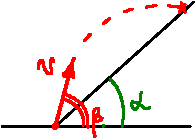
\includegraphics[width=4cm]{p09_7.pdf}}

\taskpic{ Утка летит по горизонтальной прямой с постоянной скоростью $U$. В
  неё бросил камень неопытный охотник, причём в момент броска
  скорость камня $V$ была направлена как раз на утку под углом $\alpha$ к
  горизонту. На какой высоте летела утка, если камень всё же попал в
  неё? }{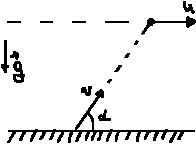
\includegraphics[width=4cm]{p09_8.pdf}}

\begin{center}
  \textsf{Листок 3.}
\end{center}
\vspace{0.01mm}
\nopagebreak[2]
\taskpic{Край гладкого горизонтального стола скруглён по окружности
  радиуса $R$. С какой наименьшей скоростью надо пустить тело, чтобы
  оно, достигнув скругления, сразу полетело по
  пораболе? }{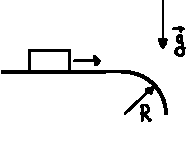
\includegraphics[width=4cm]{p09_9.pdf}}

\taskpic{По деревянным сходням, образующим угол $\alpha$ с горизонтом,
  втаскивают за привязанную к нему верёвку ящик. Коэффициент трения
  ящика о сходни $k$. Под каким углом к горизонту надо тянуть верёвку,
  чтобы с наименьшим усилием втащить ящик? }{
\begin{tikzpicture}[interface/.style={postaction={draw,decorate,decoration={border,angle=-45,amplitude=0.2cm,segment length=1.5mm}}},>=stealth]
   \draw[thick] (0.5,0) -- (3.5,3) -- ++(0,-3) -- cycle;
   \draw[thick,rotate around={45:(1.5,1)}] (1.5,1) rectangle ++(1,0.5);
   \draw[very thick,rotate around={45:(1.5,1)},->] (2.5,1.25) --
   ++(0.7,0.3);
   \draw (1.2,0) arc (0:45:0.7) node[below=0.2cm,right=0.1cm] {$\alpha$};
\end{tikzpicture}
% 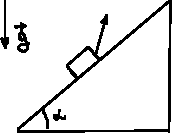
\includegraphics[width=4cm]{p09_10.pdf}
}

\taskpic{Тело массы $m_1$ лежит на доске массы $m_2$, находящейся на гладкой
  горизонтальной поверхности. Коэффициент трения между телом и доской
  $k$. Какую силу надо приложить к доске, чтобы тело соскользнуло с
  неё. За какое время тело соскользнёт, если к доске приложена сила
  $F_0$, а длина доски $l$?  }{
\begin{tikzpicture}[interface/.style={postaction={draw,decorate,decoration={border,angle=-45,amplitude=0.2cm,segment length=1.5mm}}},>=stealth]
%  \draw[help lines,step=0.5] (0,0) grid (4,4);
  \draw[interface] (0.2,0) -- ++(3.2,0);
  \draw[thick] (1,0) rectangle ++(2,0.5) node[midway] {$m_2$};
  \draw[thick] (1,0.5) rectangle ++(1,0.5) node[midway] {$m_1$};
  \draw[very thick,->] (1,0.25) -- ++(-0.5,0) node[above] {$\vec{F}_0$};
\end{tikzpicture}
%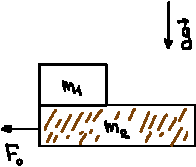
\includegraphics[width=4cm]{p09_11.pdf}
}

\taskpic{Между двумя одинаковыми гладкими брусками массами $m_1$ каждый
  вставлен клин массы $m_2$ с углом $\alpha$. Определите ускорение
  тел. }{
\begin{tikzpicture}[interface/.style={postaction={draw,decorate,decoration={border,angle=-45,amplitude=0.2cm,segment length=1.5mm}}}]
%  \draw[help lines,step=0.5] (0,0) grid (4,4);
  \draw[interface] (0.2,0) -- ++(3.6,0);
  \draw[thick] (0.5,0) rectangle ++(1,1.5) node[midway] {$m_1$}; 
  \draw[thick] (2.5,0) rectangle ++(1,1.5) node[midway] {$m_1$}; 
  \coordinate (a) at ($(1,2.25)!2!(1.5,1.5)$);
  \draw[thick] (1,2.25) -- (a) -- (3,2.25) -- cycle node[below=0.4cm,left=0.5cm]{$m_2$};
  \draw ($(a)!10pt!(3,2.25)$) arc (atan(3/2):90+atan(2/3):10pt)
  node[above=0.25cm,right=-0.05cm] {$\alpha$};
% arc (63:117:0.5) node[above=7,right] {$\alpha$};
\end{tikzpicture}
% %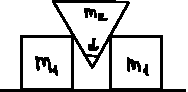
\includegraphics[width=4cm]{p09_12.pdf}
}

\begin{center}
  \textsf{Листок 4.}
\end{center}
\vspace{0.01mm}
\hrule

\task{К свободному концу нити, прикреплённой к стене и перекинутой
  через блок, подвешен груз. Блок закреплён на бруске массы $m_0$,
  который может скользить по горизонтальной плоскости без трения. В
  начальный момент нить с грузом отклоняют от вертикального положения
  на угол $\alpha$ и затем отпускают. Определите ускорение бруска, если
  угол, образованный нитью с вертикалью, не меняется при движении
  системы. Чему равна масса груза.  }

\task{Где находится центр масс: однородного прута, согнутого
  посередине под прямым углом; однородной треугольной пластинки;
  гардеробного номерка в виде диска с круглым отверстием.  }

\task{ Обезьяна массы $m$ уравновешена противовесом на блоке $А$. Блок $А$
  уравновешен грузом массы $2m$ на блоке $В$. Система неподвижна. Как
  будет двигаться груз, если обезьяна начнёт равномерно выбирать
  верёвку со скоростью $V$ относительно себя? Массой блоков и трением
  пренебречь.}

\task{ С какой силой давит на землю кобра, когда она, готовясь к
  прыжку, поднимается вертикально вверх с постоянной скоростью $V$?
  Масса змеи $m$, её длина $l$.  }

\begin{center}
  \textsf{Листок 5.}
\end{center}
\vspace{0.01mm}
\hrule

\task{Автомобиль с работающим д вигателем въезжает на обледенелую
  гору, поверхность которой образует угол $\alpha$ с горизонтом. Какой
  высоты гору может преодолеть автомобиль, если его начальная скорость
  при въезде на него равна $V$, а коэффициент трения колёс о лёд $k$?}

\task{Каков радиус орбиты спутника, лежащей в экваториальной
  плоскости, если тот всё время находится в зените над одной и той же
  точкой земной поверхности?  }

\task{Однородный куб с помощью верёвки, привязанной к середине его
  ребра, подвешен к вертикальной стене. При каких значениях угла
  между верёвкой и стеной куб соприкасается со стеной всей гранью,
  если коэффициент трения его о плоскость равен $k$?}

\task{Лестница опирается на вертикальную стену и пол. При каких
  значениях угла между лестницей и полом она может стоять если
  коэффициент трения лестницы о пол и о стену равен $k_1$ и $k_2$
  соответственно?}

\begin{center}
  \textsf{Листок 6.}
\end{center}
\vspace{0.01mm}
\nopagebreak[2]
\task{Необходимо с поверхности земли попасть камнем в цель, которая
  расположена на высоте $h$ и на расстоянии $S$ по горизонтали. При какой
  наименьшей скорости это возможно? Сопротивлением воздуха пренебречь.}

\task{Между целью и миномётом, находящимся на одной горизонтали,
  расположена стена высотой $h$. Расстояние от стены до миномёта $a$, от
  стены до цели $b$. Определить минимальную начальную скорость мины,
  необходимую для поражения цели. Под каким углом при этом надо
  стрелять? Сопротивлением воздуха пренебречь.  }

\task{Гладкий однородный стержень длины $2L$ опирается на край
  полусферической чаши радиуса $R$. Какой угол с горизонтом образует
  стержень в положении равновесия?}

\task{Зенитное орудие может сообщить снаряду скорость $V$ в любом
  направлении. Требуется найти зону поражения, т. е. границу,
  отделяющую цели, до которых снаряд из данного орудия может долететь,
  от недостижимых целей. Сопротивлением воздуха пренебречь.}

\task{Автомобиль удаляется от стены со скоростью $V$ под углом $\alpha$ к
  ней. В момент, когда расстояние до стены равно $l$, шофёр подаёт
  короткий звуковой сигнал. Какое расстояние пройдёт автомобиль до
  момента, когда шофёр услышит эхо? Скорость звука в воздухе $c$.}

%%% Local Variables: 
%%% mode: latex
%%% TeX-master: "../../../report"
%%% End: 

\begin{center}
  \textsf{Листок 7.}
\end{center}
\vspace{0.01mm}
\nopagebreak[2]

\taskpic{ 
Два одинаковых кубика с длиной ребра $b$ массой $m$ каждый
  стоят на горизонтальном столе, на расстоянии $b$ друг от друга. Между
  ними помещён рычаг длиной $2^{3/2}b$ с пренебрежимо малой
  массой. Коэффициент трения между поверхностями кубиков и столом
  $k$. Коэффициент трения между рычагом и кубиками очень большой в точке
  $A$ и очень маленький в точке $C$. В точке $B$ приложена сила $F$,
  направленная перпендикулярно рычагу как показано на
  рисунке. Определите, какой из кубиков сдвигается раньше, если
  постепенно увеличивать силу $F$.  }
{ 
\begin{tikzpicture}[>=stealth,scale=0.45]
    \draw (-0.4,0) -- (6.4,0);
    \draw[brown,thick] (0,0) rectangle ++(2,2) ++(2,-2) rectangle ++(2,2);
    \coordinate (a) at (2,0);
    \coordinate (f) at ($(a)!5.6!45:(3,0)$);
    \draw[thick] (a) -- (f);
    \draw[->] (f) -- ++(-45:1) node[below] {$\vec{F}$};
  \end{tikzpicture}
%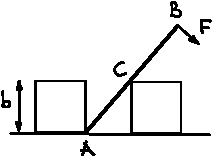
\includegraphics[width=4cm]{p09_26.pdf}
}

\taskpic{ Однородный стрежень длиной $l$ опирается о пол и
  ступеньку. Коэффициент трения между стержнем и полом равен 1, трения
  между стержнем и ступенькой нет. При какой высоте ступеньки стержень
  может находиться в равновесии, если угол $\alpha = \pi /4$?
}{\begin{tikzpicture}[>=stealth,scale=1]
\draw (-0.5,3) -- (0,3) -- (0,0) -- (3.3,0);
\draw[brown, very thick] (3,0) -- +(135:5) node[black,midway, above] {$l$};
\draw[black] (3,0) +(135:0.5) arc (135:180:0.5);
\path (3,0) + (160:0.7) node{$\alpha$};
\draw[thick,->] (2.7,3) -- (2.7,2.5);
\path (3,2.7) node {$\vec{g}$};
\end{tikzpicture}
%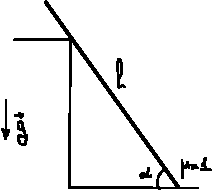
\includegraphics[width=4cm]{p09_27.pdf}
}

\taskpic{ В системе, изображённой на рисунке, трение в блоках и между
  другими поверхностями отсутствует. Если грузу массой $m$ позволить
  двигаться, то за какое время он достигает подставки? Начальная
  скорость груза равна нулю, начальное расстояние от груза до
  подставки $h$, нить невесомая и нерастяжимая. Масса подставки $M$.
}{
\begin{tikzpicture}[>=stealth,scale=0.6]
  \draw (-0.3,0) -- ++(5.3,0) -- ++ (0,5);
  \draw[thick] (0,0) rectangle (2,1) node[midway] {$M$};
  \draw[thick] (0,1) rectangle (1,5);
  \draw (2,0.5) -- (4.6,0.5);
  \filldraw[white,draw=black] (4.6,0.7) circle (0.2);
  \draw (4.6,0.7) -- ++(0.4,-0.3);
  \draw (4.8,0.7) -- ++(0,3.6);
  \filldraw[white,draw=black] (4.6,4.3) circle (0.2);
  \draw (4.6,4.3) -- ++(0.4,0);
  \draw (4.6,4.5) -- ++(-3.2,0);
  \filldraw[white,draw=black] (1.4,4.3) circle (0.2);
  \draw (1.4,4.3) -- ++(-0.4,0.3);
  \draw (1.2,4.3) -- ++(0,-1);
  \draw[thick] (1,3.3) rectangle ++(0.4,-0.4) node[above=0.3cm,right]
  {$m$};
  \draw[dashed] (0,1) -- ++(-0.5,0) ++ (0,2.1) -- ++(1.7,0);
  \draw[thick,<->] (-0.3,1) -- ++(0,2.1) node[midway,left] {$h$};
\end{tikzpicture}
%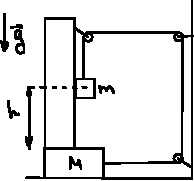
\includegraphics[width=4cm]{p09_28.pdf}
}

\taskpic{ Найдите ускорение грузов, если масса каждого груза равна
  $m$. Массами нитей и блоков пренебречь, нити нерастяжимы, трение
  отсутствует.
}{
\begin{tikzpicture}[scale=0.6]
  \draw (1,0) -- (5,0) (3,0) -- (3,-1.5);
  \filldraw[thick,white,draw=black] (3,-1.5) circle (0.9);
  \draw (2.1,-1.5) -- ++(0,-2) (3.9,-1.5) -- ++(0,-3);
  \filldraw[thick,white,draw=black] (2.1,-3.5) circle (0.6);
  \filldraw[thick,white,draw=black] (3.3,-4.5) circle (0.6);
  \draw (2.7,-3.5) -- +(0,-1);
  \draw (2.1,-3.5) -- +(0,-2.5);
  \draw (3.3,-4.5) -- +(0,-1.5);
  \node [rectangle,fill=white,draw=black,minimum height=0.7,thick] at
  (2.1,-6) {$m$};
  \node [rectangle,fill=white,draw=black,minimum height=0.7,thick] at
  (3.3,-6) {$m$};
\end{tikzpicture}
%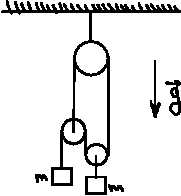
\includegraphics[width=4cm]{p09_29.pdf}
}

\setcounter{notask}{1}
\parindent=5mm

\subsubsection{Экспериментальные работы.}
\label{sec:daily_9_exp}

\textsf{Преподаватель: А.В.\,Лиознова.}

\begin{enumerate}
\item Измерить толщину масляной плёнки. \\ \textit{Оборудование:} шприц, масло, линейка.
\item Найти неизвестное сопротивление. \\ \textit{Оборудование:} вольтметр, батарейка, сопротивление, провода.
\item Измерить силу разрыва нити. \\ \textit{Оборудование:} нитки, кнопки, грузики.
\item Найти показатель преломления жидкости. \\ \textit{Оборудование:} лазерная указка, линейка, бумага, пластиковые стаканчики.
\item Измерить отношение коэффициента трения покоя к коэффициенту
  трения скольжения дерева по дереву. \\ \textit{Оборудование:} деревянный брусок, палочка, линейка.
\item Измерение скорости муравья.  \\ \textit{Оборудование:} линейка,
  секундомер, муравей.
\item Определить содержание соли в воде. \\ \textit{Оборудование:}
  прозрачная бутылка, пластилин, вода с солью, колпачок от ручки.
\item Определить плотность металла в пластилине. \\
  \textit{Оборудование:} разновесы, пластилин с металлом, стакан с
  водой.
\item Исследование времени падения тел различной массы. \\
  \textit{Оборудование:} грузики, секундомер.
\item Нахождение центра масс тела неправильной формы. \\
  \textit{Оборудование:} линейка, нитки, неизвестное тело (вырезано из
  картона).
\end{enumerate}

%%% Local Variables: 
%%% mode: latex
%%% TeX-master: "../../../report"
%%% End: 


\subsection{10 класс.}
\label{sec:daily_10}

\subsubsection{Теория.}
\label{sec:daily_10_th}

\textsf{Преподаватель: С.С.\,Колеватов.}
\smallskip

В 10 классе лекции были посвящены электростатике. Выбор такого
предмета лекций неслучаен: многолетний опыт работы в жюри физических
олимпиад показывает, что школьники зачастую относятся к электростатике
как к набору простейших формул, не понимая физического смысла
явлений. В школьном курсе физики, по нашим наблюдениям, электростатика
была и остаётся одним из самых сложных разделов.

После окончания курса электростатики был прочитан мини–курс по
гидродинамике. Поскольку математический аппарат был довольно схож с
аппаратом электростатики, удалось разобрать довольно большое число
физических явлений, не выводя заново математические факты, а пользуясь
лишь электромеханическими аналогиями. Такой подход, кроме всего
прочего, хорошо демонстрирует единство методов, применяемых в физике. 

\begin{center}
  \textsf{План занятий.}
\end{center}

\begin{enumerate}
\item История.  Закон Кулона. 2 вида зарядов.  Принцип
  суперпозиции. Независимость парных взаимодействий, дискретность
  заряда. Закон сохранения заряда. Напряженность электрического
  поля. Электрическое поле точечного заряда, системы точечных зарядов.
  Линии векторного поля. Поток вектора электрического поля.
  Электростатическая теорема Гаусса и её доказательство.
\item Свойства линий электрического поля. Теорема Ирншоу и её
  доказательство. Задачи на применение теоремы Гаусса.
  Потенциальность кулоновских сил. Электростатические и гравитационные
  силы. Потенциальная энергия. Потенциал. Потенциал точечного заряда.
\item Производная. Частная производная. Градиент. Связь потенциала с
  напряженностью электрического поля. Краевая задача
  электростатики. Задача Дирихле. Задача Неймана. Краевая задача с
  границей в виде проводника.  Проводники. Определение. Свойства
  проводников. Экранирование.
\item Метод изображений. Решение задач с помощью метода изображений.
  Заряд и заземленная плоскость, заземленных уголок, сфера.
  Электростатическая ёмкость уединенного проводника. Ёмкость шара.
\item Ёмкость конденсатора. Плоский конденсатор. Соединение
  конденсаторов. Энергия взаимодействия зарядов. Энергия
  конденсатора. Электрический ток. Плотность тока. Закон
  Ома. Сопротивление. Соединение сопротивлений.
\item Проводимость. Вывод зависимости сопротивления от проводимости и
  размеров тела. Закон Ома в дифференциальной форме. Правила
  Кирхгофа. Алгоритм и пример решения задач. Закон Джоуля-Ленца и его
  доказательство. Сверхпроводники. Высокотемпературная
  сверхпроводимость.
\item Эффект Пельтье. Энергетические уровни. Эффект
  Томсона. Термопара. Градуировка термопары. Решение схем~---~метод
  контурных токов, метод эквивалентной э.д.с.
% \smallskip
% \hrule
\item Гидродинамика. Основные определения. Приближения, в которых
  будут выписываться уравнения. Линии тока, их свойства, связь с
  силовыми линиями. Уравнение неразрывности. Поток через малый
  куб. Запись уравнения аналогично теореме Гаусса. Уравнение Бернулли.
\item Вязкость. Формула Пуазейля (распределение скоростей в
  круглой трубе с жидкостью, поток воды через трубу в единицу
  времени).
\item Вязкость или турбулентность? Коэффициент сопротивления и число
  Рейнольдса. Поверхностное натяжение: поверхностный слой, его
  энергия. Оценка радиуса капли в момент отрыва.

\end{enumerate}


%%% Local Variables: 
%%% mode: latex
%%% TeX-master: "../../../report"
%%% End: 


\subsubsection{Решение задач.}
\label{sec:daily_10_problems}

\textsf{Преподаватель: Д.С.\,Смирнов.}
\smallskip

\begin{center}
  \textsf{Листок 1.}
\end{center}
\vspace{0.01cm}
\nopagebreak[2]
\task{Что будет происходить, если потереть стеклянную палочку о шёлк и
  затем подносить её к бумажному шарику на шёлковой нити? А затем
  коснуться палочкой второго такого же шарика? А затем сблизить
  шарики?}
\task{Как будут меняться показания электроскопа, если трижды коснуться
  его наэлектризованной палочкой?}
\task{Что произойдёт, если соединить два электроскопа: один
  заряженный, а другой нет медной проволокой, держа её в руках? Держа
  её на подвесе из шёлковых нитей? Если соединить те же электроскопы
  чёрной, белой или шёлковой нитью?}
\task{Что будет, если нагреть конец заряженного электроскопа?}
\task{Что будет происходить в последовательном соединении лампочки,
  батарейки и стеклянной трубочки, если последнюю постепенно
  нагревать?}
\task{Что будет, если зарядить один электроскоп стеклянной палочкой
  потёртой о шёлк, другой сургучом потёртым о шерсть, а затем
  соединить их проволокой?}
\task{Как будет вести себя заряженный груз, подвешенный на нити, если
  приближать к нему руку?}

\begin{center}
 \textsf{Листок 2.}
\end{center}
\vspace{0.01cm}
\nopagebreak[2]
\task{Чему равно электрическое поле на оси равномерно заряженной
  сферы, у которой удалили узкий поясок вблизи экватора?}
\task{Сила взаимодействия между двумя одинаковыми зарядами на
  расстоянии 1 м равна 1 Н. Определите эти заряды в СИ и СГС.}
\task{Предположим, что удалось бы разъединить 1 $\mbox{см}^3$ воды на
  элементарные разноимённые заряды, которые затем удалили бы друг от
  друга на расстояние 100 км. С какой силой притягивались бы эти
  заряды?}
\task{На концах горизонтальной трубы длины $l$ закреплены
  положительные заряды $q_1$ и $q_2$. Найдите положение равновесия
  шарика с положительным зарядом $q$, который помещён внутрь
  трубы. Устойчиво ли это положение равновесия? Будет ли положение
  равновесия отрицательно заряженного шарика устойчивым?}
\task{В атоме водорода электрон движется вокруг протона с угловой
  скоростью $10^{16}$ рад/с. Найдите радиус орбиты.}
\task{Чему равна напряжённость электрического поля в центре равномерно
заряженного тонкого кольца радиуса $R$? Чему она равна на оси кольца
на расстоянии $h$ от центра? Заряд кольца $Q$. }
\task{
  Металлическое кольцо разорвалось кулоновскими силами, когда заряд
  кольца был равен $Q$. Сделали точно такое же новое кольцо, но из
  материала, прочность которого в 10 раз больше. Какой заряд разорвёт
  новое кольцо? 
}


%%% Local Variables: 
%%% mode: latex
%%% TeX-master: "../../../report"
%%% End: 

\begin{center}
 \textsf{Листок 3.}
\end{center}
\vspace{0.01cm}
\hrule
\parindent=0mm

\task{
  Напряжённость однородного электрического поля равна $E$. Чему равен
  поток напряжённости электрического поля через квадрат со стороной
  $l$, плоскость которого расположена под углом $30^{o}$ к направлению
  поля? 
}
\task{
  Найдите отрицательные и положительные потоки однородного
  электрического поля напряжённости $E$ через замкнутую поверхность
  прямой трёхгранной призмы, высота которой $h$. Передняя грань
  призмы, ширина которой равна $h$, перпендикулярна $E$, нижняя грань
  параллельна $E$. 
}
\task{Используя теорему Гаусса, определите напряжённость
  электрического поля внутри и вне равномерно заряженной сферы, если
  полный заряд сферы $Q$; равномерно заряженной бесконечной нити, если
  заряд единицы длины равен $\rho$; вне и внутри равномерно заряженной
  бесконечной пластины толщиной $h$, если объёмная плотность заряда в
  пластине равна $\rho$.}
\task{
  Докажите теорему Ирншоу. 
}
\task{
  При пересечении двух шаров радиуса $R$, центры которых находятся на
  расстоянии $l$ друг от друга, образуются два <<полумесяца>>,
  равномерно заряженных разноимёнными электрическими
  зарядами. Объёмная плотность электрического заряда равна
  $\rho$. Докажите, что электрическое поле в области пересечения шаров
  однородно. Найдите его напряжённость. 
}

\taskpic{В равномерно заряженной бесконечной пластине вырезали
  сферическую полость так, как показано на рисунке. Толщина пластины
  $h$, объёмная плотность заряда $\rho$. Чему равна напряжённость
  электрического поля в точке $A$, в точке
  $B$?}{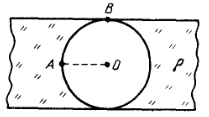
\includegraphics[width=4cm]{d10_3_1.png}}
\task{
  Две пересекающиеся под углом $\alpha$ бесконечные плоскости делят
  пространство на четыре области. Чему равна напряжённость
  электрического поля в этих областях, если поверхностная плотность
  заряда плоскостей $\pm \sigma$?
}
\begin{center}
 \textsf{Листок 4.}
\end{center}
\vspace{0.01cm}
\nopagebreak[2]
\task{Потенциал заряженного проводника 300 В. Какой минимальной
  скоростью должен обладать электрон, чтобы улететь с поверхности
  проводника на бесконечно далёкое от него расстояние?}

\task{
  Заряд 0.1 Кл удалён от заряда 0.2 Кл на расстояние 20 м. Чему равен
  потенциал поля в середине отрезка, соединяющего заряды? 
}

\task{
  Заряды 100, 10, 1, -10, -1, -10 СГС находятся в вершинах правильного
  шестиугольника со стороной 2 см. Чему равен потенциал в центре
  шестиугольника в СИ и СГС? 
}

\task{
  Две бесконечные проводящие изолированные плиты заряжены так, что
  суммарная поверхностная плотность заряда обеих сторон первой плиты
  равна $\sigma_1$, а второй --- $\sigma_2$. Плиты параллельны друг
  другу. Найдите поверхностную плотность заряда на каждой стороне
  плит. 
}

\task{
  Найдите напряжённость электрического поля между тремя пластинами в
  случае, если средняя пластина заземлена. Расстояния между средней
  пластиной и крайними $a$ и $b$. Потенциал крайних пластин $\phi$. 
}

\task{
  В полости металлического шара радиуса $R$ находится заряд
  $Q$. Найдите заряд, индуцируемый этим зарядом на поверхности
  полости. Почему на поверхности шара заряд будет распределён с
  постоянной плотностью? 
}

\task{
  Металлический шар радиуса $R_1$, заряженный до потенциала $\phi$,
  окружают концентрической проводящей незаряженной оболочкой радиуса
  $R_2$. Чему станет равен потенциал шара, если заземлить оболочку?
  Соединить шар с оболочкой проводником? 
}
\begin{center}
 \textsf{Листок 5.}
\end{center}
\vspace{0.01cm}
\hrule
\parindent=0mm

\task{
  Размеры пластин плоского конденсатора увеличили в два раза. Как
  изменилась его ёмкость? Как изменится ёмкость, если расстояние между
  пластинами удвоить? 
}

\task{
  Определите ёмкость конденсатора, образованного двумя
  концентрическими сферами радиуса $R_1$ и $R_2$.
}

\task{
  Определите ёмкость систем конденсаторов, изображённых на рисунке. 
}

\task{
  Как изменится ёмкость плоского конденсатора, если поместить его в
  металлическую коробку? Расстояние от обкладок до стенок коробки
  равно расстоянию между обкладками $d$. Как изменится ёмкость, если
  коробку соединить с одной из обкладок? 
}

\begin{center}
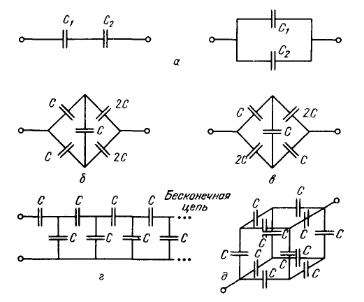
\includegraphics[scale=0.6]{d10_5_1.png}  
\end{center}


\begin{center}
 \textsf{Листок 6.}
\end{center}
\vspace{0.01cm}
\hrule
\parindent=0mm

\task{
  Определите силу, с которой притягиваются друг к другу пластины
  плоского конденсатора, если источник тока, зарядивший конденсатор до
  разности потенциалов 1000 В, отсоединён. Площадь пластин 100
  $\mbox{см}^2$, расстояние между пластинами 1 мм. Изменится ли сила
  взаимодействия пластин, если источник тока будет постоянно
  подсоединён к пластинам?
}

\task{
  Как изменится энергия конденсатора, если при той же разности
  потенциалов между пластинами увеличить все его геометрические размеры
  в $k$ раз?
}

\task{
  На пластины плоского конденсатора помещён заряд $Q$. Площадь пластин
  $S$, расстояние между ними $d$. Какую работу надо совершить, чтобы
  увеличить расстояние между пластинами на $d$? Какую работу надо
  совершить, чтобы сдвинуть пластины на расстояние $x$ относительно
  друг друга? Пластины имеют форму квадрата со сторой $a$. Какая
  совершается работа в обоих предыдущих случаях, если между пластинами
  конденсатора поддерживается батареей постоянная разность
  потенциалов? 
}


\begin{center}
 \textsf{Листок 7 (гидродинамика).}
\end{center}
\vspace{0.01cm}
\nopagebreak[2]
\task{ Под каким углом к горизонту располагается вода в сосуде,
  движущемся с известным ускорением?  }

\task{ Под каким углом к полу вагона расположится чай в стакане, если
  поезд движется по окружности радиусом 1 км со скоростью 72 км/ч ?  }

\task{ С какой скоростью вытекает вода через маленькую дырочку у дна
  широкой бочки с известным уровнем воды? А из узкой бочки, если
  известны площади бочки и дырки? Что изменится, если дырка не в боку,
  а в дне?}

\task{ Как меняется площадь сечения струи, вытекающей из крана, с
  высотой?  }

\task{ Как определить, в какую сторону действует подъёмная сила на
  крыло известной формы? }

\task{ Даны времена, за которые параллелепипедовидная ванна известных
  размеров наполняется из крана и опустошается через дырку в дне. До
  какой высоты дойдёт вода, если одновременно открыть и кран, и дырку?
}

%%% Local Variables: 
%%% mode: latex
%%% TeX-master: "../../../report"
%%% End: 

\begin{center}
 \textsf{Листок 8 (заключительная контрольная).}
\end{center}
\vspace{0.01cm}
\hrule
\parindent=0mm

\task{
  Два одинаковых заряженных шарика массы $m$, подвешенных в одной
  точке на нитях длины $l$, разошлись так, что угол между нитями стал
  прямым. Определите заряд шариков. 
}

\task{Чему равен поток напряжённости однородного электрического
  поля через боковую поверхность усечённого конуса, радиусы сечения
  которого равны $R$ и $r$? Напряжённость электрического поля $E$
  составляет угол $\alpha$ с осью конуса. }

\task{
  Три проводящие концентрические сферы радиуса $r$, $2r$, $3r$ имеют
  заряд соответственно $q$, $2q$, $-3q$. Определите потенциал на
  каждой сфере.
}

\task{ Какие заряды индуцируются на каждом из трёх одинаковых
  конденсаторов ёмкости $C$, соединённых звездой, если подать на
  свободные концы напряжения 0, $\phi$ и $2\phi$?  }

\setcounter{notask}{1}
\setcounter{notask}{1}
\parindent=5mm

\subsubsection{Экспериментальные работы.}
\label{sec:daily_10_exp}

\textsf{Преподаватель: А.Г.\,Кострыгин.}

Экспериментальные занятия в 10 классе были призваны качественно
улучшить имеющуюся у школьников технику проведения экспериментальных
работ. Для этого принципиальные особенности проведения эксперимента
были продемонстрированы на примере распределения Гаусса. Кроме этого,
школьники узнали, что можно экспериментально измерить весьма сложные с
математической точки зрения величины, например, хаусдорфову
размерность природных объектов.

Несколько работ были проведены для того, чтобы продемонстрировать, как
с помощью сравнительно простого оборудования (линейка, секундомер)
можно измерить сложные для прямого измерения величины. 

\begin{enumerate}
\item Измерить модуль упругости каучукового шарика. \\
  \textit{Оборудование:} каучуковый шарик, вода, линейка.
\item Измерить атмосферное давление. \\ \textit{Оборудование:} вода, трубочки, линейка.
\item Распределение Гаусса. \\ \textit{Оборудование:} монетки.
\item Измерение диаметра выходного отверстия у шприца. \\
  \textit{Оборудование:} шприц, линейка.
\item Измерение радиуса песчинки. \\ \textit{Оборудование:}
  секундомер, линейка.
\item Изучение зависимости силы растяжения резинки от её удлинения. \\
  \textit{Оборудование:} миллиметровка, резинка, линейка, грузики.
\item Измерение отношения длин ниток маятника. \\ \textit{Оборудование:} нитки,
  грузики.
\item Нахождение хаусдорфовой размерности листа дерева. \\
  \textit{Оборудование:} лист клёна, линейка.
\item Измерение скорости вытекания воды из крана. \\
  \textit{Оборудование:} линейка.
\item Измерение плотности карандаша. \\ \textit{Оборудование:} вода,
  нитки, линейка, карандаш. 
\end{enumerate}


%%% Local Variables: 
%%% mode: latex
%%% TeX-master: "../../../report"
%%% End: 


\subsection{11 класс.}
\label{sec:daily_11}

\subsubsection{Теория.}
\label{sec:daily_11_th}

\textsf{Преподаватель: И.Е.\,Шендерович.}
\smallskip

В 11 классе лекции были посвящены электродинамике. Последние два
занятия были посвящены применению общей теории к анализу электрических
цепей переменного тока, а также кратко изучалась волновая оптика. 

Целью такого курса было изучение разнообразных методов, широко
применяемых в физике. Кроме того, итогом лекций явилось построение
цельной самосогласованной теории, различные следствия которой можно
наблюдать на эксперименте. Фактически, школьники в первый раз
столкнулись с построением работающей физической теории из
первопринципов (в данном случае за основу были взяты законы
сохранения). 

\begin{center}
  \textsf{План занятий.}
\end{center}

\begin{enumerate}
\item Физические принципы электродинамики. Понятие о физических
  полях. Примеры полей: поле температур, поле скоростей. Скалярные и
  векторные поля. Основные операции с векторами. Начала векторного
  анализа. Интегральные теоремы векторного анализа. Теорема Стокса,
  Гаусса–Остроградского.
\item Электростатика. Закон Кулона как следствие теоремы
  Гаусса. Потенциал как следствие безвихревой природы электрического
  поля. Уравнение Пуассона. Теорема Ирншоу.
\item Энергия электрического поля. Аналогии с гидродинамикой (задача
  об обтекании шара идеальной жидкостью) и теплопроводностью
  (распределение температур в среде с простой геометрией).
\item Сохранение энергии в электродинамике. Связь закона сохранения
  энергии и уравнений Максвелла. Получение уравнений Максвелла, их
  физический смысл. Симметрия в уравнениях Максвелла. Калибровка.
\item Частный случай: магнитостатика. Закон Био–Савара–Лапласа, закон
  Ампера. Примеры применения этих законов, расчёт магнитного поля от
  проводников с током простой формы.
\item Физика индукции. Закон Фарадея. Сила Ампера. Задача про
  взаимодействие параллельных токов. Сила Лоренца. Два источника
  возникновения магнитного поля, физический смысл этого.
\item Движущееся электромагнитное поле. Задача про движущуюся
  заряженную плоскость. Понятие об электромагнитной волне. Волновые
  процессы в электродинамике. Волновое уравнение.
\item Задача про конденсатор в переменном электрическом поле. Пример
  решения физической задачи методом последовательных
  приближений. Функция Бесселя.
\item Законы Кирхгофа. Примеры применения законов Кирхгофа к цепям
  постоянного и переменного тока. Катушки индуктивности. Аналогия с
  механикой. Колебательный контур.
\item Понятие о волновой оптике. Явление интерференции как следствие
  волновой природы света. Интерференция от двух точечных источников
  света. Интерференция на плоскопараллельной пластинке.
\end{enumerate}


%%% Local Variables: 
%%% mode: latex
%%% TeX-master: "../../../report"
%%% End: 


\subsubsection{Решение задач.}
\label{sec:daily_11_problems}

\textsf{Преподаватель: Д.В.\,Батькович.}
\smallskip

\begin{center}
  \textsf{Листок 1.}
\end{center}
\vspace{0.01cm}
\nopagebreak[2]

\taskpic{ На диаграмме изображены два цикла, которые проводят с
  одноатомным идеальным газом: $1-2-3-1$ и $1-3-4-1$. У какого из
  циклов КПД больше и во сколько раз?}{
  \begin{tikzpicture}
    \draw[thick,->] (0,0) -- (0,3.5);
    \draw[thick,->] (0,0) -- (3.5,0);
    \coordinate (a) at (1,1);
    \coordinate (b) at (3,1);
    \coordinate (c) at (3,3);
    \coordinate (d) at (1,3);
    \draw[very thick,red] (a) -- (b) -- (c) -- (a);
    \draw[very thick,red] (a) -- (d) -- (c) -- (a);
    \draw (a) node[below left] {1};
    \draw (b) node[below right] {4};
    \draw (c) node[above right] {3};
    \draw (d) node[above left] {2};
    \draw[blue,dashed] (a) -- ++(0,-1) node[below] {$V$};
    \draw[blue,dashed] (b) -- ++(0,-1) node[below] {$3V$};
    \draw[blue,dashed] (a) -- ++(-1,0) node[left] {$p$};
    \draw[blue,dashed] (d) -- ++(-1,0) node[left] {$2p$};
\end{tikzpicture}  
}

\taskpic{ На расстоянии $d$ от заземленной сферы радиуса $R$ находится
  заряд $q$. Найти потенциал в любой точке пространства.  }{
  \begin{tikzpicture} 
    \draw[very thick] (1,2) circle (1);
    \draw[blue,->] (1,2) --++(100:1) node[midway, left] {$R$};
    \draw[fill=black] (3.5,2) circle (0.05) node[above] {$q$}; 
    \draw[blue,<->] (1,2) -- (3.5,2) node[midway,below] {$d$};
    \draw (1,1) -- (1,0.5);
    \draw (0.75,0.5) -- ++(0.5,0);
    \draw (0.85,0.4) -- ++(0.3,0);
    \draw (0.95,0.3) -- ++(0.1,0);
\end{tikzpicture}  
}

\task{ Планету массой $M$ и радиуса $r$ окружает атмосфера постоянной
  плотности, состоящая из газа с молярной массой $\mu$. Определите
  температуру $T$ атмосферы на поверхности планеты, если толщина
  атмосферы $h$ $(h\ll r)$.  }

\task{ Нелинейный двухполюсник имеет квадратичную ВАХ: напряжение
  между его выводами пропорционально квадрату текущего через него
  тока.  Двухполюсник подключают к батарейке с напряжением $U$
  последовательно с вольтметром, при этом вольтметр показывает
  половину напряжения батарейки. Параллельно двухполюснику подключают
  еще один такой же вольтметр. Найти показания вольтметров. Внутреннее
  сопротивление батарейки считать малым.  }

\task{ Цепь содержит огромное количество звеньев, каждое звено состоит
  из резистора и двух вольтметров. Все вольтметры в цепи
  одинаковы, сопротивления всех резисторов цепи равны между собой.
  Цепь подключают к батарейке, при этом первые два вольтметра
  показывают напряжение $6V$ и $4V$. Найти показания второй пары
  вольтметров. Найти сумму показаний всех вольтметров цепи.  }

\begin{center}
  \begin{circuitikz}
    \draw[thick] (0,2.5) to[battery] (0,0.5) -- (3.5,0.5);
    \draw[thick] (0,2.5) to[generic] (2,2.5) to [voltmeter] (3.5,2.5)
    to[generic] (5.5,2.5) to[voltmeter] (7,2.5) to [voltmeter]
    (7,0.5); 
    \draw[thick] (3.5,2.5) to[voltmeter] (3.5,0.5) to (7,0.5);
    \draw[thick] (7,2.5) -- ++(1,0) node[right] {$\ldots$};
    \draw[thick] (7,0.5) -- ++(1,0) node[right] {$\ldots$};
\end{circuitikz}
\end{center}
\begin{center}
  \textsf{Листок 2.}
\end{center}
\vspace{0.01cm}
\nopagebreak[2]

\task{ В длинной горизонтальной трубе могут скользить без трения два
  поршня, массы которых $M$ и $2M$. Между поршнями находится небольшое
  количество одноатомного идеального газа. Снаружи --- вакуум. В
  начальный момент давление газа $P$, он занимает объем $V$, а поршень
  $M$ имеет скорость $u_{0}$ в направлении второго поршня, который в
  этот момент неподвижен. Найти максимальную скорость тяжелого
  поршня.}

\task{ Вдали от тяготеющих масс в космосе неподвижно висит тонкая
  однородная спица длины $L=10\unit{м}$ и массы $M=1\unit{кг}$. По ней
  может без трения скользить бусинка массы $m=0.1\unit{кг}$. В
  начальный момент бусинка смещена относительно центра спицы на
  $d=1\unit{см}$, система неподвижна.  Через какое время бусинка
  окажется в центре спицы?  Гравитационная постоянная
  $G=6.67 \cdot 10^{-11} \text{ Н}\cdot\text{м}^{2}/\text{кг}^{2}$.}

\task{ На тело, находящееся на горизонтальной шероховатой поверхности
  стола, начинает действовать сила, величина которой возрастает со
  временем по линейному закону. Смещение тела за время $T$, прошедшее
  с момента начала действия силы, составляет $L$, за время $2T$
  смещение равно $50L$. Найти смещение за интервал времени $3T$.  }

\task{ Заряженная частица попадает в среду, где действует сила
  сопротивления, пропорциональная скорости. До полной остановки
  частица проходит путь $S$. Если в среде имеется магнитное поле,
  перпендикулярное скорости частицы, то она при той же начальной
  скорости остановится на расстоянии $L$ от точки входа в среду. На
  каком расстоянии от точки входа в среду остановилась бы частица,
  если бы поле было в два раза меньше? }

\task{ Пластины плоского конденсатора соединены диэлектрической
  пружиной. Начальное расстояние между пластинами $d_{0}$, а после
  того как конденсатор зарядили, оно уменьшилось до величины
  $2d_{0}/2$. Каким будет расстояние между пластинами, если
  параллельно ему подключить такой же конденсатор, но незаряженный.  }

\begin{center}
  \textsf{Листок 3.}
\end{center}
\vspace{0.01cm}
\nopagebreak[2]

\task{ Посередине плоского экрана находится точечный источник света.
  Параллельно экрану расположено плоское зеркало в форме треугольника
  со стороной $a$. Определить площадь зайчика $S$ на экране.  }

\task{ К конденсатору ёмкости $C$ подсоединили резистор сопротивлением
  $R$. Найти зависимость заряда $q(t)$ на резисторе, если в начальный
  момент времени заряд на одной обкладке конденсатора был равен
  $q_{0}$.}

\task{ Найти частоту колебаний $LC$--колебательного контура.  }

\task{ Найти зависимость тока от времени $I(t)$ в $RLC$--контуре, если
  в начальный момент времени заряд на одной обкладке конденсатора был
  равен $q_0$. }

\task{ Из точки А со скоростью $v$ вылетают частицы, имея малый
  разброс $\delta\alpha$, и далее движутся в однородном магнитном поле
  индукции $B$ перпендикулярно ему. Определить, на каком расстоянии от
  точки A соберется пучок, и оцените в этом месте его поперечный
  размер. Масса частиц $m$, заряд $q$. }

\task{ В устройстве для определения изотопного состава ионы калия
  $39K^{+}$ и $41K^{+}$ сначала ускоряются в электрическом поле с
  разностью потенциалов $U$, а затем попадают в однородное магнитное
  поле индукции $B$, перпендикулярное направлению их движения, через
  щель диаметром $d$. Чему должно быть равно $d$, чтобы следы пучков
  на фотопластинке не перекрывались (щель находится в одной плоскости
  с пластинкой). }

\begin{center}
  \textsf{Листок 4.}
\end{center}
\vspace{0.01cm}
\nopagebreak[2]

\task{ Найти период малых колебаний математического маятника с длиной
  подвеса $l$. Ускорение свободного падения равно $g$.  }

\taskpic{ Длинный железнодорожный состав, двигаясь по инерции,
  въезжает на горку с углом наклом $\alpha$. Когда состав
  полностью остановился, на горке находилась половина его
  длины. Сколько времени прошло от начала подъема до остановки? Длина
  состава $L$, трением пренебречь.}{
  \begin{tikzpicture} 
    \draw[very thick] (0,0) -- (2,0) -- (4,1);
    \draw[blue,dashed] (2,0) -- (4,0);
    \draw[blue] (3,0) arc (0:atan(0.5):1);
    \draw[blue] (3.25,0.25) node {$\alpha$};
    \begin{scope}[thick,xshift=-0.2cm]
      \draw (0.5,0.25/2) circle (0.25/2);
      \draw (1,0.25/2) circle (0.25/2);
      \draw (0.3,0.25) rectangle ++(0.9,0.4);
    \end{scope}
    \draw (1,0.4) -- (1.1,0.4);
    \begin{scope}[thick,xshift=0.8cm]
      \draw (0.5,0.25/2) circle (0.25/2);
      \draw (1,0.25/2) circle (0.25/2);
      \draw (0.3,0.25) rectangle ++(0.9,0.4);
    \end{scope}
    \draw (2,0.4) -- (2.22,0.52);
    \begin{scope}[thick,xshift=1.9cm,yshift=0.95cm,rotate around={atan(0.5):(2,0)}]
      \draw (0.5,0.25/2) circle (0.25/2);
      \draw (1,0.25/2) circle (0.25/2);
      \draw (0.3,0.25) rectangle ++(0.9,0.4);
    \end{scope}
    \draw (3,1) -- (3.08,1.04);
    \begin{scope}[thick,xshift=2.8cm,yshift=1.4cm,rotate around={atan(0.5):(2,0)}]
      \draw (0.5,0.25/2) circle (0.25/2);
      \draw (1,0.25/2) circle (0.25/2);
      \draw (0.3,0.25) rectangle ++(0.9,0.4);
    \end{scope}
\end{tikzpicture}  
}

\task{ На очень шероховатый цилиндр радиуса $r$, расположенный
  горизонтально, надет тонкий однородный обруч радиуса $R$. Найти
  период малых колебаний обруча в вертикальной плоскости.}

\task{ Четыре невесомых стержня длины $L$ каждый соединены шарнирно и
образуют ромб $ABCD$. Шарнир $A$ закреплен, а к шарниру $C$ подвешен
груз. Шарниры $D$ и $B$ соединены невесомой пружиной, имеющей в
недеформационном состоянии длину $1.5L$. В положении равновесия
стержни образуют с вертикалью углы $\alpha=30^{\circ}$. Найти период
малых колебаний $T$ системы.}

\taskpic{ Система, изображенная на рисунке, состоит из стержней,
соединенный шарнирно в точках $A$, $B$, $D$, $E$, $G$ и $F$. В точке
$C$ находится бусинка массой $m$. Точки $B$ и $G$, $F$ и $D$
соединены пружинами жесткостью $k$. В положении равновесия все углы
в системе прямые. Найти период малых колебаний системы.}{
\begin{tikzpicture} 
  \draw[interface,thick] (0,0.5) -- (0,3.5);
  \draw[interface,thick] (3.5,3.5) -- (3.5,0.5);
  \draw[very thick] (0,2) node[right] {$A$} -- (3.5/4,3) node[above]
  {$B$} -- (3.5/2,2) node[above=2] {$C$} -- (3*3.5/4,3) node[above]
  {$F$}  --  (3.5,2) node[left] {$E$};
  \draw[very thick] (0,2) -- (3.5/4,1) node [below] {$G$} -- (3.5/2,2)
  node[below=2] {$m$} -- (3*3.5/4,1) node [below] {$D$}--
  (3.5,2);
  \draw[fill=black] (1.75,2) circle (0.1);
  \begin{scope}
    \draw[very thick] (3.5/4,3) -- (3.5/4,2.5);
    \draw[very thick] (3.5/4,1) -- (3.5/4,1.5);
    \draw[very thick,spring] (3.5/4,2.5) -- (3.5/4,1.5);
  \end{scope}
  \begin{scope}[xshift=3.5/2*1cm]
    \draw[very thick] (3.5/4,3) -- (3.5/4,2.5);
    \draw[very thick] (3.5/4,1) -- (3.5/4,1.5);
    \draw[very thick,spring] (3.5/4,2.5) -- (3.5/4,1.5);
  \end{scope}
  \draw[fill=black] (0,2) circle (0.03);
  \draw[fill=black] (3.5,2) circle (0.03);
\end{tikzpicture}  
}
\setcounter{notask}{1}
\parindent=5mm
\newpage
\subsubsection{Экспериментальные работы.}
\label{sec:daily_11_exp}

\textsf{Преподаватель: Я.Ю.\,Коптелов.}
\smallskip

Экспериментальные задачи в 11 классе в большинстве своём состояли из
задач, ранее предлагавшихся на городских и Всероссийских
олимпиадах. Почти в каждой задаче для того, чтобы измерить требуемую
величину с помощью предлагающегося оборудования, школьник должен был
придумать оригинальную методику. Кроме экспериментов по стандартной
школьной программе, в программу 11 класса были включены эксперименты
по интерференции и дифракции (№7, №10), по гидродинамике (№5), а также
по теории колебаний (№9).

\begin{enumerate}
\item Изучение зависимости силы сопротивления среды от скорости. \\
  \textit{Оборудование:} теннисные шарики, нитка, линейка.
\item Изучение распределения вероятностей нахождения груза в
  математическом маятнике. \\ \textit{Оборудование:} нитки, груз.
\item Измерение толщины масляного пятна на поверхности воды. \\
  \textit{Оборудование:} масло, вода, линейка.
\item Измерение массы куска пластилина. \\ \textit{Оборудование:}
  карандаш, вода, нитка, линейка.
\item Измерение радиуса песчинки. \\ \textit{Оборудование:} вода, секундомер.
\item Измерение момента инерции шарика. \\ \textit{Оборудование:}
  каучуковый шарик, вода, линейка.
\item Измерение объёма данных на компакт--диске. \\
  \textit{Оборудование:} компакт--диск, указка, линейка.
\item Измерение плотности карандаша. \\ \textit{Оборудование:} вода,
  нитки, линейка, карандаш.
\item Исследование колебательных мод в двойном маятнике. \\
  \textit{Оборудование:} нитки, монетки.
\item Измерение длины волны лазерной указки. \\ \textit{Оборудование:}
  фольга, булавки, указка, линейка.
\end{enumerate}


%%% Local Variables: 
%%% mode: latex
%%% TeX-master: "../../../report"
%%% End: 

\subsection{Ежедневные задачи.}
\label{sec:2-a-day}

Как уже упоминалось, в начале каждого дня школьники получали по две
задачи для самостоятельного решения. Задачи можно сдавать
преподавателям в течение всей смены. Время для решения и сдачи задач
выбирается школьником самостоятельно. Сдача задач проходит в устной
форме.

Для внесения в процесс решения задач элемента соревнований, в каждом
классе был заведён <<Экран задач>>~---~сводная таблица решённых задач,
обновляющаяся в реальном времени. По окончании смены подводились
итоги: решившим наибольшее количество задач выдавался значок <<Лучший
теоретик>>. 

\subsubsection{Задачи 7 класса.}
\label{sec:2-a-day_7}
\task{Имеется 8~внешне совершенно одинаковых свинцовых шариков, 
однако внутри одного из них сделана небольшая полость. Пользуясь 
только рычажными весами, определите, какой шарик с полостью. Весы 
можно использовать не более двух раз. Опишите свои действия и 
сделайте рисунок.}

\task{Вам даны кастрюля вместимостью 2~л, ведро с водой и чайник, в 
который необходимо как можно точнее отлить из ведра воду объемом 
1~л. Как это можно сделать?}

\task{Вам дана толстая общая тетрадь и линейка. Определите, как 
можно точнее, толщину тетрадного листа.}

\task{Расстояние от Ленинграда до Москвы 650~км, от Ленинграда до 
станции Бологое --- 280~км. Каково расстояние от Москвы до Бологого, 
если все три населенных пункта лежат на одной прямой?}

\task{Имеется 8~внешне совершенно одинаковых восковых шаров, однако 
внутрь одного из них закатана небольшая свинцовая дробинка. 
Пользуясь только рычажными весами, определите, в каком шаре 
находится дробинка. Весы можно использовать не более двух раз. 
Опишите свои действия и сделайте рисунок.}

\taskpic{Легкий воздушный шар и парусная яхта движутся прямолинейно 
равномерно параллельными курсами (в одном направлении). Яхта 
движется в 2~раза медленнее шара. Найдите физическую ошибку на 
рисунке. Сделайте верный рисунок и обоснуйте 
его.}{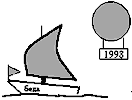
\includegraphics[width=3cm]{d07_06.png}}

\task{Имеются ведро сухого песка, ведро воды и мензурка. Предложите 
способ нахождения объема пустот в ведре сухого песка.}

\taskpic{На пляже имеются два магазина прохладительных напитков. 
Может ли отдыхающий идти так, чтобы к одному магазину он 
приближался, а расстояние до другого оставалось бы постоянным? 
Ответ обоснуйте и сопроводите рисунком. Первоначальное 
положение отдыхающего по отношению к магазинам приведено на 
рисунке (обозначено крестиком).}{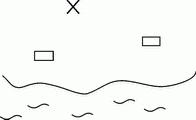
\includegraphics[width=4cm]{d07_08.png}}

\taskpic{Легкий воздушный шар и пароход движутся прямолинейно 
равномерно параллельными курсами (в одном направлении). Шар 
движется в 2~раза быстрее парохода. Найдите физическую ошибку на 
рисунке. Сделайте верный рисунок и обоснуйте 
его.}{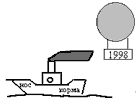
\includegraphics[width=3cm]{d07_09.png}}

\task{Три лучника стоят на одной линии на расстоянии 2~м друг от 
друга и стреляют последовательно через 1~с перпендикулярно линии 
стрельбы по длинной мишени, которая движется параллельно линии 
стрельбы со скоростью 0{,}5~м/с. На каком расстоянии друг от друга 
попадут стрелы в мишень, если известно, что все они летят с 
одинаковыми скоростями?}

\taskpic{В залив впадают два ручья. Можно ли на лодке двигаться по 
заливу так, чтобы, удаляясь от устья одного ручья, оставаться на 
постоянном расстоянии от устья другого? Ответ обоснуйте и 
сопроводите рисунком. Первоначальное расположение лодки по 
отношению к ручьям приведено на рисунке.}{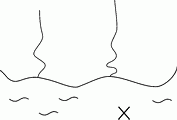
\includegraphics[width=4cm]{d07_11.png}}

\task{Плот плывет по течению реки в южном направлении. На плоту 
сидит мальчик и ловит рыбу. В какую сторону от положения 
вертикали будет отклоняться леска (и будет ли) находящаяся под 
водой?}

\task{В тире четыре стрелка, стоя на одной линии, стреляют в 
движущуюся мишень. На каком расстоянии будут следы от пуль на 
мишени, если она движется со скоростью 0{,}5~м/с параллельно линии 
стрельбы; стрелки стоят на расстоянии 1~м друг от друга и стреляют 
последовательно через 1~с?}

\task{Воздушный шар уносится ветром в северо-восточном 
направлении. В какую сторону будут развеваться флаги, украшающие 
шар?}

\task{Трем туристам необходимо за максимально короткий срок 
добраться из одного населенного пункта в другой. Как это сделать, 
если у них имеется лишь один одноместный велосипед? Скорость 
пешехода в 2 раза меньше велосипедиста. Построить график 
зависимость пройденного пути от времени для всех тел, 
участвующих в движении.}

\task{У Вас есть моток тонкой проволоки, карандаш и тетрадь в 
клетку. Как можно определить диаметр поперечного сечения 
проволоки?}

\task{Имеются ведро сухого песка, ведро воды и мензурка. Предложите 
способ нахождения объема пустот в ведре сухого песка.}

\task{За сутки молодой бамбук может вырасти на 86,4 см. На сколько он 
вырастает за секунду?}

\task{На какой угол поворачивается Земля вокруг своей оси за 1~мин?}

\task{Сколько потребовалось бы времени для того, чтобы уложить в 
ряд кубики, объемом 1~мм$^3$ каждый, взятые в таком количестве, 
сколько содержится их в 1~м$^3$ , если на укладку одного кубика 
затрачивается время, равное 1~с?}

\task{Четыре мальчика отправились из одного населенного пункта в 
другой, имея лишь один одноместный велосипед. Известно, что 
скорость велосипедиста в 4~раза больше скорости пешехода. Что 
необходимо сделать, чтобы как можно быстрее проделать этот путь? 
Построить график зависимости пройденного пути от времени для 
всех тел, участвующих в движении.}

\task{Мальчик идет из дома в школу, расстояние от дома до которой 
1200~м. Он всегда приходил в школу в одно и то же время. Но на трети 
пути он вспоминает, что забыл дневник, и решает вернуться домой 
за дневником. С какой скоростью он должен бежать с этого момента , 
чтобы успеть в школу в то же время, если обычно он идет с 
постоянной скоростью 7{,}2~км/ч?}

\task{Имеются ведро сухого песка, ведро воды и мензурка. Предложите 
способ нахождения собственного объема песчинок в ведре сухого 
песка.}

\taskpic{Во время археологических раскопок была найдена старинная 
бутылка, нижняя часть которой имеет форму параллелепипеда и по 
объему составляет около $\frac{2}{3}$ от всей бутылки. Верхняя часть 
бутылки имеет неправильную форму. Имея в распоряжении линейку, 
пробку к этой бутылке и неограниченные запасы воды, определите 
объем этой бутылки.}{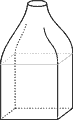
\includegraphics[width=1.5cm]{d07_24.png}}

\task{Почему при резком торможении передним колесом велосипеда 
есть опасность перелететь через руль?}

\taskpic{Вода вытекает с постоянной скоростью $v$ из двух одинаковых 
труб в одну трубу с площадью поперечного сечения в 3~раза большей, 
чем у каждой из двух предыдущих труб. Какова скорость $u$ течения 
воды в трубе большого сечения? Вода полностью заполняет 
трубы.}{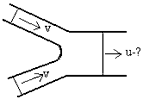
\includegraphics[width=3cm]{d07_26.png}}

\task{Имеются рычажные весы с чашами различной массы, набор 
одинаковых кубиков, набор одинаковых шариков. Весы находятся в 
равновесии, если положить: на левую чашу 2~кубика, на правую 
3~шарика; или на левую чашу 1~шарик, на правую 1~кубик. Какая чаша 
весов опустится, если положить: на левую чашу 1~кубик, на правую 
1~шарик? Ответ обоснуйте.}

\task{На одной из линий метрополитена все станции расположены на 
одинаковом расстоянии. На преодоление этого расстояния поезд 
метро тратит 4~минуты. В каждую сторону поезда ходят один раз в 
3~минуты. На одной из станций машинист заметил, что на 
противоположной платформе стоит поезд. Через какое время он 
снова увидит поезд, следующий в противоположную сторону?}

\task{На линии метро расположено 10~станций на одинаковом 
расстоянии друг от друга. Между соседними станциями поезд 
движется 3~минуты. Линию обслуживают 18~поездов. К очередному 
празднику было решено ввести новую конечную станцию. Её 
расположили так, что время движения от неё до ближайшей станции 
метро составило 6~минут. На всех станциях поезд проводит 3~минуты. 
На конечных станциях поезд также стоит 3~минуты, после чего едет в 
обратном направлении. Сколько нужно ввести дополнительных 
поездов, чтобы интервал между их появлениями (в одном 
направлении) на станциях остался прежним?}

\task{С территории военной части Х, расположенной вблизи города Y, 
одновременно выехали три танка. Ехали они по одной дороге, и 
скорость каждого из них была постоянна. Скорость первого танка 
равнялась $v_1 = 30\mbox{ км/ч}$, скорость второго $v_2 = 20\mbox{ км/ч}$. Первый 
танк въехал в город Y в 19{.}00, второй танк --- в 20{.}00, а третий танк --- в 
21{.}00. Найдите скорость третьего танка.}

\setcounter{notask}{1}
\vspace{1cm}

\begin{center}
\textbf{Лучшие теоретики:}
\end{center}

\begin{figure}[h]
  \centering
  \subfloat[Андрей Йона]{\includegraphics[height=6cm]{/faces/best_th/iona}}
  \hspace{0.05\textwidth}
  \subfloat[Павел Ходунов]{\includegraphics[height=6cm]{/faces/best_th/pkhodunov}}
\end{figure}

\subsubsection{Задачи 8 класса.}
\label{sec:2-a-day_8}
\task{Имеется 8~внешне совершенно одинаковых свинцовых шариков, 
однако внутри одного из них сделана небольшая полость. Пользуясь 
только рычажными весами, определите, какой шарик с полостью. Весы 
можно использовать не более двух раз. Опишите свои действия и 
сделайте рисунок.}

\task{Два друга, Петр и Павел, поехали на поезде. У Петра был билет в 
первый вагон, а у Павла --- в последний (вагоны нумеруются от 
локомотива). На одной из промежуточных остановок локомотив 
перецепили к хвосту поезда, поэтому Петр приехал в конечный 
пункт в последнем вагоне, а Павел --- в первом. Сравните пути 
вагонов, в которых ехали Петр и Павел.}

\task{Заводной игрушечный автомобиль едет по полу. В кузове 
автомобиля стоит оловянный солдатик. Автомобиль сталкивается со 
стенкой. В каком направлении по отношению к направлению движения 
автомобиля упадет солдатик? Ответ обоснуйте.}

\task{Имеется чайник с водой, нить, мензурка и тело неправильной 
формы, не входящее в мензурку.  Как можно определить объем этого 
тела? Опишите и сделайте рисунок.}

\task{Эскалатор одной из станций метро поднимает неподвижно 
стоящего на нем пассажира в течение 2~мин. По неподвижному 
эскалатору пассажир поднимается в течение 6~мин. Сколько времени 
будет подниматься пассажир идущий вверх по движущемуся 
эскалатору?}

\task{С лодки, идущей вниз по течению реки, уронили в воду весло. 
Через час после этого решили подобрать весло и повернули 
обратно. Через какое время лодка повстречает весло, если 
скорость течения одинакова по всей реке, а мотор лодки все время 
работает в одинаковом режиме?}

\task{Пеностекло получают вспениванием стекла в процессе варки, 
вводя пенообразующее вещество. Сколько процентов объема 
пеностекла занимают газы, массой которых можно пренебречь, если 
плотность пеностекла $\rho_1 = 200\mbox{ кг/м}^3$? Плотность обычного 
стекла $\rho_0 = 2500\mbox{ кг/м}^3$.}

\taskpic{В изогнутую трубку наливают воду до тех пор, пока она не 
начинает переливаться через край. Широкое колено закрывают 
крышкой массой $M$. Какую массу воды нужно долить, чтобы крышка 
поднялась? Площадь широкого колена $S_1$, площадь узкого колена 
$S_2$.}{
\begin{tikzpicture}
  \draw[thick,fill=blue!20] (3.5,3) -- (3.5,0) -- (0.5,0) --
  (0.5,2) -- (1.5,2) -- (1.5,0.5) -- (3,0.5) -- (3,3);
  \draw[pattern=north east lines] (0.4,2) rectangle ++(1.2,0.3);
  \draw (1,1.7) node {$S_1$};
  \draw (3.25,3.25) node {$S_2$};
\end{tikzpicture}  
}

\task{Идет дождь. Капли падают вертикально со скоростью $v$. 
Неподвижное цилиндрическое ведро с площадью дна $S$ наполняется 
со скоростью 1~кг/мин. Самолет летит горизонтально со скоростью 
$4v$. Какая масса воды попадает за минуту в цилиндрический 
воздухозаборник самолета площадью $2S$?}%{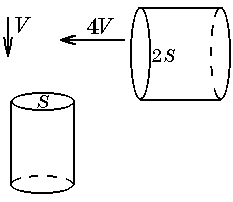
\includegraphics[width=4cm]{d08_09.png}}

\task{Судно выходит из реки в море. Как при этом изменяется 
архимедова сила, действующая на судно? Ответ обоснуйте.}

\task{Оцените массу атмосферы Венеры. Венеру считать шаром с 
площадью поверхности $4{,}7\cdot10^{14}\mbox{ м}^2$. Величина $g$ для Венеры 
равна 8{,}7~Н/кг. Атмосферное давление у поверхности Венеры 9120~кПа.}

\task{Тело подвешено на пружине динамометра. При взвешивании тела в 
пустоте показание динамометра $P$. При взвешивании этого же тела в 
жидкости плотностью $\rho_1$ динамометр показывает $P_1$. Какова 
плотность тела? При взвешивании тело полностью погружается в 
жидкость и не растворяется в ней.}

\task{Катер плывет по реке против течения с постоянной скоростью и 
в некотором определенном месте теряет спасательный круг. Через 
время $t$ потеря обнаруживается, катер поворачивает обратно и 
нагоняет круг на расстоянии $S$ ниже места потери. Какова скорость 
течения реки, если мотор катера при движении против течения и по 
течению работает в одинаковом режиме?}

\task{Тело подвешено на пружине динамометра. При взвешивании тела в 
пустоте показания динамометра $P$. При взвешивании этого же тела в 
жидкости с плотностью $\rho_1$ динамометр показывает $P_1$. При 
взвешивании тела в жидкости с неизвестной плотностью $\rho_2$ 
динамометр показывает $P_2$. Какова плотность жидкости $\rho_2$? При 
взвешивании тело полностью погружается в обе жидкости и не 
растворяется в них.}

\task{Из города А выехала автомашина, движущаяся со скоростью 10~м/с, 
и одновременно навстречу ей из города В выехал велосипедист, 
движущийся со скоростью 18~км/ч. Расстояние между городами 108~км 
(путь прямой). Постройте график зависимости пройденного пути от 
времени для каждой машины и по этим графикам определите 
пройденные пути и время движения автомашины и велосипедиста до 
их встречи.}

\task{В сосуде с водой плавает шар, наполовину погрузившись в воду. 
Изменится ли глубина погружения шара, если этот сосуд с шаром 
перенести на планету, где сила тяжести в два раза больше, чем на 
Земле?}

\task{Мальчик проплыл на надувной лодке по реке вниз и вверх по 
течению, а затем, прилагая те же усилия к той же лодке, проделал 
такой же длины путь по озеру со стоячей водой. В котором случае 
мальчик расходовал меньше времени, проплывая намеченный им путь?}

\task{Ко дну сосуда с водой приморожен шарик из льда. Как изменится 
уровень воды в сосуде, когда лед растает? Изменится ли при этом 
сила давления воды на дно сосуда?}

\task{Для барометра мальчики сделали барометрическую трубку, в 
которой средняя часть (в несколько сантиметров длиной) 
представляет трубку из эластичной резины. Как под действием 
ртути в такой составной трубке их барометра была деформирована 
резиновая часть трубки --- сузилась или расширилась?}

\task{В сосуде с водой плавает кусок льда. Изменится ли уровень воды 
в сосуде, если лед растает?}

\task{Теплоход движется со скоростью 18~км/ч. По его палубе от кормы 
до носовой части и обратно идет пассажир со скоростью 3{,}6~км/ч 
относительно теплохода. Какой путь относительно берега пройдет 
пассажир, если длина теплохода 100~м?}

\task{В сосуде с водой плавает кусок льда, в котором находится 
пузырек воздуха. Изменится ли уровень воды в сосуде, когда лед 
растает?}

\task{Первую треть пути мотоциклист проехал со скоростью 40~км/ч, 
остальной путь --- 50~км/ч. Определите среднюю скорость движения на 
всем пути.}

\task{В сосуде с водой плавает кусок льда с вмерзшим в него стальным 
шариком. Изменится ли уровень воды в сосуде, когда лед растает?}

\task{В цилиндрический сосуд с площадью основания $S = 100\mbox{ см}^2$ 
налит 1~литр соленой воды плотности $\rho_1 = 1{,}15\mbox{ г/см}^3$. В этой 
воде плавает кусок льда из пресной воды массой $m = 1\mbox{ кг}$. 
Определите, как изменится уровень воды в сосуде, если половина 
льда растает. Считать, что при растворении соли в воде объем 
жидкости не изменяется.}

\task{В сосуде с водой на подставках находится цилиндр без дна. 
Высота выступающей из воды части цилиндра равна $h = 5\mbox{ см}$. 
Какую высоту должен иметь цилиндр, чтобы его можно было 
заполнить маслом целиком?}

\task{В сосуде с водой плавает брусок из льда, на котором лежит 
деревянный шар. Плотность вещества шара меньше плотности воды. 
Изменится ли уровень воды в сосуде, если лед растает?}

\task{Вагон поезда, движущегося со скоростью 36~км/ч, был пробит 
пулей, летевшей перпендикулярно к движению поезда. Одно 
отверстие в стенках вагона смещено относительно другого на 3~см. 
Ширина вагона --- 2{,}7~м. Какова скорость движения пули?}

\task{Когда мимо пристани проходил плот, в деревню, находящуюся на 
расстоянии 15~км от пристани, вниз по реке отправилась моторная 
лодка. Она дошла до деревни за $\frac{3}{4}$ часа и, повернув обратно, 
встретила плот на расстоянии 9~км от деревни. Какова скорость 
течения реки и скорость лодки относительно воды?}

\task{На чашке весов стоит стакан с водой. Изменятся ли показания 
весов, если в воду погрузить гирю, подвешенную на нити к штативу?}

\task{Большой круг установлен в центре прямоугольного зала на 
уровне пола и равномерно вращается. Мальчик, часто подпрыгивая 
на одной ноге, пересекает круг в направлении диагонали зала. При 
этом на круге остается след ступни мальчика. Сплошной линией 
покажите траекторию движения мальчика относительно круга. 
Скорость мальчика (относительно земли) считать такой, что за то 
время, пока круг делает половину оборота, мальчик преодолевает 
путь, равный длине диаметра круга.}

\taskpic{На равноплечных весах уравновешены два одинаковых 
цилиндрических сосуда с водой. Уровни воды в обоих сосудах 
совпадают. В сосуд опускают одинаковые шары объема $V$ массы $M$ 
каждый, плотности которых меньше плотности воды. В левый сосуд 
шар опускают на жесткой штанге, к концу которой он привязан с 
помощью нити. В правый сосуд шар опускают на нити, перекинутой 
через неподвижный блок. Оба шара полностью погружены в воду. 
Какой груз и на какую чашку надо добавить, чтобы не нарушилось 
равновесие? Объемами штанги, нити, блока пренебречь. Плотность 
воды считать известной.}{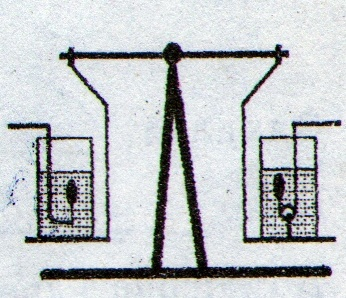
\includegraphics[width=4cm]{d08_32.jpg}}

\task{На тренировке по баскетболу два спортсмена выполняют 
передачи мяча, непрерывно двигаясь навстречу друг другу. Сколько 
передач они успеют сделать до того момента, когда пробегут мимо 
друг друга, если скорости движения спортсменов постоянны и равны 
1~м/с, скорость полета мяча --- 10~м/с, время, затрачиваемое на каждый 
прием и передачу --- 0{,}2~с. Начальное расстояние между 
баскетболистами --- 10~м.}

\task{Толстостенная лодка с вертикальными стенками и отверстием в 
дне достаточно долго свободно плавает в озере. Затем отверстие 
затыкают и потом внутрь лодки пускают плавать бревно. Повысится 
или понизится после этого уровень воды в лодке относительно 
уровня воды в озере?}

\task{Наблюдая за равномерно движущимся поездом, мальчик 
определил, что мимо начала железнодорожной платформы поезд 
двигался в течение времени $t_1 = 23\mbox{ c}$. Одновременно с этим его 
приятель установил, что мимо этой платформы поезд двигался в 
течение времени $t_2 = 39\mbox{ c}$. Измерив длину платформы, которая 
оказалась равной $l = 240\mbox{ м}$, мальчики определили скорость и 
длину поезда. Какие числовые значения этих физических величин 
получили мальчики?}

\task{В сосуде с водой плавает железный коробок, ко дну которого при 
помощи нити подвешен стальной шар. Шар не касается дна сосуда. 
Как изменится высота уровня воды в сосуде, если нить, 
удерживающая шар, оборвется?}

\setcounter{notask}{1}
\vspace{1cm}

\begin{center}
  \textbf{Лучшие теоретики:}
\end{center}

\begin{figure}[h]
  \centering
  \subfloat[Софья Коско]{\includegraphics[height=6cm]{/faces/best_th/kosko}}
  \hspace{0.05\textwidth}
  \subfloat[Мария Муретова]{\includegraphics[height=6cm]{/faces/best_th/muretova}}
\end{figure}

\subsubsection{Задачи 9 класса.}
\label{sec:2-a-day_9}
\task{ В комнате на столе в патронах стоят 3~лампочки. Снаружи у 
двери комнаты имеются три выключателя, каждым из которых можно 
включить только одну лампочку. Определите каким ключом 
включается каждая лампочка, если открыть дверь и войти в комнату 
можно только один раз. Опишите свои действия. }

\task{ Тело подвешено на пружине динамометра.  При взвешивании тела 
в пустоте показания динамометра $P$.  При взвешивании этого же 
тела в жидкости с плотностью $\rho_1$ динамометр показывает $P_1$. При 
взвешивании тела в жидкости с неизвестной плотностью $\rho_2$ 
динамометр показывает $P_2$. Какова плотность жидкости $\rho_2$? При 
взвешивании тело полностью погружается в обе жидкости и не 
растворяется в них. }

\taskpic{ Груз весом $P$ подвешен на невесомом шарнире с тремя 
звеньями. Определите силу натяжения нити, соединяющей точки 
шарнира А и В. }{
\begin{tikzpicture}
  \draw[interface,thick] (1.25,3.5) -- (2.75,3.5);
  \draw[thick] (2,3.5) -- (2,3);
  \begin{scope}
    \draw[thick] (1.75,3.25) -- ++(0.25,0.25) -- ++(0.25,-0.25);
    \draw[thick] (1.75,3.25) -- ++(0.25,-0.25) -- ++(0.25,0.25);
  \end{scope}
  \begin{scope}[yshift=-0.5cm]
    \draw[thick] (1.75,3.25) -- ++(0.25,0.25) -- ++(0.25,-0.25);
    \draw[thick] (1.75,3.25) -- ++(0.25,-0.25) -- ++(0.25,0.25);
  \end{scope}
  \begin{scope}[yshift=-1cm]
    \draw[thick] (1.75,3.25) -- ++(0.25,0.25) -- ++(0.25,-0.25);
    \draw[thick] (1.75,3.25) -- ++(0.25,-0.25) -- ++(0.25,0.25);
  \end{scope}
  \draw (2,2) -- (2,1.75);
  \draw[fill=black] (1.75,1.75) rectangle ++(0.5,-0.5);
  \draw[blue,->] (2.6,3) node[right,black] {\tiny{$A$}} to[out=180,in=-20] (2.15,3.45);
  \draw[blue,->] (2.6,2.5) node[right,black] {\tiny{$B$}} to[out=180,in=-20] (2.15,2.95);
\end{tikzpicture}  
}

\task{ Сколько времени потребуется для превращения 2~л воды, взятой 
при температуре 20$^\circ$C в пар с температурой 100$^\circ$C? Нагревание 
происходит на горелке, расходующей 0{,}69~кг керосина в час. 
Теплоемкостью сосуда, в котором находится вода, пренебречь. 
Считать, что все тепло при сгорании керосина подводится к воде. 
Удельная теплота сгорания керосина $q = 4{,}6\cdot 10^7$~Дж/кг, удельная 
теплоемкость воды $c=4{,}2\cdot 10^3$~Дж/(кг$\cdot^\circ$C), удельная теплота 
парообразования воды $L=2{,}3\cdot10^6$~Дж/кг. }

\task{ Оцените массу атмосферы Венеры. Венеру считать шаром с 
площадью поверхности $4{,}7\cdot10^{14}$~м$^2$. Величина $g$ для Венеры равна 
  $8{,}7$~Н/кг. Атмосферное давление у поверхности Венеры 9120~кПа. }

\taskpic{ Два одинаковых проводника, изготовленных так, что их 
удельное сопротивление линейно изменяется с расстоянием от 
начала проводника: $\rho = kL$, где $\rho$ --- удельное сопротивление 
проводника, $k$ --- известный постоянный коэффициент,  $L$ --- 
расстояние от начала проводника до данной точки, соединены 
параллельно так, что у одного удельное сопротивление возрастает 
справа налево, а у другого наоборот --- слева направо. Эта схема 
подключена к источнику постоянного тока с напряжением $U_0$ 
(см.рис.). Какое напряжение показывает идеальный вольтметр, 
соединяющий середины этих проводников? }{
\begin{circuitikz}
  \draw[o-,thick] (1.5,0.5) -- (0.5,0.5) -- (0.5,3.5);
  \draw[thick] (0.5,3.5) to[generic] (3.5,3.5) -- (3.5,1.5)
  to[generic] (0.5,1.5);
  \draw[o-,thick] (2.5,0.5) -- (3.5,0.5) -- (3.5,1.5);
  \draw[thick] (2,3.25) to[voltmeter] (2,1.75);
  \draw (2,0.5) node {$U_0$};
\end{circuitikz}
}

\task{ По прямому участку железнодорожного пути движется вагон со 
скоростью 14{,}4~км/ч. В вагоне мальчик пускает игрушечный состав по 
рельсам, расположенным поперек вагона. Скорость состава 
относительно пола вагона равна 3~м/с. Найти скорость игрушечного 
состава относительно Земли. }

\task{ Том вплотную подобрался к Джерри, двигаясь с постоянной 
скоростью $v$. В этот момент Джерри начинает убегать от Тома, 
двигаясь по прямой со скоростью $u$ = $k/R$, где $R$ --- расстояние между 
котом и мышью, $k$ --- постоянный независимый коэффициент. Найти 
установившееся расстояние между ними. }

\taskpic{ Из четырех нихромовых проволочек с удельным 
сопротивлением $\rho$, площадью сечения $S$, длиной $L$ каждая, 
выполнена фигура, представляющая собой крест. Крест подключают к 
источнику постоянного тока напряжением $U$, как показано на 
рисунке (положительный полюс к точке пересечения проволочек, 
отрицательный полюс к концам креста). Фигуру помещают в термос с 
дистиллированной водой. В некоторый момент времени  замыкают 
ключ. Вода закипела через время $\Delta t$. Сколько воды находилось в 
термосе? Удельная теплоемкость воды $c$, начальная температура $T$.  
Потерями тепла пренебречь. }{
\begin{tikzpicture}
  \draw[blue] (0.75,1.5) to[out=45] (2,2.5);
  \draw[red] (0,1.5) to[out=90,in=90] (2.5,2.5);
  \draw[red] (0.75,2.25) to[out=90] (2.5,2.5);
  \draw[red] (1.5,1.5) to[out=20,in=-100] (2.5,2.5);
  \draw[red] (0.75,0.75) to[out=-20,in=-100] (2.5,2.5);
  \draw[very thick] (0,1.5) -- (1.5,1.5);
  \draw[very thick] (0.75,0.75) -- (0.75,2.25);
  \draw[red,fill=white] (2.5,2.5) circle (0.05) node[below right] {$-$};
  \draw[blue,fill=white] (2,2.5) circle (0.05) node[below] {$+$};
\end{tikzpicture}  
}

\taskpic{ По горизонтальной плоскости скользит без трения точечная 
шайба массы $m$. Скорость шайбы $v$. Перпендикулярно направлению 
движения шайбы движется лента транспортера с такой же по модулю 
скоростью $v$. Ширина транспортера $H$. Какой должна быть сила 
трения между поверхностями шайбы и транспортера для того, чтобы 
шайба переехала через него? }{
\begin{tikzpicture}
  \draw[thick] (0,3) rectangle ++(3,-1);
  \draw[thick,->] (2.5,2.5) -- (3.4,2.5) node[below] {$v$};
  \draw[thick,->] (1.3,2) -- (1.3,2.75) node [right] {$v$};
  \draw[fill=black] (1.3,2) circle (0.05);
  \draw[blue,thick,<->] (0.25,2) -- (0.25,3) node [midway,right] {$H$};
\end{tikzpicture}  
}

\task{ Три брата вместе выехали на конях из дворца и поехали к Кощею 
Бессмертному. Братья ехали по одной дороге, скорость каждого из 
них была постоянна. Скорость среднего брата равнялась 24~км/ч, 
скорость младшего брата --- 20~км/ч. Первым к Кощею приехал старший 
брат, спустя 1~час к Кощею приехал средний брат. Через 1~час после 
приезда среднего брата к Бессмертному приехал младший брат. 
Найдите скорость старшего брата. }

\task{ На горизонтальной шероховатой поверхности лежит цепочка из 
$N$ шариков массы $m$ каждый, связанных пружинками жесткости $k$. Все 
пружинки одинаковые и подчиняются закону Гука ($F_{\mbox{\textit{упр}}} = 
-kx$). Длина каждой пружинки в нерастянутом состоянии равна 0. 
Цепочку как-то растянули. Найдите максимально возможную длину 
цепочки, при которой все шарики неподвижны. Коэффициент трения 
между поверхностью и шариками равен $\mu$, ускорение свободного 
падения равно $g$. Размерами шариков пренебречь. }

\task{ Имеются две трубы, подсоединенные к смесителю. На каждой из 
труб имеется кран, которым можно регулировать поток воды по 
трубе, изменяя его от нуля до максимального значения~1 л/с. В 
трубах течет вода с температурами $t_1$ = 20$^\circ$C и $t_2$ = 60$^\circ$C. Из 
смесителя вытекает вода, температура которой во всех точках 
одинакова. Постройте график зависимости максимального потока 
воды, вытекающего из смесителя, от температуры этой воды. }

\task{ Два автомобиля находятся на шоссе на расстоянии 5~км друг от 
друга. По правилам гонки они обязаны все время двигаться с 
ускорением 1~м/с$^2$ относительно земли, причем направление 
ускорения каждый из них может менять в любой момент времени и 
неограниченное число раз. Гонка считается завершенной, когда 
автомобили оказываются рядом друг с другом и их скорости 
относительно друг друга в этот момент равны нулю. Найдите 
минимальное возможное время от начала гонки до ее завершения. }

\taskpic{ Две пружины с коэффициентами жесткости 12~Н/м и 8~Н/м  и легкая 
шайба, скользящая вдоль стержня без трения,  соединены вместе, 
как показано на рисунке. К свободному концу пружины прикладывают 
такую силу $F$, что он движется вправо с постоянной скоростью 
0{,}1~м/с. Найдите скорость шайбы. Постройте график зависимости 
прикладываемой силы $F$ от времени. }{
\begin{tikzpicture}
  \draw[very thick,interface] (0,0.5) -- (0,3.5);
  \draw[spring,blue] (0,2) -- (1.5,2) node[midway,below] {$k_1$};
  \draw[thick,pattern=north east lines] (1.5,2.5) rectangle
  ++(0.25,-1);
  \draw[spring,red] (1.75,2) -- ++(1,0) node[midway,below] {$k_2$};
  \draw[->] (2.75,2) -- ++(0.5,0) node[above] {$v$};
\end{tikzpicture}  
}

\taskpic{ Найдите наибольший объем легкой оболочки гелиевого 
метеорологического зонда, который может быть удержан невесомым 
нерастяжимым тросом, прикрепленным к двум одинаковым легким 
пластинам площадью 0{,}07~м$^2$, плотно притертым друг к другу. Нижняя 
пластина жестко прикреплена к земле. Плотность гелия равна 
0{,}178~кг/м$^3$, плотность воздуха --- 1{,}293~кг/м$^3$, атмосферное давление 
принять равным 10$^5$~Па. }{
\begin{tikzpicture}
  \draw[line width=0.1cm] (1,0) -- ++(2,0);
  \draw[line width=0.1cm] (1,0.12) -- ++(2,0);
  \draw[thick] (2,0.1) -- (2,1.5);
  \draw[shading=ball] (2,2) circle (0.5);
\end{tikzpicture}  
}

\task{ Из муравейника за гусеницей, расстояние до которой 1~м, 
выползает группа муравьев. Все муравьи движутся с постоянными 
скоростями, которые у разных особей разные и меняются от 1~см/с до 
2~см/с. Через 30~с муравей Ферда, который до этого двигался со 
скоростью 1~см/с, начинает двигаться с переменной скоростью, 
причем его скорость всегда в два раза выше, чем скорость 
окружающих его в данный момент муравьев. Успеет ли Ферда первым 
прибежать к гусенице?  Считайте, что характер движения других 
муравьев при этом не меняется. }

\task{ Отбросив с помощью зеркальца на близкую поверхность 
солнечный зайчик, наблюдатель затем расположил параллельно 
зеркальцу на малом расстоянии от него карандаш. Как при этом 
изменится вид солнечного зайчика? }

\task{ Два кота загнали мышку в узкий коридор и с двух сторон 
приближаются к ней, а мышка бегает между ними. Сколько раз мышка 
успеет добежать от одного кота до другого,  если скорость ее 
движения 2~м/с, а коты <<наступают>> со скоростью 0{,}5~м/с? Мышка 
поворачивает каждый раз на расстоянии 0{,}5~м от кота, не тратя на 
это времени. Мышка прекратит сопротивление, когда расстояние 
между котами будет равно 1{,}5~м. Известно, что длина коридора 10~м, 
коты начали двигаться одновременно и мышка в начальный момент 
была на расстоянии 0{,}5~м от одного из котов. }

\task{ Тело отпускают на высоте 15~м над стальной плитой. Удары тела о 
плиту абсолютно упругие. Постройте графики зависимости скорости 
тела и пути, пройденного телом, от времени за первые 6~секунд 
движения. }

\task{ В сосуде у поверхности воды плавает кусок льда с вмерзшей в 
него медной дробинкой массой 3~г. Сосуду сообщили 24~кДж теплоты, и 
дробинка утонула. Кусок льда какой массы плавал у поверхности?
Температура воды и льда 0$^\circ$С. Удельная теплота плавления льда 
$\lambda_{\mbox{\textit{в}}}$ = 340~кДж/кг, плотность воды $\rho_{\mbox{\textit{в}}}$ = 
1000~кг/м$^3$, плотность льда $\rho_{\mbox{\textit{л}}}$ = 900~кг/м$^3$, плотность 
меди $\rho_{\mbox{\textit{м}}}$ = 8900~кг/м$^3$. }

\task{ На какой глубине должна находиться опора, чтобы цилиндр 
высотой 24~см, плотно стоящий на ней, не всплывал? Плотность 
материала цилиндра в два раза меньше плотности воды, а площадь 
сечения в сто раз больше площади опоры. Атмосферное давление 
100~кПа, плотность воды 1000~кг/м$^3$. Соприкасающиеся поверхности 
цилиндра и опоры считать абсолютно гладкими. Ускорение 
свободного падения принять равным 10~м/с$^2$. }

\taskpic{ Двое друзей рассказывали, как здорово они умеют ездить на 
велосипеде. Первый говорит: <<Однажды я так сумел проехать, что 
график зависимости скорости от времени представлял точную 
полуокружность>>. <<А я умудрился так проехать, --- говорит другой, -- 
что этот график представлял равнобедренный треугольник>>. 
Определите, какое расстояние проехал каждый из них за 10~секунд, 
рассчитайте их средние скорости и определите, кто из них приврал. 
}{
\begin{tikzpicture}
  \draw[blue,very thick] (3.5,0) arc (0:180:3.5/2);
  \draw[red,very thick] (0,0) -- (1.75,1.75) -- (3.5,0);
  \draw[thick,->] (0,0) -- (3.8,0);
  \draw[thick,->] (0,0) -- (0,2.5) node[right] {\tiny{$v,\unit{м/c}$}};
  \draw[red] (2.5,0.7) node {$2$};
  \draw[blue] (2.5,1.9) node {$1$};
  \foreach \x in {2,4,6,8,10} {
    \draw (0.35*\x,0.1) -- ++(0,-0.2) node[below] {\tiny{\x}} ;
  }
  \foreach \y in {1,2,3,4,5} {
    \draw (0.1,0.35*\y) -- ++(-0.1,0) node[left=-2] {\tiny{\y}} ;
  }
  \draw (3.5/2,-0.5) node{\tiny{$t,\unit{с}$}};
\end{tikzpicture}  
}

\task{ Во сколько раз будет отличаться минимальная начальная 
скорость, необходимая для того, чтобы перепрыгнуть яму, от 
минимальной начальной скорости, с которой можно перебраться 
через ту же яму с помощью жесткого легкого шеста, опирающегося на 
центр дна ямы? Глубина ямы $H$, ширина $L$. }

\task{ Горит башня, причем возгорание произошло в двух местах: 
первое --- на 1/10 высоты башни, а второе на $L$ = 220~м выше. Пламя 
распространяется вверх в 7 раз быстрее, чем вниз. Башня сгорела 
дотла за $t_1$ = 60~ч. Если бы $L$ было в 2~раза больше, башня бы сгорела 
за $t_2$ = 61~ч, а если бы в 2~раза меньше, то время бы не изменилось 
(60~ч). Чему была равна высота башни? }

\task{ Две дороги пересекаются под углом $\alpha$. По ним к перекрестку 
двигаются два автомобиля. Первый имеет скорость $v_1$, а второй --- 
$v_2$. В некоторый момент времени первый автомобиль находится на 
расстоянии $L_1$ от перекрестка, а второй на расстоянии $L_2$ от 
перекрестка. Найдите минимальное расстояние между автомобилями 
в процессе их движения. }

\taskpic{ Грузы, имеющие массы $M$ и $m$ ($M > m$), при помощи невесомой 
нерастяжимой нити подвешены на блоке. С каким минимальным 
ускорением нужно двигать блок в вертикальном направлении, чтобы 
ускорения грузов были направлены в одну сторону? Ускорение 
свободного падения $g$. Сопротивлением воздуха пренебречь. 
}{
\begin{tikzpicture}
  \draw[interface,thick] (1,4) -- ++(2,0);
  \draw (2,4) -- ++(0,-1);
  \draw[thick] (2,3) circle (0.5);
  \draw (2.5,3) -- ++(0,-1.25);
  \draw (1.5,3) -- ++(0,-1);
  \draw[fill=black] (1.25,2) rectangle ++(0.5,-0.5);
  \draw (0.9,1.75) node {$M$};
  \draw[fill=gray] (2.3,1.75) rectangle ++(0.4,-0.5);
  \draw (3,1.5) node {$m$};
\end{tikzpicture}  
}

\task{ Катушку радиуса $R$, находящуюся на горизонтальной 
поверхности, тянут за нить, намотанную на ось катушки радиуса $r$. 
Нить движется со скоростью $v$ в горизонтальном направлении. 
Найдите поступательную скорость оси катушки относительно 
поверхности. Катушка не проскальзывает по поверхности. }

\task{ С помощью термометра измеряют попеременно температуры 
жидкостей, налитых в два калориметра. Показания термометра: 80, 16, 
78, 19 $^\circ$C. Что покажет термометр после следующего переноса? После 
большого числа переносов? }

\task{ Толстостенная лодка с вертикальными стенками и отверстием в 
дне достаточно долго свободно плавает в озере. Затем отверстие 
снаружи затыкают, и потом внутрь лодки пускают плавать бревно. 
Повысится или понизится после этого уровень воды в лодке 
относительно уровня воды в озере? }

\task{ В стакан с водой опустили нагреватель и сняли зависимость 
температуры воды $T$ от времени $t$ (см. таблицу). На сколько 
градусов остынет вода за 1~мин, если нагреватель отключили от 
сети при температуре 50$^\circ$C? Закипит ли вода, если нагреватель не 
выключать достаточно долго? Мощность нагревателя считать 
неизменной.

\begin{tabular}{| c | c | c | c | c | c | c | c | c | c | c |}
\hline
$t$,~мин & 0 & 1 & 2 & 3 & 4 & 5 & 6 & 7 & 8 & 9 \\
\hline
$T$,~$^\circ$C & 20 & 26,2 & 31,8 & 36,8 & 41,4 & 45,6 & 49,3 & 52,7 & 55,8 & 61,1 \\
\hline
\end{tabular} }

\task{ Вес $P$ системы, состоящей из стакана с водой и пробкового 
шарика, измеряют в следующих пяти случаях:
\begin{enumerate}
\item шарик свободно плавает в стакане (показания весов $P_1$);
\item шарик лежит на чашке весов рядом со стаканом ($P_2$);
\item шарик удерживается в полностью погруженном состоянии тонкой 
невесомой нитью, прикрепленной к дну стакана ($P_3$);
\item шарик удерживается в полностью погруженном состоянии тонкой 
невесомой спицей, закрепленной над стаканом ($P_4$);
\item шарик свободно всплывает ($P_5$).
\end{enumerate}
Расставить показания весов в порядке их возрастания. }

\task{ Две невесомые пружины имеют длины $l_1$, $l_2$ и жесткости $k_1$, $k_2$ 
соответственно. Одна пружина вставлена в другую. Концы пружин 
попарно скреплены. Другими точками пружины друг друга не 
касаются. Какова жесткость получившейся пружины? }

\task{ Моток голой проволоки, содержащей семь с половиной витков, 
растянут на двух вбитых в доску гвоздях, к которым присоединены 
его концы. Подключив к гвоздям приборы, измерили сопротивление 
цепи между гвоздями. Во сколько раз изменится это сопротивление, 
если моток снять с доски и размотать, оставив концы 
присоединенными к гвоздям? }

\task{ На поверхности озера Байкал зимой намерзает толстый слой 
льда. Предположим, что где-то в декабре толщина льда составляет $x$ 
= 80~см. Температура воздуха $t$ = 40$^\circ$С. С какой скоростью (в~мм/ч) 
увеличивается в этот период толщина слоя льда?

Для льда: плотность $\rho$ = 0{,}92~г/см$^3$, удельная теплота плавления 
$\lambda = 3{,}3\cdot10^5$~Дж/кг, коэффициент теплопроводности $k$ = 2{,}2 
Вт/(м$\cdot^\circ$C).

Количество теплоты, проходящее в единицу времени через слой 
вещества площадью $S$ и толщиной $h$ при разности температур $\Delta t$ 
между поверхностями, определяется соотношением $q = kS\Delta t/h$. }

\begin{figure}[h]
  \centering
  \begin{tikzpicture}
    \draw[help lines,step=0.2] (0,0) grid (10.5,9.7);  
    \draw [very thick,->] (0,0) -- (11,0);
    \draw [very thick,->] (0,0) -- (0,11) node[right] {$t,{}^\circ C$};
    \draw [line width=2.5,red] (0,2) .. controls (2,6) and (6,7.75)
    .. (10,9);
    \draw[thick,blue,dashed] (0,7) -- (10.5,7);
    \draw[thick,blue,dashed] (0,9) -- (10.5,9);
    \draw[thick,blue,dashed] (5,0) -- (5,9.7);
    \draw[thick,blue,dashed] (10,0) -- (10,9.7);
    \draw[thick,blue,dashed] (3,0) -- (3,9.7);
    \foreach \x in {1,2,3,4,5,6,7,8,9,10} {
      \draw (\x,0.1) -- ++(0,-0.2) node[below] {\x} ;
    }
    \foreach \y in {10,20,30,40,50,60,70,80,90,100} {
      \draw (0.1,0.1*\y) -- ++(-0.2,0) node[left] {\y} ;
    }
    \draw (3,-1) node {$\tau_0$};
    \draw (5,-1) node {$\tau_2$};
    \draw (10,-1) node {$\tau_1$};
    \draw (5.5,-1.7) node {$\tau,\unit{мин}$};
  \end{tikzpicture}  
\end{figure}

\task{ Цилиндрический медный проводник площадью поперечного 
сечения $S$ = 0{,}1~см$^2$ подключается к источнику постоянного тока. 
Температура проводника начинает увеличиваться. Как видно из 
графика зависимости температуры от времени, через время $\tau_1$ = 
10~мин температура проводника становится равной $t_1$ = 90$^\circ$C.
\begin{enumerate}
\item За какое время температура проводника достигла бы значения 
$t_1$, если бы проводник был окружен теплонепроницаемой оболочкой?
\item Найдите силу тока в проводнике.
\item Предположим, что по истечении времени $\tau_2$ = 5~мин проводник 
был отключен от источника тока и начал остывать. Определите, за 
какое приблизительно время $\Delta\tau$ температура проводника 
изменится от 70$^\circ$C до 65$^\circ$C.
\end{enumerate}
Для меди: удельная теплоемкость $c$ = 390~Дж/(кг$\cdot^\circ$C), удельное 
сопротивление $\rho_{\mbox{\textit{м}}}$ = 1{,}75$\cdot 10^{-8}$~Ом$\cdot$м, плотность $\rho$ 
= 8{,}9$\cdot10^3$~кг/м$^3$. }

%%% Local Variables: 
%%% mode: latex
%%% TeX-master: "../../report"
%%% End: 

\setcounter{notask}{1}
\vspace{1cm}

\begin{center}
  \textbf{Лучшие теоретики:}
\end{center}

\begin{figure}[h]
  \centering
  \subfloat[Антон Грудкин]{\includegraphics[height=6cm]{/faces/best_th/grudkin}}
  \hspace{0.05\textwidth}
  \subfloat[Николай Капралов]{\includegraphics[height=6cm]{/faces/best_th/kapralov}}
  \hspace{0.05\textwidth}
  \subfloat[Юрий Серов]{\includegraphics[height=6cm]{/faces/best_th/serov}}
\end{figure}


\subsubsection{Задачи 10 класса.}
\label{sec:2-a-day_10}
\taskpic{Жонглер держит за концы невесомую, нерастяжимую нить, на 
которую нанизаны два шарика массой $m$ каждый, могущие без трения 
скользить по ней. Крайние участки нити всегда составляют угол 
$\alpha$ с вертикалью, а сила натяжения нити постоянна и равна $T$. За 
какое время шарики столкнутся, если в начальный момент они 
неподвижны и находятся на одной высоте на расстоянии $L$ друг от 
друга?}{
\begin{tikzpicture}
  \draw (0.4,3.6) -- (1.2,0.8);
  \draw (3.6,3.6) -- (2.8,0.8);
  \draw [dashed,blue] (0.4,3.6) -- +(0,-2);
  \draw [blue] (0.4,3.6) ++(0,-1) arc (-90:-90+atan(0.8/2.8):1);
  \draw [dashed,blue] (3.6,3.6) -- +(0,-2);
  \draw [blue] (0.4,3.6) ++(0,-1) arc (-90:-90+atan(0.8/2.8):1) node
  [below=10,right=-10] {$\alpha$};
  \draw [blue] (3.6,3.6) ++(0,-1) arc (-90:-90-atan(0.8/2.8):1) node
  [below=10,right=-5] {$\alpha$};

  \draw [very thick,brown] (1.2,0.8) -- (2.8,0.8);
  \filldraw [black] (1.2,0.8) circle (0.07) node[below] {$m$};
  \filldraw [black] (2.8,0.8) circle (0.07) node[below] {$m$};;
\end{tikzpicture}
}

\task{Мальчик раскручивает веревку длиной $L$ с привязанным к ее 
концу камнем. В момент, когда траектория камня представляет 
собой окружность в горизонтальной плоскости на высоте $h$ от 
земли, а угловая скорость вращения равна $\omega$, камень отрывается 
от веревки. Найти расстояние от точки на земле, где стоит мальчик, 
до точки падения камня. Сопротивлением воздуха пренебречь.}

\taskpic{На рисунке две прямые полосы облаков A и B (вид сверху), 
находящиеся на разных высотах. Векторы скорости ветра на этих 
высотах $\vec v_A$ и $\vec v_B$ также показаны на рисунке. Объясните, как 
построить вектор скорости движения по поверхности земли точки 
пересечения O теней облаков.}{
\begin{tikzpicture}
  \filldraw[black!20!white] (0.8,4) -- ++(1.2,-2.4) -- +(1.8,2.4) -- cycle;
  \filldraw[black] (0.8,4) -- (0,4) -- ++(1.5*1.2,1.5*-2.4) -- ++(2.2,2.8)
  -- ++(0,0.8) -- ++(-0.2,0) -- ++(-1.8,-2.4) -- cycle;
  \draw (0.6,2) node {$A$};
  \draw (3.6,2) node {$B$};
  \draw (2.05,2) node {$O$};
  \draw[very thick,->] (0.8,0.4) -- ++(0.2,0.8) node[midway, left]
  {$\vec{v}_A$};
  \draw[very thick,->] (3.4,0.4) -- ++(-0.6,0.8) node[midway, right]
  {$\vec{v}_B$};
\end{tikzpicture}
}

\task{По прямому участку железнодорожного пути движется вагон с 
ускорением 2{,}8~м/с$^2$. В вагоне мальчик пускает игрушечный состав 
по рельсам, расположенным поперек вагона. Ускорение состава 
относительно пола вагона равно 2,1~м/с$^2$. Найти абсолютную 
величину ускорения игрушечного состава относительно земли.}

\taskpic{Две одинаковые очень массивные шайбы, радиуса $R$ каждая, 
двигаются по скользкой горизонтальной плоскости навстречу друг 
другу со скоростями $v$ по одной прямой. Между ними, на равном 
расстоянии от них,  лежит шайба очень маленькой массы, радиуса  $r$. 
 Ее центр находится на расстоянии $d$ от прямой, соединяющей 
центры тяжелых шайб. Какую скорость приобретет легкая шайба 
после того, как шайбы разлетятся? Все шайбы жесткие 
(недеформируемые).}{
\begin{tikzpicture}
   \node[circle,draw,minimum size=20,very thick,fill=gray] at (0.5,2) (a) {};
   \node[circle,draw,minimum size=20,very thick,fill=gray] at (3.5,2) (b) {};
   \draw[dashed,thick] (a.east) -- (b.west);
   \draw[->,very thick] (a.east) -- ++(0.4,0) node [above] {$v$};
   \draw[->,very thick] (b.west) -- ($(b.west) + (-0.4,0)$) node [above] {$v$};
   \filldraw[red] ($(a.east)!0.5!(b.west)$) ++ (0,-0.3) circle (0.1);
   \draw[blue!80,dashed,dash pattern=on 1 pt off 1pt]
   ($(a.east)!0.5!(b.west)$) -- ++(0,-0.3);
   \draw[->,blue!80] (1,1) node[left] {$d$} to[out=0,in=180] (1.9,1.85);
\end{tikzpicture}
}

\taskpic{В точках A и B жесткого невесомого стержня укреплены два 
маленьких шарика. В точке O стержень закреплен и может свободно 
вращаться в вертикальной плоскости. В начальный момент времени 
стержень отклоняют от вертикального положения на очень 
маленький угол и отпускают. Найти силу, действующую на шарик В со 
стороны стержня в момент, когда угол между стержнем и вертикалью 
равен $\alpha$. Масса каждого груза $m$, длина стержня $L$, 
OA=AB.}{
\begin{tikzpicture}
  \draw[thick] (2,2) circle (1.5);
  \draw[very thick] (2,3.5) -- (2,2) -- ++(-135:1.5);
  \filldraw[black] (2,2.75) circle (0.1) node[right] {$A$};
  \filldraw[black] (2,3.5) circle (0.1) node[above right] {$B$};
  \draw (2,2) node[right] {$O$};
  \filldraw[black] (2,2) ++(-135:0.75) circle (0.1);
  \filldraw[black] (2,2) ++(-135:1.5) circle (0.1);

  \draw[dashed,blue] (2,2) -- ++(0,-1.5);
  \draw[blue] (2,2) ++ (0,-0.5) arc (-90:-135:0.5);
  \draw[blue] (1.75,1.25) node {$\alpha$};
\end{tikzpicture}
}

\taskpic{Массивная бусинка нанизана на невесомую нерастяжимую нить 
длиной $L$, по которой может скользить без трения. Концы нити 
прикреплены к невесомым кольцам, которые могут свободно 
скользить по горизонтальному и вертикальному стержням. В 
начальный момент бусинку удерживают в таком положении, чтобы 
нить и стержни составляли квадрат. Бусинку отпускают. Найдите ее 
ускорение сразу после этого и время, за которое она достигнет 
вертикального стержня.}{
\begin{tikzpicture}
   \draw[very thick] (0.2,3.5) -- ++(3.3,0) -- ++(0,-3.3);
   \draw[thick,brown] (1.5,3.5) -- ++(0,-2) -- ++(2,0);
   \draw[thick,brown] (1.5,1.5) circle (0.1);
\end{tikzpicture}
}

\task{В чайнике нагревают воду кипятильником, подключенным к 
источнику постоянного напряжения $U$. Масса воды $m$, а ее удельная 
теплоемкость $c$. Начальная температура $T_0$. Через какое время 
вода закипит? Всеми потерями тепла и неоднородностью нагревания 
воды пренебречь. Электрическое сопротивление кипятильника 
зависит от температуры линейно: $R = R_0 + \alpha T$, где $\alpha$ и $R_0$ --- 
постоянные величины.}

\task{Наклонная плоскость имеет угол с горизонталью $\alpha$. По ней 
запускают косо вверх под углом $\beta$ к горизонтали две 
цилиндрические шайбы, массой $m$ каждая, лежащие точно одна на 
другой (по центру). Коэффициент трения между шайбами $\mu$, а между 
нижней шайбой и плоскостью $\mu_0$. Какова сила, с которой действует 
верхняя шайба на нижнюю  в верхней точке их траектории, если $\mu$ 
достаточно, чтобы шайбы не проскальзывали друг по другу? Может ли 
начаться такое проскальзывание, если его нет сначала? Какие еще 
начальные данные нужны для ответа на эти вопросы? }

\taskpic{Тело находится на абсолютно гладкой наклонной плоскости с 
углом $\alpha$ у основания. С помощью невесомых нерастяжимых нитей, 
перекинутых через блоки, находящиеся в основании и вершине 
наклонной плоскости, к телу привязан груз, имеющий массу $M$. Нити, 
подходящие к грузу, составляют с вертикалью и горизонталью углы 
$\beta$. Вся система находится в состоянии покоя.
Определите силы натяжения нитей и массу тела, трением в блоках 
пренебречь.
Проанализируйте, как изменятся ответы, если принять, что между 
телом и наклонной плоскостью существует трение (коэффициент 
трения $\mu$).}{
\begin{tikzpicture}
  \node[circle,draw,thick,minimum height=0.5cm] (a) at (0.5,0.5) {};
  \node[circle,draw,thick,minimum height=0.5cm] (b) at (3,2) {};
  \draw[thick] ($(0.5,0.5)!0.25cm!(3,2)$) --  ($(3,2)!0.25cm!(0.5,0.5)$);
  \draw[thick,pattern=north east lines,rotate around={atan(3/5):(0.5,0.5)}] (1.5,0.5) rectangle ++(1,0.5);
  \draw[rotate around={atan(3/5):(0.5,0.5)}] (0.5,0.75) -- ++(1,0);
  \draw[rotate around={atan(3/5):(0.5,0.5)}] (3.5,0.75) -- ++(-1,0);
  \coordinate (c) at (2.7,1);
  \draw[fill=gray] (c) circle (0.2);
  \draw (c) -- (tangent cs:node=a,point={(c)},solution=2);
  \draw (c) -- (tangent cs:node=b,point={(c)},solution=1);
  \draw[blue,dashed] (0.5,0.25) -- ++(1.5,0);
  \draw[blue,dashed] (3.25,2) -- ++(0,-1.5);
  \draw[blue] (3.25,1.5) arc (-90:-115:0.5);
  \draw[blue] (1.5,0.25) arc (0:35:0.5);
  \draw[blue,double] (1,0.25) arc (0:40:0.7);
  \draw[blue] (1.7,0.4) node {$\beta$};
  \draw[blue] (3.05,1.2) node {$\beta$};
  \draw[blue] (1.15,0.65) node {$\alpha$};
\end{tikzpicture}
}

\task{Велосипедист ускоряется так, что $av=C$, где $v$ --- скорость 
велосипедиста, $a$ --- ускорение, а $C$ --- некоторая постоянная 
величина. Найдите время, за которое его скорость увеличится от 
$v_1$ до $v_2$.}

\taskpic{На горизонтальном столе находится тело с массой $M_1=2\mbox{ кг}$. 
Коэффициент трения скольжения тела о поверхность $\mu=0{,}05$. К телу 
с помощью нити, перекинутой через блок, привязано вертикально 
висящее тело с массой $M_2$.
Постройте графики зависимости:
\begin{itemize}
\item силы трения от $M_2$;
\item ускорения тел от $M_2$;
\item силы натяжения нити от $M_2$.
\end{itemize}}{
\begin{tikzpicture}
  \draw[interface] (3,0) -- ++ (0,2) --++(-2.5,0);
  \draw[very thick] (1,2) rectangle ++(1,0.5) node[midway,above=5] {$M_1$}; 
  \draw (3.11,2.11) circle (0.15);
  \draw (2,2.26) -- (3.11,2.26);
  \draw (3.26,2.11) -- ++(0,-0.75);
  \draw[thick] (3.26-0.15,2.11-0.75) rectangle +(0.3,-0.5)
  node[midway,right=3] {$M_2$};
\end{tikzpicture}
}

\taskpic{В воде плавает однородный прямоугольный параллелепипед 
массой $M$. На середине одного из его ребер сидит воробей, так что 
противоположное ребро расположено в плоскости поверхности воды. 
Определите массу воробья $m$, если известно, что угол наклона 
параллелепипеда мал. Известно, что центр тяжести треугольника 
лежит на 1/3 его медианы.}{
\begin{tikzpicture}
  \draw[fill=blue!20,draw=blue!20] (0.5,0.5) rectangle +(3,1.5);
  \draw (0.5,2) -- (3.5,2);
  \draw[thick,rotate around={10:(3,2)},fill=white] (3,2) rectangle
  ++(-2,1) node[midway] {$M$};
  \begin{scope}[thick,scale=0.2,xshift=3.1cm,yshift=13.4cm,rotate around={10:(3,2)}]
    \draw (1.5,2) circle (1);
    \draw (2.85,2.85) circle (0.6);
    \draw (1,0.25) -- ++(0.25,0.79);
    \draw (2,0.25) -- ++(-0.25,0.79);
    \draw (3.4,3.1) -- ++(0.3,-0.2) -- ++(-0.27,-0.2);
    \draw[fill=black] (2.95,2.95) circle (0.05);
  \end{scope}
  % \draw[rotate around={10:(3,2)}] (1,3) -- ++(0.1,0.2) -- ++(0.1,-0.2);
  % \draw[rotate around={10:(3,2)}] (1.1,3.2) -- ++(0,0.2);
  % \draw[rotate around={10:(3,2)}] (1.1,3.5) circle (0.1);
  % \draw[rotate around={10:(3,2)}] (1.1,3.3) -- ++(0.2,0.1);
  % \draw[rotate around={10:(3,2)}] (1.1,3.3) -- ++(-0.2,0.1);
  \draw[blue] (1.9,3.2) node {$m$=?};
  \draw[blue,dashed] (3,2) -- ++(-2,0);
\end{tikzpicture}
}

\taskpic{Однородный проводящий контакт изогнут в виде дуги угла 
$2\pi-\alpha$. Вокруг центра дуги вращается с очень большой скоростью 
проводящий отрезок сопротивления $R$, так что контакт между 
отрезком и дугой идеальный. Сопротивление дуги равно 
сопротивлению отрезка. Устройство подключено к батарейке с 
постоянным напряжением $U$. Определить заряд, протекший по цепи за 
время $t$, и выделившееся тепло за это время. Сопротивлением 
подводящих проводов пренебречь.}{
\begin{tikzpicture}
  \draw[thick] (2,3) arc (45:315:1);
  \coordinate (a) at ($ (2,3)!1cm!(1.5,2.5) $);
  \coordinate (b) at ($ (a)!1cm!-90:(2,3)$);
  \draw[dashed,blue] (2,3) -- (a) -- ++(-45:1);
  \draw[fill=black] (a) circle (0.05);
  \draw[|-|] (a)++(80:0.95) -- ++(-100:2*0.95) node[near end, left] {$R$};
  \draw[rotate around={80:(a)}] (a) ++(1.05,0.1) -- ++(0,-0.2);
  \draw[rotate around={80:(a)}] (a) ++(-1.05,0.1) -- ++(0,-0.2);
  \draw[fill=black] (2,3) circle (0.03);
  \draw[fill=black] (b) circle (0.03);
  \draw[thick] (2,3) to[out=45,in=90] (3,2.35);
  \draw[thick] (b) to[out=-45,in=-90] (3,2.25);
  \draw (3,2.35) ++(-0.2,0) -- ++(0.4,0);
  \draw[line width=1.5] (3,2.25) ++(-0.1,0) -- ++(0.2,0);

  \draw (3.5,2.3) node {$U$};
  \draw[blue] (a) ++(45:0.3) arc (45:-45:0.3) node[above=5,right=0]
  {$\alpha$};
  \draw (0.5,3.3) node {$R$};
\end{tikzpicture}
}

\taskpic{Тяжелый однородный канат свободно подвешен за концы. Силы 
натяжения каната в точках подвеса равны  $T_1$ и $T_2$, а в самой 
нижней точке каната $T_3$. Найти массу каната. Напряженность поля 
тяжести Земли в месте подвеса каната $g$.}{
\begin{tikzpicture}
  \draw[interface,thick] (0.2,2) -- ++(1.1,0);
  \draw[interface,thick] (2.7,3) -- ++(1.1,0);
  \draw[thick,red] (0.75,2) .. controls (1.5,0) and (2.5,-0.5)..  (3.25,3);
\end{tikzpicture}
}

\task{Маленькая шайба находится на дне цилиндрического сосуда, 
стенки которого плавно переходят в дно, образуя закругления 
пренебрежимо малого радиуса. Сосуд имеет высоту $h$ и радиус 
основания $R$. Шайба в начальный момент времени находится на 
расстоянии $L$ от центра и ее скорость перпендикулярна диаметру, 
проходящему через точку, в которой она находится. С какой 
скоростью должна двигаться шайба, чтобы вернуться в ту же точку, 
совершив $M$ оборотов вокруг центра и заехав $N$ раз на стенку? 
Напряженность поля тяжести Земли в месте, где располагается 
сосуд, равна $g$. Дно сосуда располагается горизонтально. 
Размерами шайбы и трением шайбы о дно и стенки сосуда пренебречь.}

\task{На закате человек, стоящий у озера,  видит в абсолютно 
спокойной воде отражение солнца. С какой скоростью движется это 
отражение, если в начальный момент человек видит его под углом 
$\alpha$ к горизонтали? Считать, что глаза человека находятся на 
высоте $h$ над поверхностью, а солнце садится перпендикулярно к 
линии горизонта.}

\task{Тонкий обруч, имеющий массу $М$, которая сосредоточена в оси, 
на которую он насажен, и радиус $R$, поставлен на горизонтальную 
плоскость. По гладкому каналу внутри обруча соскальзывает из 
верхней точки без начальной скорости шайба массой $m$. Определить 
скорость центра обруча, когда шайба находится в точке А (под 
углом $\varphi$ от вертикали). Трения нет.}

\task{Мальчик сидит на расстоянии $R$ от центра диска, равномерно 
раскручивающегося из состояния покоя до угловой скорости $\omega$ 
за время $T$. Какое число оборотов сделает мальчик, прежде, чем он 
начнет скользить относительно диска, если коэффициент трения 
мальчика о его поверхность равен $\mu$?}

\task{Самолет летит по прямой в горизонтальном направлении со 
скоростью $v = 720\mbox{ км/ч}$. Определите, на какую величину надо 
изменить скорость самолета, чтобы он смог описать в 
горизонтальной плоскости окружность радиуса $R = 8\mbox{ км}$. Каков 
при этом угол наклона самолета? Подъемная сила направлена 
перпендикулярно плоскости крыльев и пропорциональна квадрату 
скорости самолета (коэффициент пропорциональности в обоих 
случаях считать одинаковым) Ускорение свободного падения 
положить равным 10~м/с$^2$.}

\taskpic{Два тела связаны невесомой нерастяжимой нитью, перекинутой 
через блок, укрепленный в верхней точке наклонной плоскости с 
углом наклона $\alpha$. Получить аналитические выражения и 
построить графики зависимости силы натяжения нити, ускорения и 
силы трения в зависимости от величины массы $M$. Массу груза $m$, 
лежащего на наклонной плоскости, и коэффициент трения его о 
наклонную плоскость $\mu < \mbox{tg} \alpha$ считать известными. Трением в 
блоке и массой блока пренебречь.}{
\begin{tikzpicture}
  \draw[thick] (0.5,0.5) -- (3,3);
  \draw[thick,rotate around={45:(0.5,0.5)}] (1.25,0.5) rectangle
  ++(1,0.5) node [midway] {$m$};
  \draw[rotate around={45:(0.5,0.5)}] (2.25,0.75) -- ++(1.9,0);
  \draw[thick] (3,3.145) circle (0.145);
  \draw[thick] (3,3) -- (3,0.5) -- (0.5,0.5);
  \draw (3.145,3.145) -- ++(0,-1);
  \draw[fill=black] (3+0.145/2,2.145) rectangle ++(0.145,-0.5)
  node[midway,right] {$M$};
  \draw[blue] (1,0.5) arc (0:45:0.5) node[below=3,right] {$\alpha$};
\end{tikzpicture}
}

\taskpic{Вагон длиной $4L$ и шириной $L$, стоящий на абсолютно гладких 
рельсах, заполнен водой до высоты $L$. В нем со дна всплывает 
легкий куб с ребром $L$. На какое расстояние и в какую сторону от 
точки А сдвинется вагон после успокоения воды, если плотность 
вещества куба в два раза меньше плотности воды, а масса пустого 
вагона равна массе налитой в него воды?}{
\begin{tikzpicture}
  \draw[very thick] (0.4,0.5) -- ++(3.4,0);
  \draw[thick] (1,0.75) circle (0.25);
  \draw[thick] (3,0.75) circle (0.25);
  \draw[pattern=north east lines] (0.5,1) rectangle +(1.5/2,1.5/2);
  \draw[fill=blue!20,draw=blue!20] (0.5+1.5/2,1) rectangle +(4.5/2,1.5/2);
  \draw[<->,blue,thick] (0.5,2.75) -- ++(3,0) node [midway,above]
  {$4L$};
  \draw[<->,blue,thick] (3.7,1) -- ++(0,1.5/2) node[midway,right] {$L$};
  \draw[blue,dashed] (0.5,1) -- ++(0,-0.5) node [black,below] {$A$};
  \draw[thick] (0.5,1) rectangle ++(3,1.5);
\end{tikzpicture}
}

\taskpic{Два стальных шарика брошены одновременно из одной точки 
горизонтальной плоскости с одинаковыми начальными скоростями в 
одном и том же направлении. Начальная скорость первого шарика 
составляет угол $\alpha_1 = 30^\circ$ с горизонтом, скорость второго --- 
некоторый угол $\alpha_2$, где $45^\circ < \alpha_2  < 90^\circ$. При полете первого 
шарика его горизонтальная координата $x_1$ изменяется по закону, 
представленному на графике. Спустя время $t  = 1{,}4\mbox{ с}$ после 
броска оба шарика оказались на одной высоте над плоскостью. 
Определите угол $\alpha_2$, под которым брошен второй шарик, а также 
расстояние между шариками через 1~с после броска. Сопротивлением 
воздуха пренебречь. Ускорение свободного падения положить 
равным 10~м/с$^2$.}{
\begin{tikzpicture}
   \draw[help lines,step=0.5] (0.2,-0.5) grid (3.8,4);
   \draw[thick,->] (0.5,0.5) -- (3.8,0.5) node [above left] {\tiny{$t$, с}};
   \draw[thick,->] (0.5,0.5) -- (0.5,4) node [below right]
   {\tiny{$x_1/\sqrt{3}$, м}};
   \draw[red,very thick] (0.5,0.5) -- (3.2,3.2);
   \draw (1.5,0.6) -- (1.5,0.4) node[below] {\footnotesize{1}};
   \draw (2.5,0.6) -- (2.5,0.4) node[below] {\footnotesize{2}};
   \draw (3.5,0.6) -- (3.5,0.4) node[below] {\footnotesize{3}};

   \draw (0.45,1.5) -- (0.6,1.5) node[left] {\footnotesize{5}};
   \draw (0.45,2.5) -- (0.6,2.5) node[left] {\footnotesize{10}};
\end{tikzpicture}
}

\task{Лабораторная плитка, сопротивление которой $R = 20\mbox{ Ом}$, 
включена в сеть последовательно с сопротивлением $R_0 = 10\mbox{ Ом}$. 
При длительной работе она нагрелась от комнатной температуры $t_0 
= 20^\circ\mbox{C}$ до $t_1 = 52^\circ\mbox{C}$. До какой температуры нагреется 
плитка, если ей включить параллельно еще одну такую же плитку?}

\task{Правый конец металлического стержня длиной 1~м погружен в 
ацетон, левый погружают в кипящую воду. На расстоянии 47~см от 
левого конца стержня лежит маленький кристалл нафталина. 
Сколько ацетона выкипит, пока расплавится весь нафталин? 
Считайте, что вся теплопередача происходит только через 
стержень, а поток тепловой энергии через тонкий слой прямо 
пропорционален разности температур на торцах слоя. Количество 
кипящей воды в сосуде очень велико, кипение поддерживается. 
Температура кипения ацетона $56{,}2^\circ\mbox{С}$, температура плавления 
нафталина $80{,}3^\circ\mbox{С}$.}

\task{Груженый вагон массой $M$, имеющий скорость $v$, сталкивается с 
двумя пустыми неподвижно стоящими одинаковыми вагонами, 
соединенными пружиной жесткости $k$. Чему равно расстояние между 
груженым и ближайшим к нему пустым вагоном через время $t$ после 
столкновения, если длина нерастянутой пружины равна $L$? Масса 
пустого вагона в два раза меньше массы груженного, удар считать 
кратковременным и абсолютно упругим, трением и массой пружины 
пренебречь.}

\task{На гладком горизонтальном столе покоится шар массой $m$. С ним 
упруго сталкивается клин массой $M = m/2$, движущийся углом вперед 
со скоростью $v = 5\mbox{ м/с}$. Определить, через какое время шар опять 
столкнется с клином. Угол клина $\alpha = 30^\circ$. Клин не подпрыгивает. 
Считать, что потери энергии на тепло нет.}

\task{Как опустить с крыши высотой $H = 16\mbox{ м}$ груз массой $m = 45\mbox{ 
кг}$ с помощью веревки, у которой сопротивление на разрыв равно 
400~Н? Скорость тела в момент удара о землю не должна превышать 
значения $v = 7\mbox{ м/с}$. Длина веревки немного превосходит высоту 
дома.}

\task{Длинный брусок с квадратным торцом опущен в воду, так, что 
одна из его боковых граней находится над поверхностью воды и 
параллельна ей. В таком положении брусок свободно плавает. При 
какой плотности материала бруска это возможно?}

\task{Маленький деревянный шарик с помощью нерастяжимой нити 
длиной $l = 30\mbox{ см}$ прикреплен ко дну цилиндрического сосуда с 
водой. Расстояние от центра до точки закрепления нити $r = 20\mbox{ 
см}$. Сосуд раскручивают относительно вертикальной оси, 
проходящей через центр дна. Определить угловую скорость сосуда, 
при которой нить отклоняется от вертикали на угол $\alpha = 30^\circ$.}

\taskpic{По двум кольцевым дорогам радиуса $R$, лежащим в одной 
плоскости, движутся автомобили A$_1$ и А$_2$ со скоростями $v_1 =v = 20\mbox{ 
км/ч}$ и $v_2 = 2v$. В некоторый момент автомобили находились в точках M 
и С на расстоянии $R/2$ друг от друга.
\begin{enumerate}
\item Найдите скорость автомобиля А$_2$ в системе отсчета, связанной 
с автомобилем А$_1$ в этот момент.
\item Найдите скорость автомобиля А$_2$ в системе отсчета, связанной 
с автомобилем А$_1$, когда А$_2$ окажется в точке D.
\end{enumerate}
Размеры автомобилей малы по сравнению с $R$.}{
\begin{tikzpicture}
  \draw[dashed,blue] (0.2,2) -- ++(3.6,0);
  \draw[very thick] (1,2) circle (0.8);
  \draw[very thick] (3,2) circle (0.8);
  \draw[blue,->] (1,2) -- ++(160:0.8) node [midway,above] {$R$};
  \draw[blue,->] (3,2) -- ++(-45:0.8) node [near start,below] {$R$};
  \draw[thick,fill=red,rotate around={60:(1,2)}] (1.75,2.1)
  rectangle ++(0.1,-0.2);
  \draw[thick,->,rotate around={60:(1,2)}] (1.8,1.9) -- ++(0,-0.5)
  node[above] {$v_1$};
  \draw[thick,fill=green,rotate around={30:(3,2)}] (3.75,2.1)
  rectangle ++(0.1,-0.2);
  \draw[thick,->,rotate around={30:(3,2)}] (3.8,2.1) -- ++(0,0.5)
  node[above=-3] {$v_2$};
  \draw[dashed,blue] (1.8,2) -- +(0,-1) node [coordinate, near end] (a) {};
  \draw[dashed,blue] (2.2,2) -- +(0,-1) node [coordinate, near end] (b) {};
  \draw[blue,<->] (a) -- (b) node[midway,below=3] {\tiny{$R/2$}};
  \draw (1.95,2.1) node {\tiny{$M$}};
  \draw (2.35,2.1) node {\tiny{$C$}};
  \draw (3.65,2.1) node {\tiny{$D$}};
  \draw (1.4,2.9) node {\tiny{$A_1$}};
  \draw (3.8,2.65) node {\tiny{$A_2$}};
\end{tikzpicture}
}

\taskpic{Тонкостенная цилиндрическая трубка массы $m$ катится без 
проскальзывания по горизонтальной поверхности неподвижной 
плиты П со скоростью $v$ и попадает на ленту горизонтального 
транспортера, движущегося в том же направлении со скоростью $u$. 
Коэффициент трения скольжения между трубой и лентой равен $\mu$.
\begin{enumerate}
\item Через какое время $t$ после вкатывания на ленту трубка начнет 
катится по ней без проскальзывания?
\item Определите изменение кинетической энергии трубки за время $t$.
\item Чему равно количество теплоты, выделившееся за время $t$?
\end{enumerate}}{
\begin{tikzpicture}
  \draw[fill=gray!20] (0,0) -- (1,0) -- (2,1.5) -- (0,1.5) -- cycle;
  \draw[thick] (1,1.5+0.75/2) circle (0.75/2);
  \draw[->] (1,1.5+0.75/2) -- ++(0.75,0) node [above] {$v$}; 
  \draw[thick] (2.42,0.75) circle (0.75);
  \draw[thick] (2.42,0.75) circle (0.6);
  \draw[fill=brown] (2.42,0.75) circle (0.05);
  \draw[thick] (2.42,1.5) -- ++ (1.5,0);
  \draw[thick] (2.42,0) -- ++ (1.5,0);
  \draw[->] (3.1,1.7) -- ++(0.75,0) node[midway,above] {$u$};
  \draw[->] (3.85,0.2) -- ++(-0.75,0) node[midway,above] {$u$};
  \draw[->] (2.1,0.75) arc (180:45:0.32);
  \draw (0.75,0.3) node {П};
\end{tikzpicture}
}

\taskpic{По гладкой горизонтальной поверхности скользит палка 
длиной $2L$, вращаясь с угловой скоростью $\omega$. Ее центр движется 
прямолинейно со скоростью $v$. Далеко впереди на расстоянии $L/2$ от 
линии движения центра палки находится маленькая кегля. При каких 
значениях $\omega$ палка обязательно собьет 
кеглю?}{
\begin{tikzpicture}
   \draw[dashed,blue,rotate around={60:(0.5,1.5)}] (0.5,1.5) -- +(0,0.6) node [coordinate, near end] (a) {};
   \draw[dashed,blue,rotate around={60:(0.5,1.5)}] (2,1.5) -- +(0,0.6) node [coordinate, near end] (b) {};
   \draw[blue,|<->|] (a) -- node[fill=white] {$2L$} (b);
   \draw[line width=2pt,rotate around={60:(0.5,1.5)}] (0.5,1.5) --
   ++(1.5,0);
   \draw[dashed] (0.5,1.5) ++(60:0.75) -- + (3,0);
   \draw[->] (0.5,1.5) ++(60:0.75) -- + (0.75,0) node [below] {$v$};
   \draw[->] (0.5,1.25) arc (135:330:0.3) node[above] {$\omega$};
   \filldraw[black] (0.5,1.5) ++(60:0.75) ++(2.5,0) ++(0,-1.5/4)
   circle (0.05) node (c) {};
   \draw[blue,dashed,dash pattern=on 1pt off 1pt] (c) ++(0,-0.02) -- ++(0,1.5/4);
   \draw[blue,->] (3,3) node [right] {$L/2$} to[out=180,in=180] (3.3,2);
\end{tikzpicture}
}

\taskpic{На вертикальный цилиндрический стержень радиуса $R$ 
насажено устройство, состоящее из корпуса, в котором находятся 
два груза одинаковой массы $M$, прижимаемые к стержню с помощью 
двух одинаковых пружин жесткостью $k$. Устройство вращается 
вокруг стержня с постоянной угловой скоростью $\omega$ и движется 
вниз. Найти установившуюся скорость движения устройства вниз, 
если коэффициент трения грузов о стержень равен $\mu$ и пружины 
сжаты на величину $x$. Массой всех остальных деталей пренебречь. 
Ускорение свободного падения $g$.}{
\begin{tikzpicture}
  \draw[thick] (0.5,3) rectangle +(3,-2);
  \draw[thick,pattern=north east lines] (1.5,2.5) rectangle +(0.3,-1);
  \draw[thick,pattern=north east lines] (2.5,2.5) rectangle
  +(-0.3,-1);
  \draw[spring] (0.5,2) -- ++(1,0);
  \draw[spring] (3.5,2) -- ++(-1,0);
  \draw[blue,yscale=0.7,->] (1,4.6) node[right] {$\omega$} arc
  (90:270:0.3);
  \draw (1.25,1.5) node {$M$};
  \draw (2.75,1.5) node {$M$};
  \draw[fill=gray] (1.8,0) rectangle +(0.4,4);
\end{tikzpicture}
}

\task{Птица летит горизонтально на высоте $H$ с постоянной скоростью 
$u$. Плохой мальчик замечает птицу в момент, когда она находится в 
точности над его головой, и сразу же стреляет из рогатки. Какой 
должна быть скорость птицы, чтобы мальчик не смог попасть в нее, 
если максимальная скорость вылета камня равна $v$? Сопротивлением 
воздуха пренебречь.}

\task{Внутри куба вырезана сферическая полость таким образом, что 
центр сферы находится над центром нижней грани куба. Полость 
наполовину заполнена жидкостью плотностью $\rho_2$. Куб очень 
медленно наклоняют через ребро АА. При каком угле наклона куб 
опрокинется? Длина ребра куба в $n$ раз больше радиуса полости $r$, а 
центр полости расположен на высоте $kr$ над основанием куба, 
причем $k > n/2$. Плотность вещества куба $\rho_1$. Объем шара радиуса $r$ 
равен $\frac43\pi r^3$.}

\task{Однородный стержень массой $M$ подвешен при помощи легких 
нерастяжимых нитей одинаковой длины к потолку и находится в 
положении устойчивого равновесия. По стержню без трения может 
перемещаться небольшая шайба массой  $m$. В начальный момент 
конструкцию отклоняют на угол $\alpha$ от вертикали в плоскости 
подвеса и отпускают, при этом шайба находится посередине 
стержня. Найти ускорение шайбы в начальный момент.}

\task{Доска 1 лежит на такой же доске 2. Обе они как целое скользят по 
гладкой ледяной поверхности со скоростью $v$ и сталкиваются с 
такой же доской 3, верхняя поверхность которой покрыта тонким 
слоем резины. При ударе доски 2 и 3 прочно сцепляются. Чему равна 
длина каждой доски, если известно, что доска 1 прекратила 
движение относительно досок 2 и 3 из-за трения после того, как она 
полностью переместилась с 2 на 3? Все доски твердые. Коэффициент 
трения между досками 1 и 3 равен $k$. Трением между досками 1 и 2, а 
также трением досок 2 и 3 о лед можно пренебречь.}

\setcounter{notask}{1}
\vspace{1cm}

В 10 классе звание лучшего теоретика не присуждалось. 

\subsubsection{Задачи 11 класса.}
\label{sec:2-a-day_11}
\taskpic{Из среды с показателем преломления $n_0$ в неоднородную среду 
с показателем преломления $n = n_0 \sqrt{1-\frac yH}$ под углом $\varphi_0$ входит 
луч света. На какую максимальную глубину сможет проникнуть луч? 
При каком значении угла падения $\varphi_0$ расстояние между точками 
входа и выхода луча максимально?}{
\begin{tikzpicture}
  \fill[gray!10] (0.2,2) rectangle ++(3.6,-2);
  \draw[thick] (0.2,2) -- ++(3.6,0);
  \draw[dashed,thick,->] (2,3.5) -- ++(0,-3) node [right] {$y$};
  \draw[very
  thick,draw=red,postaction=decorate,decoration={markings,mark=at
    position .55 with {\arrow[red]{>}}}] (1,3.5) -- (2,2);
  \draw[blue] (2,2.5) arc (90:90+atan(2/3):0.5);
  \draw[blue] (1.8,2.7) node {$\alpha$};
  \draw (0.5,3) node {$n_0$};
  \draw (0.7,1) node {$n(y)$};
\end{tikzpicture}
}

\task{На какую минимальную высоту надо поднять поршень, лежащий на 
поверхности воды в герметичном сосуде, чтобы вся вода в нем 
испарилась? Толщина слоя воды от дна сосуда --- $h$, плотность воды 
--- $\rho$, молярная масса --- $\mu$, давление насыщенного водяного пара 
$p$. Температура $T$ воды и пара в сосуде поддерживается постоянной.}

\task{Тонкая доска массой $m_1$ и длиной $L$ скользит по гладкому столу 
со скоростью $v_1$. Маленькая шайба массой $m_2$ плавно въезжает на 
доску со скоростью $v_2$ относительно Земли. При каких значениях 
коэффициента трения между доской и шайбой потери механической 
энергии при их взаимодействии максимальны?}

\task{Груз поднимают при помощи невесомого поршня, скользящего без 
трения в вертикальном теплоизолированном цилиндре. Под поршнем 
находится идеальный одноатомный газ, медленно нагреваемый при 
помощи электронагревателя с КПД, равным $\eta = 1/2$. Определить КПД 
подъемного устройства, если атмосферное давление отсутствует.}

\taskpic{В точках A и B жесткого невесомого стержня укреплены два 
маленьких шарика. В точке O стержень закреплен и может свободно 
вращаться в вертикальной плоскости. В начальный момент времени 
стержень отклоняют от вертикального положения на очень 
маленький угол и отпускают. Найти силу, действующую на шарик В со 
стороны стержня в момент, когда угол между стержнем и вертикалью 
равен $\alpha$. Масса каждого груза $m$, длина стержня $L$, 
OA=AB.}{
\begin{tikzpicture}
  \draw[thick] (2,2) circle (1.5);
  \draw[very thick] (2,3.5) -- (2,2) -- ++(-135:1.5);
  \filldraw[black] (2,2.75) circle (0.1) node[right] {$A$};
  \filldraw[black] (2,3.5) circle (0.1) node[above right] {$B$};
  \draw (2,2) node[right] {$O$};
  \filldraw[black] (2,2) ++(-135:0.75) circle (0.1);
  \filldraw[black] (2,2) ++(-135:1.5) circle (0.1);

  \draw[dashed,blue] (2,2) -- ++(0,-1.5);
  \draw[blue] (2,2) ++ (0,-0.5) arc (-90:-135:0.5);
  \draw[blue] (1.75,1.25) node {$\alpha$};
\end{tikzpicture}
}

\task{Протон (ядро атома водорода) и альфа-частица (ядро атома гелия, 
состоящее из двух протонов и двух нейтронов) разгоняются 
одинаковой ускоряющей разностью потенциалов и влетают в 
однородное магнитное поле перпендикулярно его линиям. 
Определить отношение радиусов орбит и нарисовать траектории 
движения частиц в магнитном поле. Массы протона и нейтрона равны.}

\taskpic{Верхняя поверхность большой плоской пластины 
поддерживается при постоянной температуре $T_1$, а нижняя --- при 
температуре $T_2$ ($T_2>T_1$). Оцените подъемную силу 1~м$^2$ такой 
пластины, если она находится в атмосфере разреженного газа с 
давлением $p_0$ и температурой $T_0$ ($T_1<T_0<T_2$).}{
\begin{tikzpicture}
  \draw[very thick] (0.2,2) rectangle ++(3.6,-0.3);
  \draw (1,2.3) node {$T_1$};
  \draw (1,1.4) node {$T_2$};
  \draw[very thick,->] (2,2) -- ++(0,1) node[right] {$F$};
\end{tikzpicture}
}

\task{На одном из островов Бермудского треугольника ускорение 
свободного падения отклонено на юг и составляет угол $\alpha$ с 
вертикалью. На каком расстоянии от туземца упадет стрела, 
выпущенная им вертикально вверх с начальной скоростью $v_0$? В 
каком направлении следует выпустить стрелу для того, чтобы она 
вернулась обратно?}

\taskpic{Равнобедренный треугольник состоит из 3 маленьких шариков, 
скрепленных невесомыми жесткими стержнями. Заряд верхнего 
шарика $2\alpha q$, а заряды каждого из нижних шариков равны $(1-\alpha)q$. 
Массы шариков одинаковы. Эта конструкция находится в равновесии 
в сонаправленных гравитационном поле $g$ и электростатическом 
поле $E$. Определить устойчивость равновесия в зависимости от 
параметра $\alpha$.}{
\begin{tikzpicture}
  \coordinate (a) at (1,1);
  \coordinate (b) at (2,3.5);
  \coordinate (c) at (3,1);
  \draw[very thick] (a) -- (b) -- (c) -- cycle;
  \filldraw[black] (a) circle (0.1) node [below] {$(1-\alpha) q$};
  \filldraw[black] (b) circle (0.1) node [above] {$2\alpha q$};
  \filldraw[black] (c) circle (0.1) node [below] {$(1-\alpha) q$};
  \draw[thick,->] (0.5,3.5) -- ++(0,-1) node[midway,right] {$\vec{g}$};
  \draw[thick,->] (3.5,3.5) -- ++(0,-1) node[midway,left] {$\vec{E}$};
\end{tikzpicture}
}

\taskpic{Две частицы, имеющие заряды $q_1$ и $q_2$ и равные массы, могут 
скользить без трения вдоль двух параллельных прямых, 
расположенных на расстоянии $L$. В начальный момент частица $q_1$ 
движется со скоростью $v_0$ из бесконечности, приближаясь к 
покоящейся частице $q_2$. Определить установившиеся скорости 
частиц.}{
\begin{tikzpicture}
  \draw[very thick] (0.2,3) -- +(3.6,0);
  \draw[very thick] (0.2,1) -- +(3.6,0);
  \draw[thick,blue,<->] (2,3) -- +(0,-2) node[midway,right] {$L$};
  \filldraw[black] (0.75,3) circle (0.15) node [below=5] {$q_1,m$};
  \filldraw[black] (3.25,1) circle (0.15) node [below=5] {$q_2,m$};
  \draw[very thick,->] (0.75,3.25) -- +(1,0) node [midway,above] {$v_0$};
\end{tikzpicture}
}

\task{Две частицы движутся вдоль одной прямой навстречу друг другу 
со скоростями $v_1$ и $v_2$ соответственно. После их абсолютно 
неупругого столкновения скорости частиц равны $v$. Найти 
отношение масс частиц.}

\taskpic{Конец однородного стержня длиной $L$ и массой $M$ закреплен на 
шарнире так, что стержень может вращаться в любом направлении 
без трения. На расстоянии $l < L$ от точки закрепления к стержню 
прикреплена пружина жесткости $k$, длина которой в 
недеформированном состоянии пренебрежимо мала. В какой точке 
пространства следует закрепить другой конец пружины для того, 
чтобы стержень находился в положении безразличного 
равновесия?}{
\begin{tikzpicture}
   \draw[very thick] (0.5,0.5) -- ++(3,2.5);
   \coordinate (a) at ($(0.5,0.5)!0.6!(3.5,3)$);
   \filldraw[black] (a) circle (0.03);
   \filldraw[brown] (0.5,0.5) circle (0.05);
   \draw[spring] (1,3) node [left] {?}-- (a);
   \draw[blue!80,<->] (0.5,0.5) ++(0.1,-0.1) -- ($(a)+(0.1,-0.1)$)
   node[midway,below] {$l$};
   \draw[blue!80,<->] ($(a)+(0.1,-0.1)$) -- (3.6,2.9) node[below=20,right=-20] {$L-l$};
\end{tikzpicture}
}

\taskpic{Цилиндрический сосуд с массивным поршнем находится в лифте. 
Под поршнем находится идеальный газ, давление которого в $k$ раз 
отличается от атмосферного. Первоначально система находится в 
равновесии. Расстояние от дна сосуда до поршня равно $h$. Найти 
расстояние между поршнем и дном сосуда в лифте, двигающимся 
вверх с ускорением $a$. Температуру газа считать постоянной, 
трением между поршнем и стенками сосуда 
пренебречь.}{
\begin{tikzpicture}
   \draw[thick] (1,4) -- ++(0,-3.5) -- ++(2,0) -- ++(0,3.5);
   \draw[thick,pattern=north east lines] (1,2.5) rectangle ++(2,0.25);
   \draw[line width=2] (2,2.75) -- ++(0,1.25);
   \draw[pattern=dots,pattern color=green] (1,2.5) rectangle ++(2,-2);
   \draw[dashed,blue] (1,0.5) -- +(-0.5,0) node [coordinate, near end] (a) {};
   \draw[dashed,blue] (1,2.5) -- +(-0.5,0) node [coordinate, near end] (b) {};
   \draw[blue,|<->|] (a) -- node[fill=white] {$h$} (b);
   \draw[very thick,->] (3.5,1.5) -- ++(0,1) node [above] {$a$};
\end{tikzpicture}
}

\taskpic{Идеальную пружину нулевой начальной длины, один конец 
которой закреплен, а к другому концу подвешен точечный груз 
массы $M$, растягивают до длины $L$ и отводят так, что угол с 
горизонталью составляет 45$^\circ$. Определить форму и длину 
траектории груза. Жесткость пружины равна $k$, ускорение 
свободного падения $g$.}{
\begin{tikzpicture}
  \draw[blue, dashed,thick] (0.5,4) -- (4,4);
  \draw[blue] (2,4) arc (0:-45:1);
  \draw[blue] (2.7,3.5) node {$\alpha = 45^\circ$};
  \draw[spring] (1,4) -- ++(2,-2) node [midway, below=7] {$L$};
  \filldraw[black] (3,2) circle (0.1) node[right] {$M$};
  \filldraw[brown] (1,4) circle (0.05);
\end{tikzpicture}
}

\taskpic{На гладком конусе с углом при вершине 120$^\circ$ шарнирно 
закреплен невесомый нерастяжимый стержень длиной $L$. К концу 
стержня прикреплен груз. Вся система вращается вокруг 
вертикальной оси. При какой частоте вращения груз разорвет 
стержень, если стержень выдерживает утроенный вес 
груза?}{
\begin{tikzpicture}
  \draw[very thick] ++(0.25,1) -- ++(30:2cm) --++(-30:2cm) -- cycle;
  \draw[thick,dashed] (2,3) -- ++(0,-2.5);
  \draw (2,2) -- ++(0,0.25) node (b) {} -- ++(210:1cm) node (a) {};
  \filldraw[brown] (b) circle (0.05);
  \shadedraw[shading=ball] (a) circle (0.2);
  \draw[blue] ($(a)+(0.4,0.6)$) node {$L$};
  \draw[thick,->] (2.3,3) arc (0:-180:0.3);
\end{tikzpicture}
}

\task{Сопротивление проволоки изменяется с температурой по закону 
$R = R_0(1 + \alpha t)$, где $R_0$ --- сопротивление при температуре, равной 
0$^\circ$C. Как должно изменяться подводимое к проволоке напряжение 
для того, чтобы температура проволоки линейно росла со временем? 
Теплоемкость проволоки равна $C$, отвода тепла нет.}

\taskpic{Заряженная частица $(q, m)$ может скользить без трения по 
проволочному кольцу радиусом $R$, расположенному вертикально. 
Какое вертикальное электрическое поле нужно приложить, чтобы 
частота малых колебаний частицы уменьшилась в два 
раза?}{
\begin{tikzpicture}
  \draw[very thick] (2.5,2) circle (1.5);
  \filldraw[black] (2.5,0.5) circle (0.15) node[below=5] {$q,m$};
  \draw[thick,->] (0.5,3) -- +(0,-1) node [midway,right] {$g$};
\end{tikzpicture}
}

\taskpic{В вертикальную трубу с бесконечными стенками поместили 
цилиндрическую капсулу. Сила трения между капсулой и стенками 
трубы прямо пропорциональна относительной скорости 
соприкасающихся поверхностей. Капсуле придали начальную 
линейную скорость, направленную вверх, и начальную угловую 
скорость. Когда капсула опустилась на начальную высоту, модуль 
линейной скорости изменился на $v$ относительно модуля начальной 
скорости, а угловая скорость стала равна $\omega$. При дальнейшем 
спуске капсула повернулась на угол $\alpha$ (на бесконечности). Время 
подъема от начальной высоты до наивысшей точки отличалось от 
времени спуска до начальной высоты на $T$. До какой максимальной 
высоты $H$ поднялась капсула, относительно начальной высоты, если 
радиус капсулы $R$, а ее масса распределена по боковой 
поверхности?}{
\begin{tikzpicture}[line join=round]
\filldraw[fill=white,draw=gray](0,-2.41)--(-.212,-2.398)--(-.404,-2.362)--(-.556,-2.305)--(-.653,-2.234)--(-.687,-2.155)--(-.653,-2.076)--(-.556,-2.005)--(-.404,-1.949)--(-.212,-1.912)--(0,-1.9)--(.212,-1.912)--(.404,-1.949)--(.556,-2.005)--(.653,-2.076)--(.687,-2.155)--(.653,-2.234)--(.556,-2.305)--(.404,-2.362)--(.212,-2.398)--cycle;
\filldraw[fill=blue!80](-.215,-.185)--(-.215,.677)--(0,.69)--(0,-.172)--cycle;
\filldraw[fill=blue!80,draw=none](0,-.176)--(-.029,-.174)--(0,-.172)--(.029,-.174)--cycle;
\draw(-.029,-.174)--(0,-.172)--(.029,-.174);
\filldraw[fill=blue!80](0,-.172)--(0,.69)--(.215,.677)--(.215,-.185)--cycle;
\filldraw[fill=blue!80,draw=none](.212,-.188)--(0,-.176)--(.029,-.174)--(.186,-.183)--cycle;
\draw(.029,-.174)--(.186,-.183);
\filldraw[fill=blue!80,draw=none](.212,-.188)--(.186,-.183)--(.215,-.185)--(.242,-.19)--cycle;
\draw(.186,-.183)--(.215,-.185)--(.242,-.19);
\filldraw[fill=blue!80,draw=none](0,-.176)--(-.212,-.188)--(-.186,-.183)--(-.029,-.174)--cycle;
\draw(-.186,-.183)--(-.029,-.174);
\filldraw[fill=blue!80,draw=none](-.212,-.188)--(-.242,-.19)--(-.215,-.185)--(-.186,-.183)--cycle;
\draw(-.242,-.19)--(-.215,-.185)--(-.186,-.183);
\filldraw[fill=blue!80,draw=none](0,.686)--(.029,.688)--(0,.69)--(-.029,.688)--cycle;
\draw(.029,.688)--(0,.69)--(-.029,.688);
\filldraw[fill=blue!80,draw=none](-.212,.674)--(0,.686)--(-.029,.688)--(-.186,.679)--cycle;
\draw(-.029,.688)--(-.186,.679);
\filldraw[fill=blue!80](-.409,-.222)--(-.409,.64)--(-.215,.677)--(-.215,-.185)--cycle;
\filldraw[fill=blue!80,draw=none](-.212,.674)--(-.186,.679)--(-.215,.677)--(-.242,.672)--cycle;
\draw(-.186,.679)--(-.215,.677)--(-.242,.672);
\filldraw[draw=gray,fill opacity=0.2,fill=blue!20](-.212,-1.912)--(-.212,2.398)--(0,2.41)--(0,-1.9)--cycle;
\filldraw[fill=blue!80,draw=none](0,.686)--(.212,.674)--(.186,.679)--(.029,.688)--cycle;
\draw(.186,.679)--(.029,.688);
\filldraw[fill=blue!80](.215,-.185)--(.215,.677)--(.409,.64)--(.409,-.222)--cycle;
\filldraw[fill=blue!80,draw=none](.212,.674)--(.242,.672)--(.215,.677)--(.186,.679)--cycle;
\draw(.242,.672)--(.215,.677)--(.186,.679);
\filldraw[draw=gray,fill opacity=0.2,fill=blue!20](0,-1.9)--(0,2.41)--(.212,2.398)--(.212,-1.912)--cycle;
\filldraw[fill=blue!80,draw=none](.404,-.225)--(.212,-.188)--(.242,-.19)--(.383,-.217)--cycle;
\draw(.242,-.19)--(.383,-.217);
\filldraw[fill=blue!80,draw=none](.404,-.225)--(.383,-.217)--(.409,-.222)--(.43,-.23)--cycle;
\draw(.383,-.217)--(.409,-.222)--(.43,-.23);
\filldraw[fill=blue!80,draw=none](.404,.637)--(.383,.645)--(.242,.672)--(.212,.674)--cycle;
\draw(.383,.645)--(.242,.672);
\filldraw[fill=blue!80](.409,-.222)--(.409,.64)--(.563,.583)--(.563,-.279)--cycle;
\filldraw[fill=blue!80,draw=none](.404,.637)--(.43,.632)--(.409,.64)--(.383,.645)--cycle;
\draw(.43,.632)--(.409,.64)--(.383,.645);
\filldraw[draw=gray,fill opacity=0.2,fill=blue!20](.212,-1.912)--(.212,2.398)--(.404,2.362)--(.404,-1.949)--cycle;
\filldraw[fill=blue!80,draw=none](-.404,-.225)--(-.383,-.217)--(-.242,-.19)--(-.212,-.188)--cycle;
\draw(-.383,-.217)--(-.242,-.19);
\filldraw[fill=blue!80,draw=none](-.404,-.225)--(-.43,-.23)--(-.409,-.222)--(-.383,-.217)--cycle;
\draw(-.43,-.23)--(-.409,-.222)--(-.383,-.217);
\filldraw[fill=blue!80,draw=none](-.404,.637)--(-.212,.674)--(-.242,.672)--(-.383,.645)--cycle;
\draw(-.242,.672)--(-.383,.645);
\filldraw[fill=blue!80](-.563,-.279)--(-.563,.583)--(-.409,.64)--(-.409,-.222)--cycle;
\filldraw[fill=blue!80,draw=none](-.404,.637)--(-.383,.645)--(-.409,.64)--(-.43,.632)--cycle;
\draw(-.383,.645)--(-.409,.64)--(-.43,.632);
\filldraw[draw=gray,fill opacity=0.2,fill=blue!20](-.404,-1.949)--(-.404,2.362)--(-.212,2.398)--(-.212,-1.912)--cycle;
\filldraw[fill=blue!80,draw=none](-.556,-.281)--(-.542,-.271)--(-.43,-.23)--(-.404,-.225)--cycle;
\draw(-.542,-.271)--(-.43,-.23);
\filldraw[fill=blue!80,draw=none](-.556,-.281)--(-.577,-.289)--(-.563,-.279)--(-.542,-.271)--cycle;
\draw(-.577,-.289)--(-.563,-.279)--(-.542,-.271);
\filldraw[fill=blue!80,draw=none](-.556,.581)--(-.404,.637)--(-.43,.632)--(-.542,.591)--cycle;
\draw(-.43,.632)--(-.542,.591);
\filldraw[fill=blue!80](-.662,-.351)--(-.662,.511)--(-.563,.583)--(-.563,-.279)--cycle;
\filldraw[fill=blue!80,draw=none](-.556,.581)--(-.542,.591)--(-.563,.583)--(-.577,.573)--cycle;
\draw(-.542,.591)--(-.563,.583)--(-.577,.573);
\filldraw[draw=gray,fill opacity=0.2,fill=blue!20](-.556,-2.005)--(-.556,2.305)--(-.404,2.362)--(-.404,-1.949)--cycle;
\filldraw[fill=blue!80,draw=none](.556,-.281)--(.404,-.225)--(.43,-.23)--(.542,-.271)--cycle;
\draw(.43,-.23)--(.542,-.271);
\filldraw[fill=blue!80,draw=none](.556,-.281)--(.542,-.271)--(.563,-.279)--(.577,-.289)--cycle;
\draw(.542,-.271)--(.563,-.279)--(.577,-.289);
\filldraw[fill=blue!80,draw=none](.556,.581)--(.542,.591)--(.43,.632)--(.404,.637)--cycle;
\draw(.542,.591)--(.43,.632);
\filldraw[fill=blue!80](.563,-.279)--(.563,.583)--(.662,.511)--(.662,-.351)--cycle;
\filldraw[fill=blue!80,draw=none](.556,.581)--(.577,.573)--(.563,.583)--(.542,.591)--cycle;
\draw(.577,.573)--(.563,.583)--(.542,.591);
\filldraw[draw=gray,fill opacity=0.2,fill=blue!20](.404,-1.949)--(.404,2.362)--(.556,2.305)--(.556,-2.005)--cycle;
\filldraw[fill=blue!80,draw=none](.653,-.352)--(.556,-.281)--(.577,-.289)--(.649,-.341)--cycle;
\draw(.577,-.289)--(.649,-.341);
\filldraw[fill=blue!80,draw=none](.653,-.352)--(.649,-.341)--(.662,-.351)--(.667,-.362)--cycle;
\draw(.649,-.341)--(.662,-.351)--(.667,-.362);
\filldraw[fill=blue!80,draw=none](.653,.51)--(.649,.521)--(.577,.573)--(.556,.581)--cycle;
\draw(.649,.521)--(.577,.573);
\filldraw[fill=blue!80](.662,-.351)--(.662,.511)--(.696,.431)--(.696,-.431)--cycle;
\filldraw[fill=blue!80,draw=none](.653,.51)--(.667,.5)--(.662,.511)--(.649,.521)--cycle;
\draw(.667,.5)--(.662,.511)--(.649,.521);
\filldraw[draw=gray,fill opacity=0.2,fill=blue!20](.556,-2.005)--(.556,2.305)--(.653,2.234)--(.653,-2.076)--cycle;
\filldraw[fill=blue!80,draw=none](-.653,-.352)--(-.649,-.341)--(-.577,-.289)--(-.556,-.281)--cycle;
\draw(-.649,-.341)--(-.577,-.289);
\filldraw[fill=blue!80,draw=none](-.653,-.352)--(-.667,-.362)--(-.662,-.351)--(-.649,-.341)--cycle;
\draw(-.667,-.362)--(-.662,-.351)--(-.649,-.341);
\filldraw[fill=blue!80,draw=none](-.653,.51)--(-.556,.581)--(-.577,.573)--(-.649,.521)--cycle;
\draw(-.577,.573)--(-.649,.521);
\filldraw[fill=blue!80](-.696,-.431)--(-.696,.431)--(-.662,.511)--(-.662,-.351)--cycle;
\filldraw[fill=blue!80,draw=none](-.653,.51)--(-.649,.521)--(-.662,.511)--(-.667,.5)--cycle;
\draw(-.649,.521)--(-.662,.511)--(-.667,.5);
\filldraw[draw=gray,fill opacity=0.2,fill=blue!20](-.653,-2.076)--(-.653,2.234)--(-.556,2.305)--(-.556,-2.005)--cycle;
\filldraw[fill=blue!80,draw=none](-.687,-.431)--(-.692,-.42)--(-.667,-.362)--(-.653,-.352)--cycle;
\draw(-.692,-.42)--(-.667,-.362);
\filldraw[fill=blue!80,draw=none](-.687,.431)--(-.653,.51)--(-.667,.5)--(-.692,.442)--cycle;
\draw(-.667,.5)--(-.692,.442);
\filldraw[draw=gray,fill opacity=0.2,fill=blue!20](-.687,-2.155)--(-.687,2.155)--(-.653,2.234)--(-.653,-2.076)--cycle;
\filldraw[fill=blue!80,draw=none](.687,-.431)--(.653,-.352)--(.667,-.362)--(.692,-.42)--cycle;
\draw(.667,-.362)--(.692,-.42);
\filldraw[fill=blue!80,draw=none](.687,.431)--(.692,.442)--(.667,.5)--(.653,.51)--cycle;
\draw(.692,.442)--(.667,.5);
\filldraw[draw=gray,fill opacity=0.2,fill=blue!20](.653,-2.076)--(.653,2.234)--(.687,2.155)--(.687,-2.155)--cycle;
\filldraw[fill=blue!80,draw=none](.212,-.674)--(0,-.686)--(-.212,-.674)--(-.404,-.637)--(-.556,-.581)--(-.653,-.51)--(-.687,-.431)--(-.653,-.352)--(-.556,-.281)--(-.404,-.225)--(-.212,-.188)--(0,-.176)--(.212,-.188)--(.404,-.225)--(.556,-.281)--(.653,-.352)--(.687,-.431)--(.653,-.51)--(.556,-.581)--(.404,-.637)--cycle;
\filldraw[fill=blue!80,draw=none](0,.176)--(.212,.188)--(.404,.225)--(.556,.281)--(.653,.352)--(.687,.431)--(.653,.51)--(.556,.581)--(.404,.637)--(.212,.674)--(0,.686)--(-.212,.674)--(-.404,.637)--(-.556,.581)--(-.653,.51)--(-.687,.431)--(-.653,.352)--(-.556,.281)--(-.404,.225)--(-.212,.188)--cycle;
\filldraw[draw=gray,fill opacity=0.2,fill=blue!20](.687,-2.155)--(.687,2.155)--(.653,2.076)--(.653,-2.234)--cycle;
\filldraw[draw=gray,fill opacity=0.2,fill=blue!20](-.653,-2.234)--(-.653,2.076)--(-.687,2.155)--(-.687,-2.155)--cycle;
\filldraw[draw=gray,fill opacity=0.2,fill=blue!20](-.556,-2.305)--(-.556,2.005)--(-.653,2.076)--(-.653,-2.234)--cycle;
\filldraw[draw=gray,fill opacity=0.2,fill=blue!20](.653,-2.234)--(.653,2.076)--(.556,2.005)--(.556,-2.305)--cycle;
\filldraw[draw=gray,fill opacity=0.2,fill=blue!20](-.404,-2.362)--(-.404,1.949)--(-.556,2.005)--(-.556,-2.305)--cycle;
\filldraw[draw=gray,fill opacity=0.2,fill=blue!20](.556,-2.305)--(.556,2.005)--(.404,1.949)--(.404,-2.362)--cycle;
\filldraw[draw=gray,fill opacity=0.2,fill=blue!20](-.212,-2.398)--(-.212,1.912)--(-.404,1.949)--(-.404,-2.362)--cycle;
\filldraw[draw=gray,fill opacity=0.2,fill=blue!20](.404,-2.362)--(.404,1.949)--(.212,1.912)--(.212,-2.398)--cycle;
\filldraw[draw=gray,fill opacity=0.2,fill=blue!20](.212,-2.398)--(.212,1.912)--(0,1.9)--(0,-2.41)--cycle;
\filldraw[draw=gray,fill opacity=0.2,fill=blue!20](0,-2.41)--(0,1.9)--(-.212,1.912)--(-.212,-2.398)--cycle;
\filldraw[fill=blue!80,draw=none](-.687,-.431)--(-.692,-.442)--(-.696,-.431)--(-.692,-.42)--cycle;
\draw(-.692,-.442)--(-.696,-.431)--(-.692,-.42);
\filldraw[fill=blue!80,draw=none](.687,-.431)--(.692,-.42)--(.696,-.431)--(.692,-.442)--cycle;
\draw(.692,-.42)--(.696,-.431)--(.692,-.442);
\filldraw[fill=blue!80,draw=none](-.653,-.51)--(-.667,-.5)--(-.692,-.442)--(-.687,-.431)--cycle;
\draw(-.667,-.5)--(-.692,-.442);
\filldraw[fill=blue!80,draw=none](.653,-.51)--(.687,-.431)--(.692,-.442)--(.667,-.5)--cycle;
\draw(.692,-.442)--(.667,-.5);
\filldraw[fill=blue!80,draw=none](.653,-.51)--(.667,-.5)--(.662,-.511)--(.649,-.521)--cycle;
\draw(.667,-.5)--(.662,-.511)--(.649,-.521);
\filldraw[fill=blue!80](.696,-.431)--(.696,.431)--(.662,.351)--(.662,-.511)--cycle;
\filldraw[fill=blue!80,draw=none](-.653,-.51)--(-.649,-.521)--(-.662,-.511)--(-.667,-.5)--cycle;
\draw(-.649,-.521)--(-.662,-.511)--(-.667,-.5);
\filldraw[fill=blue!80](-.662,-.511)--(-.662,.351)--(-.696,.431)--(-.696,-.431)--cycle;
\filldraw[fill=blue!80,draw=none](.556,-.581)--(.653,-.51)--(.649,-.521)--(.577,-.573)--cycle;
\draw(.649,-.521)--(.577,-.573);
\filldraw[fill=blue!80,draw=none](-.556,-.581)--(-.577,-.573)--(-.649,-.521)--(-.653,-.51)--cycle;
\draw(-.577,-.573)--(-.649,-.521);
\filldraw[fill=blue!80,draw=none](-.556,-.581)--(-.542,-.591)--(-.563,-.583)--(-.577,-.573)--cycle;
\draw(-.542,-.591)--(-.563,-.583)--(-.577,-.573);
\filldraw[fill=blue!80](-.563,-.583)--(-.563,.279)--(-.662,.351)--(-.662,-.511)--cycle;
\filldraw[fill=blue!80,draw=none](.556,-.581)--(.577,-.573)--(.563,-.583)--(.542,-.591)--cycle;
\draw(.577,-.573)--(.563,-.583)--(.542,-.591);
\filldraw[fill=blue!80](.662,-.511)--(.662,.351)--(.563,.279)--(.563,-.583)--cycle;
\filldraw[fill=blue!80,draw=none](-.687,.431)--(-.692,.442)--(-.696,.431)--(-.692,.42)--cycle;
\draw(-.692,.442)--(-.696,.431)--(-.692,.42);
\filldraw[fill=blue!80,draw=none](.687,.431)--(.692,.42)--(.696,.431)--(.692,.442)--cycle;
\draw(.692,.42)--(.696,.431)--(.692,.442);
\filldraw[fill=blue!80,draw=none](.653,.352)--(.667,.362)--(.692,.42)--(.687,.431)--cycle;
\draw(.667,.362)--(.692,.42);
\filldraw[fill=blue!80,draw=none](-.653,.352)--(-.687,.431)--(-.692,.42)--(-.667,.362)--cycle;
\draw(-.692,.42)--(-.667,.362);
\filldraw[fill=blue!80,draw=none](.404,-.637)--(.556,-.581)--(.542,-.591)--(.43,-.632)--cycle;
\draw(.542,-.591)--(.43,-.632);
\filldraw[fill=blue!80,draw=none](-.404,-.637)--(-.43,-.632)--(-.542,-.591)--(-.556,-.581)--cycle;
\draw(-.43,-.632)--(-.542,-.591);
\filldraw[fill=blue!80,draw=none](-.404,-.637)--(-.383,-.645)--(-.409,-.64)--(-.43,-.632)--cycle;
\draw(-.383,-.645)--(-.409,-.64)--(-.43,-.632);
\filldraw[fill=blue!80](-.409,-.64)--(-.409,.222)--(-.563,.279)--(-.563,-.583)--cycle;
\filldraw[fill=blue!80,draw=none](.404,-.637)--(.43,-.632)--(.409,-.64)--(.383,-.645)--cycle;
\draw(.43,-.632)--(.409,-.64)--(.383,-.645);
\filldraw[fill=blue!80](.563,-.583)--(.563,.279)--(.409,.222)--(.409,-.64)--cycle;
\filldraw[fill=white,draw=gray](.212,1.912)--(.404,1.949)--(.556,2.005)--(.653,2.076)--(.687,2.155)--(.653,2.234)--(.556,2.305)--(.404,2.362)--(.212,2.398)--(0,2.41)--(-.212,2.398)--(-.404,2.362)--(-.556,2.305)--(-.653,2.234)--(-.687,2.155)--(-.653,2.076)--(-.556,2.005)--(-.404,1.949)--(-.212,1.912)--(0,1.9)--cycle;
\filldraw[fill=blue!80,draw=none](-.212,-.674)--(-.242,-.672)--(-.383,-.645)--(-.404,-.637)--cycle;
\draw(-.242,-.672)--(-.383,-.645);
\filldraw[fill=blue!80,draw=none](.212,-.674)--(.404,-.637)--(.383,-.645)--(.242,-.672)--cycle;
\draw(.383,-.645)--(.242,-.672);
\filldraw[fill=blue!80,draw=none](.653,.352)--(.649,.341)--(.662,.351)--(.667,.362)--cycle;
\draw(.649,.341)--(.662,.351)--(.667,.362);
\filldraw[fill=blue!80,draw=none](-.653,.352)--(-.667,.362)--(-.662,.351)--(-.649,.341)--cycle;
\draw(-.667,.362)--(-.662,.351)--(-.649,.341);
\filldraw[fill=blue!80,draw=none](.186,-.679)--(.212,-.674)--(.242,-.672)--(.215,-.677)--cycle;
\draw(.242,-.672)--(.215,-.677)--(.186,-.679);
\filldraw[fill=blue!80](.409,-.64)--(.409,.222)--(.215,.185)--(.215,-.677)--cycle;
\filldraw[fill=blue!80,draw=none](-.212,-.674)--(-.186,-.679)--(-.215,-.677)--(-.242,-.672)--cycle;
\draw(-.186,-.679)--(-.215,-.677)--(-.242,-.672);
\filldraw[fill=blue!80](-.215,-.677)--(-.215,.185)--(-.409,.222)--(-.409,-.64)--cycle;
\filldraw[fill=blue!80,draw=none](-.556,.281)--(-.653,.352)--(-.649,.341)--(-.577,.289)--cycle;
\draw(-.649,.341)--(-.577,.289);
\filldraw[fill=blue!80,draw=none](.556,.281)--(.577,.289)--(.649,.341)--(.653,.352)--cycle;
\draw(.577,.289)--(.649,.341);
\filldraw[fill=blue!80,draw=none](0,-.686)--(.212,-.674)--(.186,-.679)--(.029,-.688)--cycle;
\draw(.186,-.679)--(.029,-.688);
\filldraw[fill=blue!80,draw=none](0,-.686)--(-.029,-.688)--(-.186,-.679)--(-.212,-.674)--cycle;
\draw(-.029,-.688)--(-.186,-.679);
\filldraw[fill=blue!80,draw=none](0,-.686)--(.029,-.688)--(0,-.69)--(-.029,-.688)--cycle;
\draw(.029,-.688)--(0,-.69)--(-.029,-.688);
\filldraw[fill=blue!80](.215,-.677)--(.215,.185)--(0,.172)--(0,-.69)--cycle;
\filldraw[fill=blue!80](0,-.69)--(0,.172)--(-.215,.185)--(-.215,-.677)--cycle;
\filldraw[fill=blue!80,draw=none](.556,.281)--(.542,.271)--(.563,.279)--(.577,.289)--cycle;
\draw(.542,.271)--(.563,.279)--(.577,.289);
\filldraw[fill=blue!80,draw=none](-.556,.281)--(-.577,.289)--(-.563,.279)--(-.542,.271)--cycle;
\draw(-.577,.289)--(-.563,.279)--(-.542,.271);
\filldraw[fill=blue!80,draw=none](.404,.225)--(.43,.23)--(.542,.271)--(.556,.281)--cycle;
\draw(.43,.23)--(.542,.271);
\filldraw[fill=blue!80,draw=none](-.404,.225)--(-.556,.281)--(-.542,.271)--(-.43,.23)--cycle;
\draw(-.542,.271)--(-.43,.23);
\filldraw[fill=blue!80,draw=none](-.404,.225)--(-.43,.23)--(-.409,.222)--(-.383,.217)--cycle;
\draw(-.43,.23)--(-.409,.222)--(-.383,.217);
\filldraw[fill=blue!80,draw=none](.404,.225)--(.383,.217)--(.409,.222)--(.43,.23)--cycle;
\draw(.383,.217)--(.409,.222)--(.43,.23);
\filldraw[fill=blue!80,draw=none](-.212,.188)--(-.404,.225)--(-.383,.217)--(-.242,.19)--cycle;
\draw(-.383,.217)--(-.242,.19);
\filldraw[fill=blue!80,draw=none](.212,.188)--(.242,.19)--(.383,.217)--(.404,.225)--cycle;
\draw(.242,.19)--(.383,.217);
\filldraw[fill=blue!80,draw=none](-.212,.188)--(-.242,.19)--(-.215,.185)--(-.186,.183)--cycle;
\draw(-.242,.19)--(-.215,.185)--(-.186,.183);
\filldraw[fill=blue!80,draw=none](.212,.188)--(.186,.183)--(.215,.185)--(.242,.19)--cycle;
\draw(.186,.183)--(.215,.185)--(.242,.19);
\filldraw[fill=blue!80,draw=none](0,.176)--(-.212,.188)--(-.186,.183)--(-.029,.174)--cycle;
\draw(-.186,.183)--(-.029,.174);
\filldraw[fill=blue!80,draw=none](0,.176)--(.029,.174)--(.186,.183)--(.212,.188)--cycle;
\draw(.029,.174)--(.186,.183);
\filldraw[fill=blue!80,draw=none](.029,.174)--(0,.176)--(-.029,.174)--(0,.172)--cycle;
\draw(-.029,.174)--(0,.172)--(.029,.174);
\draw[very thick,-latex] (0,.431) -- ++(0,1);
\draw[very thick,yscale=0.8,xscale=1.4,postaction=decorate,decoration={markings,mark=at position .95 with {\arrow{>}}}] (0,.431) ++ (0.3,0) arc (0:180:0.3);
\end{tikzpicture}
%\includegraphics[width=1.5cm]{d11_18.png}
}

\task{Электропоезд, составленный из одинаковых вагонов длиной $l$, 
начинает торможение в тот момент, когда первый вагон состава 
заходит в туннель длиной $L$. Двигаясь равнозамедленно, поезд 
останавливается в тот момент, когда его последний вагон выходит 
из туннеля. Известно, что пассажир первого вагона находился в 
туннеле в течение времени $T_1$, а последнего --- $T_N$. Чему равно 
количество вагонов в составе электропоезда?}

\taskpic{$N$ одинаковых небольших шариков подвешены к одной точке на 
невесомых нерастяжимых нитях длиной $L$. В начальный момент все 
маятники находятся в одной плоскости, содержащей вертикаль, 
проходящую через точку подвеса, и отклонены на углы $0 < \varphi_1 < 
\varphi_2 < \ldots < \varphi_n \ll \pi/2$. Начиная с первого, маятники 
последовательно отпускают без начальной скорости в моменты 
времени $\tau_1, \tau_2, \ldots, \tau_n$ соответственно. В какие моменты 
времени последний маятник будет находиться в точке своего 
начального положения? Все удары абсолютно 
упругие.}{
\begin{tikzpicture}
  \draw[interface,thick] (0.2,4) -- ++(3.6,0);
  \draw[very thick,fill=black] (2.5,4) -- ++(-100:3) circle (0.2) node
 [below=5] {1}; 
  \draw[very thick,fill=black] (2.5,4) -- ++(-110:3) circle (0.2)  node
 [below=5] {2};
  \draw[very thick,fill=black] (2.5,4) -- ++(-120:3) circle (0.2)  node
 [below=5] {3};
  \draw[very thick,fill=black] (2.5,4) -- ++(-135:3) circle (0.2)  node
 [below=5] {$n$};
\end{tikzpicture}
}

\taskpic{Заряженной частице с массой $m$, помещенной в вакууме на 
границе двух областей, в которых созданы однородные магнитные 
поля $B_1$ и $B_2$ ($B_2 > B_1$), сообщают начальную скорость $v_0$, 
направленную перпендикулярно границе раздела. При каких 
значениях заряда частицы ее траектория пройдет через точку M, 
расположенную на расстоянии $L$ от точки 
старта?}{
\begin{tikzpicture}
  \coordinate (a) at (3.5,0.5);
  \coordinate (b) at (0.5,3.5);
  \draw[red] (a) circle (0.2) node[left=5] {$B_2$};
  \draw[red] (a) ++ (-0.1,0.1) -- ++(0.2,-0.2);
  \draw[red] (a) ++ (0.1,0.1) -- ++(-0.2,-0.2);
  \draw[red] (b) circle (0.2) node[right=5] {$B_1$};
  \draw[red] (b) ++ (-0.1,0.1) -- ++(0.2,-0.2);
  \draw[red] (b) ++ (0.1,0.1) -- ++(-0.2,-0.2);
  
  \draw[dashed,thick] (0.2,2) -- ++(3.6,0);
  \draw[very thick,->] (1,2) -- ++(0,-0.75) node[left] {$v_0$};
  \filldraw[black] (3,2) circle (0.05) node[below] {$M$};
  \draw[blue,<->] (1,2.25) -- ++(2,0) node[fill=white,midway,above] {$L$};
\end{tikzpicture}
}

\taskpic{Найдите заряды на конденсаторах в схеме, изображенной на 
рисунке.}{
\begin{circuitikz}
  \draw[thick] (0,0) to[C, l_=$C_1$] (1.8,0) to [C, l_=$C_2$] (3.6,0) --
  ++(0,2.5) to [battery, l_=$\varepsilon_2$] (1.8,2.5);
  \draw[thick] (0,0) -- ++(0,2.5) to [battery,l^=$\varepsilon_1$] (1.8,2.5);
  \draw[thick] (1.8,0) to [C,*-*,l_=$C_3$] (1.8,2.5);
\end{circuitikz}
}

\task{С помощью кипятильника, рассчитанного на 110~В, можно 
вскипятить воду в чайнике за время $t$. Известно, что превышение 
мощности кипятильника на 20\% приводит к выходу его из строя. Как с 
помощью двух кипятильников на 110~В вскипятить такое же 
количество воды в чайнике, если напряжение в розетке 220~В? Какое 
время потребуется для этого? Потерями тепла пренебречь.}

\taskpic{По поверхности диэлектрической фигуры в форме телефонной 
трубки равномерно распределен заряд $Q > 0$. Фигура помещена в 
электрическое поле напряженностью $E$ так, что она может свободно 
вращаться вокруг точки A. В положении равновесия угол между 
отрезком AB и направлением электрического поля равен $\alpha$. Какую 
работу надо совершить, чтобы медленно повернуть фигуру в 
положение, когда отрезок AB направлен вдоль поля? Длина отрезка AB = 
$L$ , силой тяжести пренебречь.}{
\begin{tikzpicture} 
  \coordinate (a) at ($(2.5,3)!0.2!(2,0.5)$);
  \coordinate (b) at ($(2,0.5)!0.2!(2.5,3)$);
  \draw[shading=ball,rounded corners=3] (2.5,3) to[out=-20,in=0]
  (2,0.5) -- (b) to[out=0,in=-20] (a) -- (2.5,3);
  \draw[blue,<->] (2.4,3) -- (1.9,0.5) node [midway,left] {$L$};
  \draw (2.5,3) node [above] {$A$};
  \draw (2,0.5) node [below] {$B$};
\end{tikzpicture}  
}

\taskpic{Какую горизонтальную скорость необходимо сообщить очень 
маленькому мячику, лежащему на краю верхней ступеньки лестницы 
для того, чтобы первый отскок мяча произошел от ступеньки с 
номером $N$? Длины и высоты ступенек лестницы соответственно 
равны $b$ и $h$.}{
\begin{tikzpicture}
  \draw[thick] (0.5,3) -- ++(1,0) --++(0,-0.5) -- ++(0.7,0)
  --++(0,-0.5) --++(0.7,0) --++(0,-0.5) --++(0.7,0); 
  \draw[shading=ball] (1.35,3.15) circle (0.15);
  \draw[thick,->] (1.5,3.15) -- ++(0.75,0) node [above] {$v$};
  \draw[blue,->] (0.75,2) node[below] {$h$} to[out=90,in=180]
  (1.4,2.75);
  \draw[blue,->] (1.5,1.5) node [below] {$b$} to [out=90,in=-90] (1.8,2.4);
\end{tikzpicture}
}

\taskpic{Легкая нерастяжимая нить привязана в точке A к потолку, 
затем пропущена сквозь маленькую массивную бусинку, зацеплена 
за два блока B и C, и привязана к бусинке вторым концом. 
Первоначально бусинку удерживают так, что углы, которые нить 
образует с горизонталью, равны $\alpha$, $\beta$ и 90$^\circ$. Затем систему 
отпускают. Найдите вектор ускорения бусинки в начальный момент 
времени. Ускорение свободного падения $g$.}{
\begin{tikzpicture}
  \draw[interface,thick] (0.2,3.5) -- ++(3.6,0);
  \node[draw,circle,thick,label=0:$C$] (r) at (3,3) {};
  \node[draw,circle,thick,label=180:$B$] (l) at (2.25,3) {};
  \draw (r.east) ++ (-0.01,0) -- ++(0,-2) -- (0.5,3.5);
  \draw (r.north)++(0,-0.01) -- ++(-0.75,0);
  \coordinate (c) at ($(r.east) + (-0.01,-2)$);
  \draw (c) -- (tangent cs:node=l,point= {(c)},solution=2);
  \draw[fill=black] (c) circle (0.15);
  \draw (2.1,3.5) -- (l.center) -- (2.4,3.5);
  \draw (2.85,3.5) -- (r.center) -- (3.15,3.5);
  \draw[blue] (1,3.5) arc (0:-atan(2.5/2.65):0.5)
  node[right=9,below=-10] {$\alpha$};
  \draw[blue,double] (2.6,3.2) arc (0:-80:0.5) node[right=4] {$\beta$};
\end{tikzpicture}
}

\task{Тяжелый теплоизолированный контейнер массой $M = 10\mbox{ кг}$, 
содержащий $m = 1\mbox{ кг}$ газа, отпустили без начальной скорости с 
высоты $H = 15\mbox{ м}$. На какую высоту подскочит контейнер, если его 
соударение с землей абсолютно упругое? Сопротивлением воздуха 
пренебречь; считать, что колебания в газе быстро затухают.}

\taskpic{Зависимость тока от напряжения на элементе X приведена на 
графике. Постройте график зависимости тока от напряжения для 
схемы, изображенной на рисунке. Схема состоит из резисторов 
(номиналы указаны) и элементов 
X.}{
\begin{circuitikz}
  \draw[thick] (0.2,2) -- ++(0.3,0) -- ++(0,1) to [generic,l=$R$] (2,3) to
  [Do,l=$X$] (3.5,3) -- (3.5,2) -- (3.8,2);
  \draw[thick] (0.5,2) -- ++(0,-1) to [Do,l=$X$] (2,1) to [generic,l=$R$]
  (3.5,1) -- ++(0,1);     
\end{circuitikz}
}
\begin{figure}[h]
  \centering
  \begin{tikzpicture}
    \draw[thick,->] (0.4,0.5) -- ++(2.5,0) node[above] {$U$};
    \draw[thick,->] (0.5,0.4) -- ++(0,2.5) node[right] {$I$};
    \draw[red,very thick] (0.5,0.5) -- ++(1.5,0) -- ++(0,2);
    \draw (2,0) node {$U_0$};
  \end{tikzpicture}
\end{figure}

\task{Вертикально в землю вкопан длинный стержень, по которому 
могут без трения двигаться две маленькие бусинки. Бусинки упруго 
соударяются друг с другом, а нижняя упруго соударяется с землей. 
Верхняя, которая в $n = 10^4$ раз тяжелее нижней, практически 
неподвижно зависла на высоте $H = 1\mbox{ м}$ над Землей. Определите 
скорость нижней бусинки.}

\taskpic{Тележка массой $M$, двигающаяся со скоростью $V$ прямолинейно, 
наталкивается на легкую пружину длиной $L$, прикрепленную к стене. 
На тележке закреплен хрупкий предмет массы $m$, который 
разбивается, если его перемещать с ускорением больше чем $a_0$. 
Какой должна быть жесткость пружины, чтобы в процессе 
столкновения хрупкий предмет не разбился? Трением тележки о пол 
пренебречь. Пружину считать идеальной при любой длине от 0 до 
$L$.}{
\begin{tikzpicture}
  \draw[thick,interface] (3.8,3) -- ++ (0,-3) -- ++ (-3.6,0);
  \draw[thick] (1,0.25) circle (0.25);
  \draw[thick] (2,0.25) circle (0.25);
  \draw[thick] (0.5,0.5) node[above=7] {$M$} rectangle ++(2,0.25);
  \draw[pattern=dots] (1.25,0.75) rectangle ++(0.5,1) node [above left]
  {$m$};
  \draw[spring] (3.8,1.25/2) -- ++(-0.8,0) node [midway,above=5] {$L$};
  \draw[fill=black] (3,1.75/2) rectangle ++(-0.1,-0.5);
\end{tikzpicture}
}

\taskpic{К сосуду подключен нагреватель постоянной мощности, и в 
него налито некоторое количество жидкости. Дан график 
зависимости температуры жидкости от времени. Жидкость в сосуде 
хорошо перемешивается, поэтому можно считать температуру 
одинаковой по всему объему. Опыт повторяют с теми же начальными 
условиями, однако теперь в момент времени $t_1 = 5\mbox{ мин}$ массу 
жидкости увеличивают вдвое, не меняя ее температуру. Найдите при 
этом температуру жидкости в момент времени $t_2 = 10\mbox{ мин}$. 
Считайте, что мощность тепловых потерь не зависит от объема 
жидкости.}{
\begin{tikzpicture}[domain=0:3]
  \draw[help lines,xstep=0.75,ystep=0.5] (0,0) grid (3.1,2.8);
  \draw[->] (0,0) --++(3.2,0);
  \draw (1.5,-0.7) node {\tiny{$t$, мин}};
  \draw[->] (0,0) --++(0,3) node[right] {\tiny{$T, ^\circ$C}};
  \draw[red,thick] plot(\x,{2-exp(-1.5*\x)});
  \foreach \x in {2.5,5,7.5,10}
  \draw (\x*3/10,0.05) -- ++(0,-0.1) node[anchor=north] {\tiny{$\x$}};
  \foreach \y in {0,20,40,60,80,100}
  \draw (0.05,\y/40) -- ++(-0.1,0) node[anchor=east] {\tiny{$\y$}};
\end{tikzpicture}
}

\task{Воздушный шарик представляет собой тонкую резиновую 
оболочку, имеющую в нерастянутом состоянии радиус $r_0$ и толщину 
$d_0$. Материал шарика обладает модулем Юнга $E$ и при растяжении 
подчиняется следующему закону: произведение относительного 
удлинения на модуль Юнга равно механическому напряжению. Кроме 
того, при растяжении объем материала не изменяется. Шарик 
помещают в вакуум и начинают надувать газом с молярной массой $\mu$ 
и температурой $T$. Определите зависимость радиуса шарика и 
давления в нем от массы $m$ закачанного газа. Постройте графики 
этих зависимостей. (Напоминаем, что механическое напряжение $\sigma$ 
равно отношению растягивающей силы к площади поперечного 
сечения образца).}

\taskpic{С гладкого цилиндра радиуса $R$ соскальзывает тонкая 
однородная веревка длины $\pi R/2$, лежащая в вертикальной 
плоскости. Найдите силу натяжения веревки в точке A ($0 < \alpha < \pi/2$). 
Масса веревки $m$, ускорение свободного падения 
$g$.}{
\begin{tikzpicture}
  \draw (2,2) circle (1.5);
  \draw[line width=3,black] (3.55,2) arc (0:90:1.55);
  \draw[thick,blue] (3.5,2) -- ++(-1.5,0) -- ++(40:1.5) node [above
  right] {$A$}; 
  \draw[blue] (2.5,2) arc (0:40:0.5);
  \draw[blue] (2.7,2.2) node {$\alpha$};
\end{tikzpicture}
}

\taskpic{В длинном цилиндрическом сосуде находится $\nu = 1\mbox{
моль}$ гелия, заключенный между теплоизолированными боковой стенкой и
поршнем, соединенных друг с другом резинкой с нулевой начальной
длинной. Коэффициент жесткости резинки равен $k = 3{,}46\mbox{
Н/м}$. Весь цилиндр помещен в очень горячую однородную среду. Поршень
удерживают на расстоянии $l = 1\mbox{ м}$ от левого торца, при этом
температура газа возрастает на $t = 1\mbox{ К}$ за каждые $\tau =
20\mbox{ с}$.  Поршень отпускают; в начальный момент силы, действующие
на поршень, скомпенсированы. Постройте график зависимости длины
резинки $L$ от времени. Трения между поршнем и цилиндром нет. $R =
8{,}31\mbox{ Дж/(моль}\cdot\mbox{К)}$.}{
\begin{tikzpicture}[domain=0:3]
  \draw[pattern=north east lines] (3.8,2.5) --++(0,0.5) --++(-3.8,0)
  -- ++(0,-2) -- ++(3.8,0) -- ++(0,0.5) -- ++(-3.3,0) --++(0,1)
  --++(3.3,0) -- cycle;
  \draw (3.8,2.5) -- (0.5,2.5) -- (0.5,1.5) -- (3.8,1.5);
  \filldraw[gray] (0.5,2.5) rectangle ++(0.2,-1);
  \draw[pattern=dots,pattern color=green] (0.7,2.5) rectangle
  ++(2,-1);
  \draw[very thick] (0.7,2) -- ++(2,0);
  \filldraw[black] (2.7,2.5) rectangle ++(0.2,-1);
  \draw[blue,thick,->] (2,3.5) node[right] {$L$} to[out=180,in=90] (1.5,2.1);
\end{tikzpicture}
}

\taskpic{Однородный шар массой $M$, равномерно заряженный по объему 
электрическим зарядом $Q$, закреплен на невесомом нерастяжимом 
канате и вращается в плоскости, перпендикулярной линиям 
магнитного поля $B$ с постоянной угловой скоростью $\omega$. Известно, 
что при увеличении длины каната в $n$ = 3~раза сила его натяжения 
увеличивается в $k$ = 2~раза. Чему равна величина вектора магнитной 
индукции, если известно, что после выключения магнитного поля 
сила натяжения нити стала такой же, как до увеличения длины нити? 
Сила тяжести отсутствует.}{
\begin{tikzpicture}
  \draw[dashed,blue] (2,2) circle (1.5);
  \draw[fill=brown] (2,2) circle (0.05);
  \draw[very thick] (2,2) -- ++(225:1.5);
  \shadedraw[shading=ball] ($(2,2)+(225:1.5)$) circle (0.2) node[right=5]
  {$M,Q$};
  \draw[red] (3,3.5) circle (0.15) node[right] {$B$};
  \draw[red] ($(3,3.5) +(0.05,0.05)$) -- ++(-0.1,-0.1);
  \draw[red] ($(3,3.5) +(-0.05,0.05)$) -- ++(0.1,-0.1);
\end{tikzpicture}
}

\task{Тонкая массивная шайба надета на длинный стержень радиуса $R$. 
Когда шайбу закрутили вокруг стержня с угловой скоростью $\omega$, 
оказалось, что она останавливается через время $t_0$. В другой раз 
шайбу закрутили с той же угловой скоростью и одновременно 
придали ей скорость $v_0$ вдоль стержня. Какой путь пройдет по 
стержню шайба до остановки? Зазора между шайбой и стержнем нет.}


%%% Local Variables: 
%%% mode: latex
%%% TeX-master: "../../report"
%%% End: 

\setcounter{notask}{1}
\vspace{1cm}

\begin{center}
  \textbf{Лучший теоретик:}
\end{center}

\begin{figure}[h]
  \centering
  \subfloat[Игорь Ходунов]{\includegraphics[height=6cm]{/faces/best_th/ikhodunov}}
\end{figure}


\subsection{Факультативы.}
\label{sec:elective}

\begin{figure}[h]
  \centering
  \subfloat[Р.С.\,Колеватов рассказывает про эксперименты в физике частиц.]{\includegraphics[height=6.2cm]{/events/fak_1}}
  \hspace{0.05\textwidth}
  \subfloat[Вечерний факультатив по истории.]{\includegraphics[height=6.2cm]{/events/fak_2}}
\end{figure}

Каждый рабочий день в ЛФШ проводились факультативы, или
спецкурсы. Спецкурсы обычно представляют собой серию из 4-5 лекций по
1 часу, по теме, не входящей в школьную программу. Целью подобных
спецкурсов является рассказ об области науки, являющейся новой и
неизвестной для школьников. Школьники свободны в выборе спецкурсов для
посещения.

\begin{center}
\textsf{Прочитанные спецкурсы.}  
\end{center}

\begin{enumerate}
\item Космология. \\ \textsf{Преподаватель: С.С.\,Колеватов.}

  Общая теория относительности. Модель Фридмана. Космологическая
  постоянная. Сжимающаяся или расширяющаяся Вселенная. Большой
  Взрыв. Элементарные частицы в первые три минуты. Тёмная материя и
  тёмная энергия.

\item Физика элементарных частиц. \\ \textsf{Преподаватель: И.Е.\,Шендерович}.

  Шкала энергий в физике частиц. Материя. Классификация элементарных
  частиц. Бозоны и фермионы. Виды фундаментальных взаимодействий. Роль
  симметрии в физике частиц. Законы сохранения и их
  нарушения. Античастицы. Странность и изоспин. Кварковая модель. Цвет
  и аромат.

\item Квантовая механика. \\ \textsf{Преподаватель: И.А.\,Барыгин}.

  Волны. Явление интерференции. Электромагнитные волны. Внешний
  фотоэффект. Фотон. Опыт с двумя щелями. Дебройлевская длина
  волны. Принцип неопределённости.

\item Полупроводники.  \\ \textsf{Преподаватель: Д.С.\,Смирнов}.

  Металлы, диэлектрики, полупроводники. Собственные
  полупроводники. Примесные полупроводники. Язык энергетических
  диаграмм. Рождение и смерть электрона и дырки. Тепловое
  движение. Барьер на границе кристалла. Работа выхода. Поверхностное
  состояние. Поверхностный потенциал.

\item Эксперименты в физике частиц.  \\ \textsf{Преподаватель:
    Р.С.\,Колеватов}.

  История физики элементарных частиц. Опыты Крукса, Рентгена,
  Беккереля, Томсона и Форда. Первые приборы в физике элементарных
  частиц: счётчик Гейгера, камера Вильсона, ядерная
  эмульсия. Устройство детекторов. Пузырьковая камера. Устройство
  современного электронного детектора (на примере детектора
  CMS). Многослойная структура и её взаимодействие с элементарными
  частицами. 

\item Хаос и фракталы.\\ \textsf{Преподаватель: И.Е.\,Шендерович}.

  Общее понятие о хаосе. Логистическое отображение. Бифуркационная
  диаграмма. Удвоение периода. Критическое значение
  параметра. Постоянная Фейгенбаума. Универсальность. Отображение
  Жюлиа. Множество Мандельброта. Хаос в физических системах. Маятник с
  колеблющейся точкой подвеса. Магнетизм. Идея перенормировки на
  примере фазового перехода в точке Кюри. Наличие хаотической динамики
  вблизи точки Кюри.

\item Теория узлов. \\ \textsf{Преподаватель: А.М.\,Минарский}. 

  Зачем нужна топология. Математическое определение топологии
  (топологического пространства). Примеры топологий на конечных
  множествах.  Определение узла. Диаграммы узлов и
  зацеплений. Преобразования Редемейстера.  Идея полинома узла как
  инварианта. Построение полинома. Вычисление полинома для некоторых
  узлов и зацеплений.  Соотношения типа Конвея.  Идея группы
  узла. Примеры групп.

\item Психология. \\ \textsf{Преподаватель: Н.В.\,Тараканов}. 

  Физиологическая основа мотивации. Гомеостаз и потребности,
  неспецифическая активизационная система. Возникновение
  мотива. Основные механизмы формирования мотивов. Отрыв мотивов от
  потребностей, неспецифическая тормозная система. Сознательное и
  бессознательное, проблема осознания мотивов. Классификация мотивов
  по А.М.\,Зимичеву. Индивидные мотивы: витальные, безопасности,
  сексуальные, сохранения вида. Социально--биологические мотивы:
  парное доминирование, генеральное доминирование, иерархическое
  доминирование. Личностные мотивы: справедливость, добро, красота,
  истина. Формирование личностных мотивов, этносы. Осознанная и
  неосознанная личностная мотивация. Методы диагностики личностной
  мотивации.

\item История Великой Отечественной Войны. \\

  Рассматривались основные сражения и операции во время ВОВ. Каждое
  занятие факультатива представляло собой подробный рассказ о
  каком-либо временном этапе с июня 1941 года по август 1945
  года. Было проведено десять семинаров, в подготовке занятий
  участвовали все преподаватели.
\end{enumerate}

\newpage
\subsection{Физические бои.}
\label{sec:battles}

Физические бои проходили по классам. Жюри выбирало капитанов, которые
могли самостоятельно набирать команду по системе, принятой в
футбольных соревнованиях. Таким образом, соревнующиеся команды были
примерно одинаковой силы.

В 8 классе был проведён один физбой (участвовало 8 человек, две
команды). В 9 классе был также проведён один физбой (участвовало 15
человек, три команды). В 10 и 11 классе физбои проводились в два дня
(полуфинал и финал), участвовало 21 и 23 человека соответственно
(по четыре команды в каждом классе). 

\begin{figure}[h]
  \centering
  \subfloat[Физбой 10 класса:
  финал.]{\includegraphics[width=0.45\textwidth]{/events/fb10_1}}
  \hspace{0.05\textwidth}
  \subfloat[Физбой 8 класса.]{\includegraphics[width=0.45\textwidth]{/events/fb08_1}}
\end{figure}

Задачи для физбоёв подбирались в основном из сборников задач повышенной
сложности, а также из всевозможных физических олимпиад. Использовалась
следующая литература: 

\begin{enumerate}
\item <<Всероссийские олимпиады по физике 1992-2001>>, сборник задач
  под ред. С.М.\,Ко\-зе\-ла и В.П.\,Слободянина. Москва, 2002.
\item <<Олимпиадные задачи по физике. Международная олимпиада
  ``Туймадаа''>>, под ред. Ю.М.\,Григорьева, В.М.\,Муравьёва,
  В.Ф.\,Потапова. Москва, 2007.
\item <<Польские физические олимпиады>>, В.\,Горшковский. Москва,
  1982.
\item Задачи из журнала <<Квант>>, 1970--2006. 
\item <<Задачи Московских физических олимпиад>>, под ред.
  С.С.\,Кротова. Москва, 1988.
\item 1001 задача по физике с решениями, И. М.\,Гельфгат, 
  Л.Э.\,Генденштейн, Л.А.\,Кирик. Харьков--Москва, 1996.
\end{enumerate}

Ниже приводятся задачи, выдававшиеся на физбоях. 

\newgeometry{top=1cm,bottom=1cm,left=1.5cm,right=1.5cm}

\begin{center}
 \textsc{Физбой, 7--8 классы.}
\end{center}
\vspace{0.01cm}
\hrule
\parindent=0mm

\task{Легкая пружина длины $l$, жесткости $k$ установлена на столе
  вертикально. На нее падает небольшой шарик массой $m$. Определите,
  на какой высоте $h$ от поверхности стола шарик будет иметь
  максимальную скорость.}

\task{На пробку массой $m_{\mbox{\textit{пр}}}$ намотана проволока из
  алюминия. Плотность пробки равна $\rho_{\mbox{\textit{пр}}} =
  0{,}5\cdot10^3\mbox{ кг/м}^3$, алюминия $\rho_{\mbox{\textit{ал}}} =
  2{,}7\cdot10^3\mbox{ кг/м}^3$, воды $\rho_{\mbox{\textit{в}}} =
  1\cdot10^3\mbox{ кг/м}^3$. Определите, какую минимальную массу
  $m_{\mbox{\textit{ал}}}$ проволоки надо намотать на пробку, чтобы
  пробка вместе с проволокой полностью погрузилась в воду.}

\taskpic{К концу однородной палочки массой $M = 4{,}4\mbox{ г}$
  подвешен на невесомой нити однородный алюминиевый шарик радиуса $r =
  0{,}5\mbox{ см}$. Палочку кладут на край стакана с водой, добиваясь
  такого положения равновесия, при котором погруженной в воду окажется
  половина шарика. Плотность алюминия равна $\rho_{\mbox{\textit{ал}}}
  = 2{,}7\cdot10^3\mbox{ кг/м}^3$, плотность воды
  $\rho_{\mbox{\textit{в}}} = 1\cdot10^3\mbox{ кг/м}^3$. Определите, в
  каком отношении $y/x$ делится длина палочки в этом случае. Объем
  шара радиуса $r$ равен $4\pi
  r^3/3$.}{\includegraphics[width=4cm]{fbs03.png}}

\taskpic{На пустую катушку магнитофона, делающую одинаковое количество
  оборотов в единицу времени, перематывается магнитная лента. После
  перемотки конечный радиус $r_{\mbox{\textit{к}}}$ намотки оказался в
  семь раз больше начального радиуса $r_{\mbox{\textit{н}}}$. Время
  перемотки ленты равно $t_1$. За какое время $t_2$ на катушку
  перемотается лента такой же длины, но вдвое более
  тонкая?}{\includegraphics[width=3cm]{fbs04.png}}

\taskpic{Записывая свои воспоминания, барон Мюнхаузен засиделся до
  поздней ночи при свечах. Обе свечи одинаковой длины $l$ он зажег
  одновременно и поставил, как показано на рисунке. Скоро он заметил,
  что тень первой свечи на левой стене неподвижна, а тень второй свечи
  на правой стене укорачивается со скоростью $v$. Через какое время
  барон останется в полной темноте? Считайте, что
  $d_1=d_2=d_3$.}{\includegraphics[width=4cm]{fbs05.png}}

\task{Автомобиль проехал половину пути со скоростью $v_1 = 60\mbox{
    км/ч}$. Половину оставшегося времени движения он ехал со скоростью
  $v_2 = 15\mbox{ км/ч}$, а последний участок пути --- со скоростью
  $v_3 = 45\mbox{ км/ч}$. Чему равна средняя скорость автомобиля на
  всем пути?}

\setcounter{notask}{1}

\begin{center}
 \textsc{Физбой, 9 класс.}
\end{center}
\vspace{0.01cm}
\hrule
\parindent=0mm

\taskpic{Катушка катится без проскальзывания по горизонтальной
  поверхности, причем скорость конца нити (точка~$A$) горизонтальна и
  равна $v$. На катушку опирается шарнирно закрепленная в точке~$B$
  доска. Внутренний и внешний радиусы катушки равны $r$ и $R$
  соответственно. Определите угловую скорость $\omega$ доски в
  зависимости от угла
  $\alpha$.}{
\begin{tikzpicture}
  \draw[interface,thick] (4,0) -- (0.5,0);
  \draw[thick] (2.25,0.75) circle (0.75);
  \draw[thick,dashed] (2.25,0.75) circle (0.35);
  \draw[thick,dashed] (2.25,0.75+0.35) -- ++(0.65,0);
  \draw (2.9,1.1) -- ++(0.5,0);
  \draw[fill=black] (3.4,1.1) circle (0.03) node [above] {$A$};
  \draw[thick,->] (3.4,1.1) -- ++(0.5,0) node [below,midway] {$v$};
  \draw[blue,->] (2.25,0.75) node[above=-2] {\tiny{$r$}} --
  ++(-0.35,0);
  \draw[blue,->] (2.25,0.75)  -- ++(-60:0.75) node[above=2]
  {\tiny{$R$}};
  \draw[very thick] (0.5,0) node [left=-4] {$B$} -- ++(46.5:3.5);
  \draw[blue] (1,0) arc (0:46.5:0.5);
  \draw[blue] (1.15,0.25) node {$\alpha$};
\end{tikzpicture}
}


\task{На тело, движущееся с постоянной скоростью $\vec{v}$, начинает
  действовать некоторая постоянная сила. Спустя промежуток времени
  $\Delta t$ скорость тела уменьшается в два раза. Спустя еще такой же
  интервал времени скорость уменьшается еще в два раза. Определите
  скорость $v_{\mbox{\textit{к}}}$ тела через интервал времени
  $3\Delta t$ с начала действия постоянной силы.}

\taskpic{Для покоящейся системы, изображенной на рисунке, найдите
  ускорения всех грузов сразу после того, как была перерезана
  удерживающая их нижняя нить. Считать, что нити невесомы и
  нерастяжимы, пружины невесомы, масса блока пренебрежимо мала, трение
  в подвесе отсутствует.}{
\begin{tikzpicture}
  \draw[interface,thick] (1,3.5) -- ++(2,0);
  \draw (2,3.5) -- ++(0,-1);
  \draw[very thick] (2,2.5) circle (0.5);
  \draw[thick] (1.5,2.5) -- ++(0,-0.75);
  \draw[thick] (2.5,2.5) -- ++(0,-0.75);
  \draw[thick] (1.25,1.75) rectangle +(0.5,-0.25) node[left=4,midway] {$m_1$};
  \draw[thick] (2.25,1.75) rectangle +(0.5,-0.25) node[right=5,midway] {$m_3$};
  \draw[spring] (1.5,1.5) -- ++(0,-0.5) node [midway,left] {$k$};
  \draw[spring] (2.5,1.5) -- ++(0,-0.5) node [midway,right] {$k$};
  \draw[thick] (1.25,1) rectangle +(0.5,-0.25) node[left=4,midway] {$m_2$};
  \draw[thick] (2.25,1) rectangle +(0.5,-0.25) node[right=5,midway] {$m_4$};
  \draw (2.5,0.75) -- +(0,-0.5);
  \draw[interface,thick] (3,0.25) -- ++(-0.9,0);
\end{tikzpicture}
}

\task{Вблизи поверхности земли свободно падает тело массой $m$. В
  некоторый момент времени в него попадает (и застревает)
  горизонтально летящая тяжелая пуля массой $M$. Определите время
  падения $t$ тела, если известно, что пуля попала в тело на половине
  пути, а время свободного падения тела с той же высоты равно
  $t_0$. Считать, что масса пули много больше массы тела ($M \gg
  m$). Сопротивлением воздуха пренебречь.}

\taskpic{В ведре находится смесь воды со льдом массой $m = 10\mbox{
    кг}$. Ведро внесли в комнату и сразу же начали измерять
  температуру смеси. Получившаяся зависимость температуры от времени
  $T(\tau)$ изображена на графике. Удельная теплоемкость воды равна
  $c_{\mbox{\textit{в}}} = 4{,}2 \mbox{
    кДж}/(\mbox{кг}\cdot\mbox{К})$, удельная теплота плавления льда
  $\lambda = 340 \mbox{ кДж/кг}$. Определите массу
  $m_{\mbox{\textit{л}}}$ льда в ведре, когда его внесли в
  комнату. Теплоемкостью ведра
  пренебречь.}{
\begin{tikzpicture}
  \draw[blue,dashed] (0,2) -- (3,2) -- (3,0);
  \draw[thick,->] (0,0) -- ++(3.5,0);
  \draw[thick,->] (0,0) -- ++(0,3.5) node[right=3,fill=white] {\tiny{$T,
    {}^\circ C$}};
  \draw[very thick,red] (0,0) -- (2.5,0) --
  ($(2.5,0)!1.3!(3,2)$);
  \foreach \x in {20,40,60} {
    \draw (\x/20,0.1) -- ++(0,-0.2) node[below=-3] {\tiny{\x}};
  }
  \foreach \y in {1,2,3} {
    \draw (0.1,\y) -- ++(-0.2,0) node[left=-3] {\tiny{\y}};
  }
  \draw (3.5/2,-0.5) node {\tiny{$\tau$, мин}};
\end{tikzpicture}
}

\task{В схеме, изображенной на рисунке, сопротивления всех
  резисторов одинаковы и равны $R$. Напряжение на клеммах равно
  $U$. Определите силу тока $I$ в подводящих проводах, если их
  сопротивлением можно
  пренебречь.}

\begin{figure}[h]
  \centering
  \begin{circuitikz}[scale=0.8]
    \draw[thick] (4,7) to [generic] (4,4) to [generic] (7,4) to [generic]
    (4,7);
    \draw[thick] (7,4) to [generic] (4,1) to [generic] (4,4);
    \draw[thick] (4,1) to [generic] (1,4) to [generic] (4,7);
    \draw[thick] (1,4) to [generic] (4,4);
    \draw[o-] (1,2) -- (1,4);
    \draw[o-] (2,1) to[out=0,in=-135] (4,4);
    \draw[<->] (1,2) -- (2,1) node [midway,fill=white] {$U$};
    \draw[fill=black] (1,4)  circle (0.1) node [left] {$A$};
    \draw[fill=black] (7,4)  circle (0.1) node [right] {$B$};
    \draw[fill=black] (4,7)  circle (0.1) node [above] {$C$};
    \draw[fill=black] (4,1)  circle (0.1) node [below] {$D$};
    \draw[fill=black] (4,4)  circle (0.1);
  \end{circuitikz}
\end{figure}

\setcounter{notask}{1}

\begin{center}
 \textsc{Физбой, 10 класс. Полуфинал.}
\end{center}
\vspace{0.01cm}
\hrule
\parindent=0mm

\task{ Тело начинает движение из точки $A$ и движется сначала
  равноускоренно в течение времени $T_0$, затем с тем же по модулю
  ускорением --- равнозамедленно. Через какое время от начала движения
  тело вернется в точку $A$?}

\task{Легкая нерастяжимая нить длиной $2 \unit{м}$ удерживается за
   ее концы так, что они находятся на данной высоте рядом друг с
   другом. На нити висит проволочная скобка в виде перевернутой буквы
   U. Масса скобки равна 1 грамму. Нить выдерживает максимальную
   растягивающую силу $F = 5 \unit{Н}$. ($F \gg mg$). Концы нити
   начинают перемещать в противоположных горизонтальных направлениях с
   одинаковыми скоростями $1 \unit{м/с}$. В какой-то момент нить не
   выдерживает и рвется. На какую максимальную высоту в момент разрыва
   нити взлетит скобка? Сопротивлением воздуха пренебречь.}

 \task{ Две бесконечные пластины толщины $h$ заряжены равномерно по
   объему и сложены вместе. Объемная плотность заряда первой пластины
   $\rho$, а второй $-\rho$. Найдите максимальную напряженность
   электрического поля. }

 \taskpic{ В чёрном ящике находится резистор, имеющий постоянное
   сопротивление и нелинейный элемент, которые могут быть включены как
   последовательно, так и параллельно. Найдите сопротивление
   резистора. Какой нелинейный элемент может находиться внутри чёрного
   ящика? ВАХ для последовательно и параллельно включенных элементов
   представлены на рисунке.}{\includegraphics[width=4cm]{fb10_s_1.png}}

 \task{ В чайник с нагревательным элементом мощностью $P$ = 2200 Вт
   налили $V_1 = 1.5 \mbox{ л}$ холодной воды и включили его. когда
   вода закипела, он автоматически отключился. Через $t_1 = 60 \mbox{
     с}$ его снова включили, а еще через $t_2 = 6 \mbox{ с}$ вода
   закипела и чайник выключился. сразу после этого его еще раз
   включили, но сняв крышку. Автоматический выключатель, срабатывающий
   под давлением пара, перестал действовать, и вода из чайника начала
   выкипать. Через $t_3 = 240 \mbox{ с}$ после последнего включения
   измерили объем оставшейся воды. Он оказался равным $V_2 = 1.3
   \mbox{ л}$. Каково значение удельной теплоты парообразования воды
   $L$?  Удельная теплоемкость воды $c = 4200 \mbox{ Дж/(кг*К)}$,
   плотность $\rho = 1000 \mbox{ кг/м}^3$. Теплоемкостью чайника
   пренебречь.}

 \taskpic{ Говорят, что в архиве Снеллиуса нашли рисунок с оптической
   схемой. От времени чернила выцвели, и на бумаге остались видны
   только предмет и его изображение, даваемое тонкой линзой.\\
   1) восстановите построением по имеющимся данным положение линзы.\\
   2) найдите положение фокусов линзы.  \\
   3) можно ли, исходя из рисунка, сказать, какая (собирающая или рассеивающая) была линза?  }{\includegraphics[width=4cm]{fb10_s_6.png}}
\setcounter{notask}{1}


\begin{center}
 \textsc{Физбой, 10 класс. Финал.}
\end{center}
\vspace{0.01cm}
\hrule
\parindent=0mm

\task{ Над тонкостенным металлическим шаром, радиус которого $R = 5
  \mbox{ см}$, на высоте $h = 10 \mbox{ см}$ находится капельница с
  заряженной жидкостью. Капли жидкости падают из капельницы в
  небольшое отверстие в шаре. Определить максимальный заряд $Q_0$,
  который накопится на шаре, если заряд каждой капли $q = 1.8 \cdot 10^{-11}
  \mbox{ Кл}$. Радиус капель $r = 1 \mbox{ мм}$.}

\task{ Имеется батарейка с эдс $\eps_1$ и внутренним сопротивлением
  $r_1$, а также некоторое количество одинаковых батареек с эдс
  $\eps_2$. Если последовательно с батареей $\eps_1$ подключить
  некоторое количество батареек $\eps_2$ и нагрузку, то сила тока в
  цепи при любом количестве батареек $\eps_2$ будет одинаковой. Если
  же к батарейке $\eps_1$ параллельно подсоединить любое число
  батареек $\eps_2$ и ту же нагрузку, то сила тока через нее останется
  равной прежнему значению. Полярности всех батарей считать
  одинаковыми. Найдите сопротивление нагрузки $R$, а также внутреннее
  сопротивление $r_2$ батареек $\eps_2$.}

\task{ На некоторой планете может быть реализован следующий
  эксперимент. При плоских колебаниях математического маятника длиной
  $L = 3 \mbox{ м}$ максимальная сила натяжения нити отличается от
  минимальной в $k = 4$ раза, если максимальный угол отклонения равен
  значению угла $\alpha$. Такой же угол $\alpha$ с вертикалью образует
  нить маятника, если она вращается с периодом $T = 4 \mbox{ с}$ вокруг
  вертикальной оси, проходящей через точку подвеса. Определите
  ускорение свободого падения на данной палате.  \\
  \textit{Примечание. Частота колебаний математического маятника
    зависит только от длины подвеса и ускорения свободного падения:}
  $\omega = \sqrt{ g/L }$.  }

\task{ Большое число одинаковых плоских монет уложили плоскими
  сторонами вплотную друг к другу, разделив их круглыми кусочками
  бумаги, совпадающими по диаметру с монетами. Получившийся длинный
  цилиндр завернули бумагой в два слоя. Один из торцов этого цилиндра
  касается термостата, имеющего постоянную температуру $Т_1$. Ближайшую к
  термостату монету и сам термостат отделяет кусочек бумаги толщиной
  $h$. Сам цилиндр находится в воздухе, температура которого
  $Т_0$. Теплопроводность монет намного больше, чем теплопроводность
  бумаги. Диаметр монеты $d$, толщина монеты $Н$. Толщина слоя бумаги $h$
  ($h \ll d$). Теплопроводность материала бумаги --- $k$. Со временем
  установилось стационарное распределение температуры. Какое
  количество тепла получает цилиндр из монет от термостата в единицу
  времени?
\\
\textit{  Указание. Тепловой поток $Р$ сквозь тонкий слой вещества, площадь
  которого $S$, а толщина $dx$, равный количеству теплоты, проходящему
  сквозь этот слой в единицу времени, прямо пропорционален разности
  значений температуры его поверхностей $dT$ и обратно пропорционален
  его толщине:
}
  $P = -k S(dT/dx)$, \textit{где $k$ - коэффициент теплопроводности вещества.}
}

\task{ Один конец тонкой гибкой веревки с линейной плотностью $\rho$ тянут
  с постоянной горизонтальной скоростью на высоте $Н$ над шероховатой
  поверхностью. Второй конец веревки свободен. Длина части веревки,
  соприкасающейся с поверхностью равна $l_1$. Найдите длину веревки $l_2$,
  не касающейся поверхности. Коэффициент трения скольжения веревки по
  поверхности равен $k$.}

\task{ Для того, чтобы дорожные знаки были хорошо видны ночью, в
  серебряную краску, которой они покрываются, добавляют стеклянные
  шарики. Каким должен быть коэффициент преломления стекла, чтобы
  такой знак был светоотражающим?}
\setcounter{notask}{1}


\begin{center}
 \textsc{Физбой, 11 класс. Полуфинал.}
\end{center}
\vspace{0.01cm}
\hrule
\parindent=0mm

\task{Найдите частоту малых колебаний математического маятника
   относительно его нижнего положения равновесия, если непосредственно
   под равновесным положением шарика на расстоянии $h$ от него
   закреплен заряд $Q$. Длина нити $l$, масса шарика $m$, заряд $q$.}

\task{Легкая нерастяжимая нить длиной $2 \mathrm{м}$ удерживается за
   ее концы так, что они находятся на данной высоте рядом друг с
   другом. На нити висит проволочная скобка в виде перевернутой буквы
   U. Масса скобки равна 1 грамму. Нить выдерживает максимальную
   растягивающую силу $F = 5 \mathrm{Н}$. ($F \gg mg$). Концы нити
   начинают перемещать в противоположных горизонтальных направлениях с
   одинаковыми скоростями $1 \mathrm{м/с}$. В какой-то момент нить не
   выдерживает и рвется. На какую максимальную высоту в момент разрыва
   нити взлетит скобка? Сопротивлением воздуха пренебречь.}

\taskpic{Над одним молем идеального газа совершают процесс, показанный на
   рисунке. Найти максимальную температуру газа в течение этого
   процесса (процесс считать квазистатическим)}{\includegraphics[width=4cm]{fb11_s_3.png}}

\taskpic{C одним молем идеального одноатомного газа провели замкнутый
цикл, изображённый на рисунке, где $1–2$ изотерма, $2–3$ изобара,
$3–4$ политропа, для которой $C = R/2$, и $4–1$ изохора. Минимальная
температура, достигаемая газом в цикле, $T_{min} = 300 \,
К$. Политропическим процессом называется процесс, происходящий с
постоянной теплоёмкостью $C$. Определите КПД цикла
$\eta$.}{\includegraphics[width=4cm]{fb11_s_4.png}}

\task{В схеме, изображенной на рисунке, имеются четыре диода. Известно, что при любом
   напряжении, подведйнном к выводам схемы, ток через амперметр не течет. ВАХ трех диодов Д1, Д2 и
   Д3 известны (см. график). Постройте ВАХ четвертого диода.
}

\taskpic{В архиве Снеллиуса найден чертеж оптической схемы. От времени чернила выцвели и на чертеже остались видны только
   три точки - фокус линзы F, источник света S, точка L, принадлежащая плоскости тонкой линзы, и часть прямой линии
   а, соединяющий источник света и его изображение S'. Из пояснений к чертежу следует, что точка S' отстоит от
   плоскости линзы на расстояние, большим, чем точка S.
   Возможно ли по этим данным восстановить исходную схему? Если да, то покажите, как это сделать. Чему равно
   фокусное расстояние линзы?
}{\includegraphics[width=4cm]{fb11_s_6.png}}

\begin{center}
\includegraphics[width=10cm]{fb11_s_5.png}
\end{center}

\setcounter{notask}{1}

% ФИЗБОЙ, СУКА!!!
% 11 КЛАСС

% 1) Электростатика
%    Задача 6.1.14
%    Какой минимальный заряд q нужно закрепить в нижней точне сферической полости радиуса R, чтобы в
%    поле тяжести небольшой шарик массы m и заряда Q находился в верхней точке полости в положении
%    устойчивого равновесия?

%   Замена:
%    Найдите частоту малых колебаний математического маятника относительно его нижнего положения
%    равновесия, если непосредственно под равновесным положением шарика на расстоянии h от него
%    закреплен заряд Q. Длина нити l, масса шарика m, заряд q.

% еще задача 11.7 (Козел)

% 2) Динамика
%    Задача 1.17 (Проволочная скобка)
%    Легкая нерастяжимая нить длиной 2м удерживается за ее концы так, что они находятся на данной высоте рядом друг
%    с другом. На нити висит проволочная скобка в виде перевернутой буквы U. Масса скобки равна 1 грамму. Нить
%    выдерживает максимальную растягивающую силу F = 5Н. (F>>mg). Концы нити начинают перемещать в противоположных
%    горизонтальных направлениях с одинаковыми скоростями 1м/с. В какой-то момент нить не выдерживает и рвется. На
%    какую максимальную высоту в момент разрыва нити взлетит скобка? Сопротивлением воздуха пренебречь.
%    На 10 класс. Если будет совсем уныло - то и на 11ый.

%   Замена:
%    (вроде жесть) 11.84, Козел. На рисунке показана траектория движения лодки, которую
%    оттолкнули от берега рекитак, что в начальнгый момент ее скорость v0 = 1,0 м/с была
%    направлена перпендикулярно берегу. В точке С траектории лодка была через 1 с, в точке D -
%    через 2 с. Определите скорость u течения реки.

% 3) Теплогазы

%    Задача 2.9
%    Над одним молем идеального газа совершают процесс, показанный на рисунке. Найти максимальную температуру газа в
%    течение этого процесса (процесс считать квазистатическим).

%    Экспериментатор Глюк обратил внимание на то, что почти у всех известных ему изопроцессов
%    (изохорического, изобарического, изотермического и адиабатического) график зависимости
%    давления от объема имеет соответствующее название: изохора, ихобара, изотерма и адиабата.
%    У процесса же, в ходе которого не изменяется внутренняя энергия, такого названия нет! Глюк
%    решил восполнить этот пробел и назвал полученную зависимость изоэргой. Далее он решил
%    сравнить ход изоэрги с изотермой и адиабатой для реального одноатомного газа при условиях,
%    близких к нормальным. На рисунке приведены результаты его исследований. Выясните, какому из
%    трех процессов 1-2, 1-3 или 1-4 соответствует "изоэрга", какому - изотерма, а какому -
%    адиабата. Ответ обоснуйте.

%   Замена:
%    Задача 2.7
%    Оцените на какую величину (дельта)х за сутки увеличивается толщина льда, покрывающего водоем, при температуре
%    окружающей среды Т = -20С. В начале похолодания толщина льда была равна 20см. Теплопроводность льда 2.2 Вт/(м*К),
%    его удельная теплота плавления 3.35*10^5 Дж/кг, а плотность 900 кг/см^3.

% 4) Схема

%    Задача 3.7 В схеме, изображенной на рис., имеются четыре диода. Известно, что при любом
%    напряжении, подведйнном к выводам схемы, ток через амперметр не течет. ВАХ трех диодов Д1, Д2 и
%    Д3 известны (см. график). Постройте ВАХ четвертого диода.

%   Замена:

% 5) Оптика

%    11.92, 11.88, 11.54, 11.44!!!!!!!!!!!!




% ---------------------------------------------------------------------------------------------------------------------
% 1) Какой минимальный заряд q нужно закрепить в нижней точне сферической полости радиуса R, чтобы в
%    поле тяжести небольшой шарик массы m и заряда Q находился в верхней точке полости в положении
%    устойчивого равновесия?

% 2) Легкая нерастяжимая нить длиной 2м удерживается за ее концы так, что они находятся на данной высоте рядом друг
%    с другом. На нити висит проволочная скобка в виде перевернутой буквы U. Масса скобки равна 1 грамму. Нить
%    выдерживает максимальную растягивающую силу F = 5Н. (F>>mg). Концы нити начинают перемещать в противоположных
%    горизонтальных направлениях с одинаковыми скоростями 1м/с. В какой-то момент нить не выдерживает и рвется. На
%    какую максимальную высоту в момент разрыва нити взлетит скобка? Сопротивлением воздуха пренебречь.

% 3) Над одним молем идеального газа совершают процесс, показанный на рисунке. Найти максимальную температуру газа в
%    течение этого процесса (процесс считать квазистатическим).

% 4) Оцените на какую величину (дельта)х за сутки увеличивается толщина льда, покрывающего водоем, при температуре
%    окружающей среды Т = -20С. В начале похолодания толщина льда была равна 20см. Теплопроводность льда 2.2 Вт/(м*К),
%    его удельная теплота плавления 3.35*10^5 Дж/кг, а плотность 900 кг/см^3.

% 5) В схеме, изображенной на рис., имеются четыре диода. Известно, что при любом
%    напряжении, подведйнном к выводам схемы, ток через амперметр не течет. ВАХ трех диодов Д1, Д2 и
%    Д3 известны (см. график). Постройте ВАХ четвертого диода.

% 6) В архиве Снеллиуса найден чертеж оптической схемы. От времени чернила выцвели и на чертеже остались видны только
%    три точки - фокус линзы F, источник света S, точка L, принадлежащая плоскости тонкой линзы, и часть прямой линии
%    а, соединяющий источник света и его изображение S'. Из пояснений к чертежу следует, что точка S' отстоит от
%    плоскости линзы на расстояние, большим, чем точка S.
%    Возможно ли по этим данным восстановить исходную схему? Если да, то покажите, как это сделать. Чему равно
%    фокусное расстояние линзы?
% -----------------------------------------------------------------------------------------------------------------------

% Замены:
% 1) Найдите частоту малых колебаний математического маятника относительно его нижнего положения
%    равновесия, если непосредственно под равновесным положением шарика на расстоянии h от него
%    закреплен заряд Q. Длина нити l, масса шарика m, заряд q.

% 2) На рисунке показана траектория движения лодки, которую
%    оттолкнули от берега рекитак, что в начальнгый момент ее скорость v0 = 1,0 м/с была
%    направлена перпендикулярно берегу. В точке С траектории лодка была через 1 с, в точке D -
%    через 2 с. Определите скорость u течения реки.

% 3) Экспериментатор Глюк обратил внимание на то, что почти у всех известных ему изопроцессов
%    (изохорического, изобарического, изотермического и адиабатического) график зависимости
%    давления от объема имеет соответствующее название: изохора, ихобара, изотерма и адиабата.
%    У процесса же, в ходе которого не изменяется внутренняя энергия, такого названия нет! Глюк
%    решил восполнить этот пробел и назвал полученную зависимость изоэргой. Далее он решил
%    сравнить ход изоэрги с изотермой и адиабатой для реального одноатомного газа при условиях,
%    близких к нормальным. На рисунке приведены результаты его исследований. Выясните, какому из
%    трех процессов 1-2, 1-3 или 1-4 соответствует "изоэрга", какому - изотерма, а какому -
%    адиабата. Ответ обоснуйте.

% 4) В чайник с нагревательным элементом мощностью Р = 2200 Вт налили V1 = 1,5л холодной воды и включили
%    его. когда вода закипела, он автоматически отключился. Через t1 = 60с его снова включили, а еще через t2 = 6с
%    вода закипела и чайник выключился. сразу после этого его еще раз включили, но сняв крышку. Автоматический
%    выключатель, срабатывающий под давлением пара, перестал действовать, и вода из чайника начала выкипать. Через
%    t3 = 240с после последнего включения измерили объем оставшейся воды. Он оказался равным V2 = 1,3л. Каково
%    значение удильной теплоты парообразования воды r? Удельная теплоемкость воды с = 4200 Дж/(кг*К), плотность
%    р = 1000 кг/м^3. Теплоемкостью чайника пренебречь.

% 5) Имеется батарейка с ЭДС Е1 и внутренним сопротивлением r1, а также некоторое количество одинаковых батареек
%    с эдс Е2 = Е1/2. Если последовательно с батареей Е1 подключить некоторое количество батареек Е2 и нагрузку, то
%    сила тока в цепи при любом количестве батареек Е2 будет одинаковой. Если же к батарейке Е1 параллельно
%    подсоединить любое число батареек Е2 и ту же нагрузку, то сила тока через нее останется равной прежнему
%    значению. Полярности всех батарей считать одинаковыми. Найдите сопротивление нагрузки R, а также внутреннее
%    сопротивление r2 батареек Е2.

% 6) Говорят, что в архиве Снеллиуса нашли оптическую схему, на которой были изображены линза, предмет - палочка
%    длины l и ее изображение длины l'. От времени чернила выцвели, и остались видны только две точки: вершина
%    палочки S и ее изображение S'. Из текста следовало, что главная оптическая ось проходила через середину палочки
%    перпендикулярно ей. Определите построением положения линзы, главной оптической оси, фокусов линзы, предмета и
%    его изображения и укажите, какая это линза (собирающая или рассеивающая), если l = 5см, l' = 2см, SS' = 15см.


\begin{center}
 \textsc{Физбой, 11 класс. Финал.}
\end{center}
\vspace{0.01cm}
\parindent=0mm

\taskpic{Определите сопротивление полубесконечной цепочки между точками
  $A$ и $B$, если сопротивление каждого звена равно $R$.}{
\begin{tikzpicture}
  \draw[step=0.5] (0,0) grid (2.9,1);
  \draw[fill=black] (0,0.5) circle (0.05) node[left] {$A$};
  \draw[fill=black] (0.5,0.5) circle (0.05) node[above=7,right=-3]
  {$B$};
  \draw (2.9,0.2) node {$\ldots$};
  \draw (2.9,0.7) node {$\ldots$};
\end{tikzpicture}
}

\taskpic{Человек, стоя на краю высокого обрыва, смотрит на ровное
  плоское дно котлована шириной $L$, заполненного водой глубины
  $h$. Высота обрыва $H$. Размеры котлована удовлетворяют неравенствам
  $L \gg H \gg h$. Показатель преломления воды равен $n$. Как зависит
  от расстояния до обрыва видимая глубина котлована?}{
\begin{tikzpicture}[>=latex]
  \draw[fill=blue!20] (1,1) rectangle ++(3,0.73);
  \draw[thick] (0.5,3) -- ++(0.5,0) -- ++(0,-2) -- ++(3,0) --++(0,2);
  \draw[<->] (3,1) -- (3,1.75) node [midway,right] {$h$};
  \draw[<->] (3,1.75) -- (3,3) node [midway,right] {$H$};
  \draw (1,3) -- ++(-0.1,0.2) -- ++(-0.1,-0.2);
  \draw (0.9,3.2) -- ++(0,0.2);
  \draw (0.9,3.3) -- ++(0.2,0.1);
  \draw (0.9,3.3) -- ++(-0.2,0.1);
  \draw (0.9,3.5) circle (0.1);
  \draw (1,0.75) node {$0$};
  \draw (4,0.75) node {$L$};
\end{tikzpicture}
}

\task{ По диаметру астероида, имеющего форму шара, проходит узкий
  тоннель. С поверхности астероида в тоннель бросили камень, сообщив
  ему скорость, равную первой космической для этого астероида. Через
  какое время камень вернётся назад? Известно, что минимальный период
  обращения космических объектов вокруг астероида равен
  $T_0$. Астероид состоит из однородного вещества, а влияние
  гравитационного поля других небесных тел мало. \\
  \textit{Примечание.} Площадь эллипса $S=\pi ab$, где $a,b$ --- длины
  полуосей эллипса.  }

\task{
  На расстоянии $H$ от бесконечной проводящей плоскости находится
  точечный заряд $q_0$. Найти, на каком расстоянии от проекции заряда
  на плоскость в эту плоскость войдёт силовая линия, вышедшая из
  заряда параллельно плоскости. 
}

\task{
  Один конец тонкой гибкой верёвки с линейной плотностью $\rho$ тянут
  с постоянной горизонтальной скоростью на высоте $H$ над шероховатой
  поверхностью. Второй конец верёвки свободен. Длина части верёвки,
  соприкасающейся с поверхностью, равна $l_1$. Найдите длину верёвки
  $l_2$, не касающейся поверхности. Коэффициент трения скольжения
  верёвки по поверхности равен $k$. 
}

\task{
  Предположим, что создан материал с необычной зависимостью
  коэффициента теплопроводности $k$ от температуры. Пластину из такого
  материала поместили между двумя стенками вплотную к ним. Температуры
  стенок поддерживаются постоянными: $T_1 = 160 K$ и $T_2 = 500 K$
  соответственно. Какой тепловой поток установится между стенками,
  если толщина пластины $d=1 \mbox{ см}$, а её площадь $S= 100 \mbox{
    см}^2$? Найдите температуру в среднем продольном сечении пластины
  ($x=d/2$). \\
\textit{Указание.} Тепловой поток $P$ сквозь тонкий слой вещества,
площадь которого равна $S$, а толщина $dx$, равный количеству теплоты,
проходящему через этот слой в единицу времени, прямо пропорционален
разности значений температуры его поверхностей $dT$ и обратно
пропорционален его толщине: $P = - k S \dfrac{dT}{dx}$, где $k$ ---
коэффициент теплопроводности вещества. 
}

\begin{figure}[h]
  \centering
  \begin{tikzpicture}[>=latex,scale=1.2]
    \draw[help lines,xstep=0.6,ystep=0.35] (0,0) grid (3.4,3.5);
    \draw[thick,->] (0,0) -- (3.6,0) node[above=5,left=-5] {\tiny{$T$, K}};
    \draw[thick,->] (0,0) -- (0,4) node[right=23,below] {\tiny{$k$,Вт/(м$\cdot$К)}};
    \coordinate (a) at (0.8,3);
    \coordinate (b) at (3.2,2.3);
    \coordinate (c) at (1.5,4.3);
    \coordinate (d) at (2.2,0);
    \draw[very thick,red] (a) .. controls (c) and (d) .. (b);
    \draw[blue,dashed] (0.92,0.35*9) -- ++(0,-0.35*9);
    \draw[blue,dashed] (0.6*5,0.35*5.5) -- ++(0,-0.35*5.5) node [below=-1] {\tiny{$T_2$}};
    \draw[blue,->] (0.5,-0.2) node[left=-3] {\tiny{$T_1$}} to
    [out=0,in=215] (0.9,-0.05);
    \draw[thick] (0.6*2,0.15/2) -- ++(0,-0.15) node[below] {\tiny{$200$}};
    \draw[thick] (0.6*4,0.15/2) -- ++(0,-0.15) node[below]
    {\tiny{$400$}};
    \draw[thick] (0.1,0.35*5) -- ++(-0.2,0) node[left=-3] {\tiny{$1$}}; 
    \draw[thick] (0.1,0.35*10) -- ++(-0.2,0) node[left=-3] {\tiny{$2$}};  
  \end{tikzpicture}
\end{figure}


%%% Local Variables: 
%%% mode: latex
%%% TeX-master: "../../../report"
%%% End: 


\restoregeometry

\parindent=5mm
\subsection{<<Большая Задача>>.}
\label{sec:bz}

<<Большая Задача>> выдаётся командам школьников в начале смены. В
середине смены проводится защита проведённых исследований. В том
случае, если большинство команд справилось с исследованием, выдаётся
вторая <<Большая Задача>>, отчёты по которой защищаются
непосредственно перед окончанием смены. В противном случае, командам
даётся дополнительное время на исследование до конца смены.

Команды сами разрабатывают методику проведения экспериментальной части
исследования. Соответственно, команды также сами подбирают
оборудование для эксперимента из имеющегося в лагере. Кроме того, в
задачу исследования входит также теоретическое обоснование имеющейся
модели являения. Жюри оценивает исследование по сданному отчёту, а
также по устному докладу. 

\begin{center}
  \textsf{Темы исследований по <<Большой Задаче>>.}
\end{center}

\begin{itemize}
\item \textit{(8-9 класс)} Определить плотность человека.

Командами были предложены следующие методики определения плотности 
человека:
\begin{itemize}
\item измерить ускорение, с которым человек тонет в воде, и, зная 
  массу человека, из этих данных определить плотность;
\item погружаться в воду, прижимая к себе бутылку, частично 
  заполненную водой и частично --- воздухом. Плотность человека 
  рассчитывалась из объема воздуха, необходимого, чтобы человек 
  перестал тонуть;
\item аналогичный метод был предложен и для случая, когда плотность 
  человека меньше плотности воды. В этом случае можно измерить массу 
  песка, которую должен удерживать человек, чтобы начать тонуть;
\item рассчитать плотность человека на основании объема воздуха, 
  который нужно после вдоха выпустить из легких, чтобы начать 
  погружаться в воду;
\item определить плотность на основании измерения доли подводного 
  объема человека в ситуации, когда человек лежит на воде.
\end{itemize}

\item \textit{(8-9 класс)} Исследовать вытекание воды из сифона.

  Одна из команд установила, что скорость вытекания воды из сифона 
  пропорциональна квадратному корню из высоты уровня воды над 
  свободным концом трубки.

\item \textit{(10-11 класс)} Исследовать силу сопротивления воды. 

  В целом, стратегии команд заключались в применении цифровых
  фотоаппаратов к регистрации процесса. Пользуясь тем, что фотоаппарат
  позволяет записывать видеоролики с достаточно большим числом кадров
  в секунду (от 20 до 25 кадров), команды довольно точно померили
  зависимость скорость погружения грузов в воде от времени, и на
  основании этого вычислили силу сопротивления.

  Другая методика заключалась в том, что исследователи контролировали
  непосредственно ускорение, с которым погружался груз. Для этого был
  сконструирован и отградуирован динамометр. Тем не менее, оказалось,
  что в этом случае точность приборов невелика, что выражается в
  большой погрешности получающихся результатов. 

\end{itemize}

Приведём отчёты команд, которые по мнению жюри лучше всех справились с
исследованиями.

\clearpage
\begin{center}
  \textsc{Измерение плотности человека. }
\end{center}

\textbf{Состав:} Антон Грудкин, Николай Капралов, Антон
Егоров, Юрий Серов (все --- 9 класс), Андрей Йона (7 класс).

\textbf{Цель исследования:} измерить плотность человека. 

\textbf{Оборудование:} человек, озеро, пакет, песок, миски, весы, стаканчики.

\textbf{Методика исследования:} подбирается такая масса песка, что
человек, взяв её с собой под воду на вдохе, будет иметь нулевую
плавучесть. Этот объем и масса песка меряется весами и
стаканчиками. Затем плотность человека рассчитывается по формуле

\begin{equation}
  \label{eq:bz09_01}
  P = \frac{M \rho_{\text{в}}}{M + m - \rho_{\text{в}} V},
\end{equation}
где $M$~---~масса человека, $\rho_{\text{в}}$~---~плотность воды,
$m$~---~масса песка, $V$~---~объём песка. 

\begin{center}
  \textbf{Обоснование методики.}  
\end{center}

\begin{figure}[ht]
  \centering
  \begin{tikzpicture}
    \draw[fill=blue!20,draw=blue!20] (0,4) rectangle (5,0);
    \draw (0,4) -- +(5,0);
    \draw[fill=white] (1,3) rectangle ++(2,-2);
    \draw[fill=white] (3,2.5) rectangle ++(1,-1);
    \draw[thick,->] (2.25,2) -- +(0,-1.5) node[right] {$(M+m)g$};
    \draw[fill=black] (2.25,2) circle (0.05);
    \draw[thick,->] (2.25,2) -- +(0,1.5) node[right] {$F_A$};
    \draw (1.6,2.5) node {$M,V$};
    \draw (3.5,2) node {$m,v$};
  \end{tikzpicture}  
  \caption{К обоснованию методики.}
  \label{fig:bz09_density}
\end{figure}

Из рисунка видно, что $(M+m)g=F_A$, $F_A = \rho_{\text{в}} (V+v)
g$. Отсюда получаем, что
\begin{equation}
  \label{eq:bz09_1}
  V= \frac{M+m-\rho_{\text{в}} v} {\rho_{\text{в}}}.
\end{equation}

И находим плотность человека: 

\begin{equation}
  \label{eq:bz09_2}
  \rho = \frac{M}{V} = \frac{M \rho_{\text{в}}} {M+m-\rho_{\text{в}} v}.
\end{equation}

\begin{center}
  \textbf{Измерения.}  
\end{center}
\begin{table}[h]
  \centering
  \label{tbl:bz09_1}
  \begin{tabular}{|c|c|c|c|c|c|c|}
    \hline
    {} & $M$, кг & $m$, кг & $v,\unit{дм}^3$ & $V,\unit{дм}^3$ &
    $\rho_{\text{в}},\unit{кг/м}^3$ & $\rho, \unit{кг/м}^3$ \\
    \hline
    1 & 73 & 4,25 & 2 & 75,25 & 1000 & 970\\
    \hline
    2 & 52 & 1,7 & 0,8 & 52,9 & 1000 & 983\\
    \hline
    3 & 58 & 2,125 & 1 & 59,125 & 1000 & 981\\
    \hline
  \end{tabular}
\end{table}

\textbf{Погрешность:} при измерении объёма песка $\pm 10\unit{см}^3$,
при измерении массы песка $\pm 10 \unit{г}$, плотность воды $\pm 5
\unit{кг/м}^3$, масса человека $\pm 5 \unit{кг}$. 

Итого, с учётом погрешностей, получаем: $\rho=978 \pm 131
\unit{кг/м}^3$. 

%%% Local Variables: 
%%% mode: latex
%%% TeX-master: "../../report"
%%% End: 


\clearpage
\begin{center}
  \large{\textsc{Исследование вытекания воды из сифона.}}
\end{center}

\textbf{Состав:} Антон Грудкин, Дмитрий Крачун, Михаил Недошивин,
Леонид Цейтлин, Вячеслав Базалий (все --- 9 класс).

\textbf{Цель исследования:} установить и измерить факторы, влияющие на
скорость вытекания воды через шланг от гидроуровня за счет эффекта
сифона.

\textbf{Оборудование:} 2м шланга от гидроуровня, рулетка, секундомер,
2 канистры с водой, маркер. 

\textbf{Методика:} мы искали зависимость скорости вытекания воды от
разности уровней воды. Однако очевидно, что она (скорость) так же
пропорциональна площади поперечного сечения трубки. Далее будет
рассказано, как мы собирали данные для выявления зависимости скорости
вытекания воды из трубки (далее $v$) от разности высот (далее $\Delta h$).

\begin{figure}[h]
  \centering
  \begin{tikzpicture}
    \draw[thick,interface](5.5,0) -- (0,0);
    \draw[very thick] (0.5,0) -- (1,1.5);
    \draw[very thick] (2.5,0) -- (2,1.5);
    % вода
    \draw[fill=blue!20,draw=blue!20] (0.75,1.5) rectangle ++(1.5,2);
    \draw[fill=blue!20,draw=blue!20] (1.4,3) rectangle ++(0.2,2.1);
    \draw[fill=blue!20,draw=blue!20] (1.4,5.1) rectangle ++(2.8,0.2);
    \draw[fill=blue!20,draw=blue!20] (4,5.1) rectangle ++(0.2,-3.6);
    
    \draw[line width=2] (0.5,1.5) -- ++(2,0);
    \draw[thick] (0.75,1.5) -- ++(0,2);
    \draw[thick] (2.25,1.5) -- ++(0,2);
    \draw[thick] (0.75,3.5) -- (1.35,5);
    \draw[thick] (2.25,3.5) -- (1.65,5);
    \draw[thick] (1.4,3) -- ++(0,2.3) -- ++(2.8,0) node[above,midway] {шланг} -- ++(0,-3.8);
    \draw[thick] (1.6,3) -- ++(0,2.1) -- ++(2.4,0) -- ++(0,-3.6);
    \draw[thick,fill=blue!20,draw=blue!20] (3.35,0) rectangle ++(1.5,0.75);
    \draw[thick] (3.35,0) rectangle ++(1.5,2);
    \draw[thick] (3.35,2) -- ++(0.6,1);
    \draw[thick] (4.85,2) -- ++(-0.6,1);
    \draw[thick,pattern=north east lines] (3.8,3) rectangle ++(0.6,0.2);
    
    \draw[blue] (0.5,3.5) -- ++(0.25,0);
    \draw[blue,dashed] (2.5,1.5) -- ++(1.5,0);
    \draw[blue,<->] (0.6,1.5) -- ++(0,2) node[midway,left] {$h$};
  \end{tikzpicture}
\end{figure}

Для начала мы выясним, что именно есть $\Delta h$, так как $\Delta h$
можно мерить и как разницу высот между концами трубки, и как разницу
уровней воды в сосудах. Экспериментально мы выяснили, что $\Delta h$
есть разница уровней воды в сосуде, из которого вода вытекает и концом
трубки. Действительно, если он равен 0, то есть конец трубки совмещен
с уровнем воды в сосуде (из которого вода вытекает), то вода перестает
вытекать. Из этого факта можно так же сделать вывод, что скорость
вытекания воды зависит от $\Delta h$. Затем мы взяли канистру из-под
воды и наполнили её так, чтобы вода доходила до того места, где
канистра сужается, чтобы было легче считать объем вытекшей воды. Далее
заметим, что $\Delta h$ меняется от времени, так как уровень воды в первой
канистре падает. Кстати, вторая канистра не играет роль, так как вода
туда только выливается, то есть её можно убрать, чего не сделаешь с
первой.

\textbf{Обоснование методики:} данная методика оптимальна, так как
проста в исполнении и оптимальна в плане погрешности, однако она не
дает сразу явного ответа. Но ведь зависимость невозможно получить
экспериментально. В эксперименте мы получаем в любом случае дискретный
или упорядоченный набор значений, а значит просто так восстановить
функцию не возможно. Наша методика дает наиболее (на наш взгляд)
удобный и систематизированный (упорядоченный) набор значений.

\begin{center}
  \textbf{Расчёты.}
\end{center}

Пусть скорость вытекания воды (м${}^3$/с) --- $f(\Delta h)$, где
$\Delta h$ --- разность высот между уровнем воды в первом сосуде и
концом трубки. Тогда при переливании воды $\Delta h$ уменьшается.

Пусть сосуд прямоугольный и его высота $h$, тогда перепад высот в
начале $h+\Delta h_1$. Разобьём сосуд на $n$ одинаковых кусочков
(прямоугольных параллелепипедов). ($n$ очень большое, то есть $h/n \ll
h$).

Пусть площадь поперечного сечения стакана $S$. Тогда можно считать,
что скорость вытекания воды на каждом из кусочков одинакова. Объем
любого кусочка $V=S*h/n$. Пусть в $i$-ом кусочке перепад высот $h_i= h
+ \Delta h_1 – i*h/n$, тогда $t_i$ --- время переливания $i$-ого
кусочка, равно $\dfrac{Sh/n}{f{h_i}}$. Значит, 

\begin{equation}
  \label{eq:bz09_2_1}
   T_{\text{общ}} = \sum_{i=1}^{n} \frac{Sh/n}{f(h_i)} \Rightarrow
   v_{\text{ср}} = \frac{Sh}{\sum_{i=1}^{n} \frac{Sh/n}{f(h_i)}} =
   \frac{h}{\sum_{i=1}^n \frac{h/n}{f(h_i)}}. 
\end{equation}

Нарисуем график функции $1/f(x)$ на промежутке от $\Delta h_1$ до
$\Delta h_1+h$ и разобьём фигуру, ограниченную

\begin{itemize}
\item графиком $1/f(x)$,
\item осью $x$,
\item прямой $x= \Delta h_1$,
\item прямой $x= \Delta h_1+h$
\end{itemize}
на $n$ прямоугольников (см. рис.), тогда $S_i$ --- площадь $i$-ого куска $\approx$
$(h/n)/f(h_i)$ (прямоугольник со сторонами $(h/n)$ и $(1/f(hi))$).

Значит, вся  площадь $\approx \sum_{i=1}^n \frac{h/n}{f(h_i)}$. Таким
образом, 
\begin{equation}
  \label{eq:bz09_2_2}
  \int\limits_{\Delta h_1}^{\Delta h_1 + h} \frac{dx}{f(x)} = \sum_{i=1}^n \frac{h/n}{f(h_i)}.
\end{equation}

Тогда для средней скорости

\begin{equation}
  \label{eq:bz09_2_3}
  v_{\text{ср}} = \frac{h}{\sum_{i=1}^n \frac{h/n}{f(h_i)}} \approx
  \frac{h}{\int\limits_{\Delta h_1}^{\Delta h_1 + h} \frac{dx}{f(x)}}.
\end{equation}

При малых перепадах высот ($\Delta h_1 \gg h$) $f(\Delta h)$ можно
считать константой, тогда 

\begin{equation}
  \label{eq:bz09_2_4}
  v_{\text{ср}} \approx f(\Delta h_1).
\end{equation}


% график
\begin{figure}[ht]
  \centering
  \begin{tikzpicture}
    \begin{axis}[xlabel={$t$, с},ylabel={$h$, см},grid=major,height=8cm,compat=newest]
      \addplot[thick,color=red,mark=*,error bars/.cd,x dir=both,y dir=both,x
      fixed=0.2,y explicit] coordinates {
        (0,23) +- (0.2,1)
        (1.5,19.8) +- (0.2,0.8)
        (3,17) +- (0.2,0.7)
        (4.5,15.5) +- (0.2,0.6)
        (6,14) +- (0.2,0.5)
        (7.5,13) +- (0.2,0.4)
        (9,12.5) +- (0.2,0.4)
        (10.5,12.25) +- (0.2,0.3)
      };
      \draw (90,160) node[red] {$f_1$};
      \addplot[thick,color=blue,mark=*,error bars/.cd,x dir=both,y dir=both,x
      fixed=0.2,y explicit] coordinates {
        (0,0) +- (0.2,1)
        (1.5,3.2) +- (0.2,0.8)
        (3,6) +- (0.2,0.7)
        (4.5,7.5) +- (0.2,0.6)
        (6,9) +- (0.2,0.5)
        (7.5,10) +- (0.2,0.4)
        (9,10.5) +- (0.2,0.4)
        (10.5,10.75) +- (0.2,0.3)
      };
      \draw (90,85) node[blue] {$f_2$};
    \end{axis}
  \end{tikzpicture}
\end{figure}

\begin{center}
  \textbf{Измерения.}
\end{center}

\begin{table}[h]
  \centering
  \begin{tabular}{|c|c|c|c|c|c|c|c|c|}
    \hline
    Время & 0 & 1,5 & 3 & 4,5 & 6 & 7,5 & 9 & 10,5\\
    \hline
    Высота & 23 & 19,8 & 17 & 15,5& 14 & 13 & 12,5 & 12,25\\
    \hline
  \end{tabular}
\end{table}

\textbf{Результат:} в расчетах указано как рассчитывать среднюю
скорость вытекания воды с учетом того, что $\Delta h$ меняется
(см. методику). Формула в результате выведена методом подбора
коэффициентов и проверена:

\begin{equation}
  \label{eq:bz09_2_5}
  v = \sqrt{2 \Delta h g}  S \pi g.
\end{equation}

\textbf{Вывод:} мы считаем, что для больших $\Delta h$ данная формула не
работает, так как <<пропускная способность>> трубки ограничена.
%%% Local Variables: 
%%% mode: latex
%%% TeX-master: "../../report"
%%% End: 


\vspace{1cm}

\begin{center}
  \large{\textsc{Исследование силы сопротивления воды.}}
\end{center}

\textbf{Состав:} Денис Никитин, Кирилл Михайлов, Антон Терехов,
Дмитрий Жаровов, Александр Косицын (все --- 10 класс). 

\textbf{Цель:} исследовать зависимость силы сопротивления от скорости
тела в воде. 

\begin{center}
  \textbf{Методика.}  
\end{center}

\begin{enumerate}
\item В качестве тела для измерений был выбран шарик для настольного
  тенниса. В него шприцом заливалась вода, что меняло плотность
  шарика.
\item Мячик погружался в воду специально сделанным держателем.
\item В определённый момент мячик отпускали и он поднимался вверх.
\item Вышеописанные действия снимали на видеокамеру с частотой 30
  кадров в секунду. 
\end{enumerate}

\begin{center}
  \textbf{Физическое обоснование.}
\end{center}

\begin{enumerate}
\item Объём шарика мы измерили, обхватив его ниткой. Узнали длину
  окружности и, тем самым, узнали объём.
\item Массу шарика измерили на весах, используя линейку и монеты
  известной массы.
\item Видео, снятое камерой, разбивалось на кадры. Так как около
  ёмкости с водой стояла линейка, то в каждый момент можно было
  определить высоту шарика. Отсюда
  \begin{equation}
    \label{eq:bz_1}
    V = \frac{dh}{dt}, \quad a = \frac{dV}{dt},
  \end{equation}
  где $dt = 1/30$ секунды. Далее, зная ускорение, находим
  \begin{equation}
    \label{eq:bz_2}
    ma = F_a - mg - F_c, \quad F_c = V (g (\rho_{\mbox{ж}} -
    \rho_{\mbox{т}}) - \rho_{\mbox{т}} a). 
  \end{equation}
\end{enumerate}

\begin{center}
  \textbf{Экспериментальные данные. }
\end{center}

Ниже приведены данные, полученные с помощью цифрового фотоаппарата для
трёх различных плотностей груза. 

\begin{table}[ht]
  \centering
  \subfloat[$\rho=910\unit{кг/м}^3$]{
  \begin{tabular}{|c|c|c|}
    \hline
    $v, \unit{м/c}$ & $a,\unit{м/с}^2$ & $F,\unit{Н}$\\
    \hline
    0,06 & 0,9 & 0,002 \\
    \hline
    0,09 & 0,8 & 0,005 \\
    \hline
    0,12 & 0,7 & 0,008 \\
    \hline
    0,14 & 0,6 & 0,011 \\ 
    \hline
    0,16 & 0,4 & 0,017 \\
    \hline
    0,17 & 0,3 & 0,02 \\
    \hline
    0,18 & 0,1 & 0,026 \\
    \hline
    0,19 & 0 & 0,029\\
    \hline
  \end{tabular}}
  \hspace{0.5cm}
  \subfloat[$\rho=740\unit{кг/м}^3$]{
  \begin{tabular}{|c|c|c|}
    \hline
    $v, \unit{м/c}$ & $a,\unit{м/с}^2$ & $F,\unit{Н}$\\
    \hline
    0,16 & 1,2 & 0,056 \\
    \hline
    0,19 & 1,0 & 0,061 \\
    \hline
    0,21 & 0,8 & 0,066 \\
    \hline
    0,23 & 0,7 & 0,068 \\
    \hline
    0,26 & 0,6 & 0,071 \\
    \hline
    0,28 & 0,5 & 0,073 \\ 
    \hline
    0,3 & 0,4 & 0,076 \\
    \hline
  \end{tabular}}
  \hspace{0.5cm}
  \subfloat[$\rho=429\unit{кг/м}^3$]{
  \begin{tabular}{|c|c|c|}
    \hline
    $v, \unit{м/c}$ & $a,\unit{м/с}^2$ & $F,\unit{Н}$\\
    \hline
    0,6 & 4,5 & 0,124 \\
    \hline
    0,71 & 3,3 & 0,141 \\
    \hline
    0,78 & 2,4 & 0,154 \\
    \hline
    0,86 & 1,8 & 0,163 \\
    \hline
    0,9 & 1,3 & 0,170 \\
    \hline
    0,93 & 0,4 & 0,176 \\ 
    \hline
  \end{tabular}}
\end{table}

\begin{figure}[h]
  \centering
  \begin{tikzpicture}
    \begin{axis}[xlabel={$v$, м/с},ylabel={$F$, Н},grid=major,width=10cm,compat=newest,xtick={0,0.04,0.08,0.12,0.16,0.2},xticklabels={0,0.04,0.08,0.12,0.16,0.2}]
      \addplot[thick,color=red,mark=*,error bars/.cd,x dir=both,y dir=both,x
      fixed=0.005,y explicit] coordinates {
        (0.06,0.002) +- (0.01,0.002)
        (0.09,0.005) +- (0.01,0.002)
        (0.12,0.008) +- (0.01,0.002)
        (0.14,0.011) +- (0.01,0.002)
        (0.16,0.017) +- (0.01,0.002)
        (0.17,0.02) +- (0.01,0.002)
        (0.18,0.026) +- (0.01,0.002)
        (0.19,0.029) +- (0.01,0.002)
      };
    \end{axis}
  \end{tikzpicture}
  \caption{График зависимости силы от скорости для $\rho=910 \unit{кг/м}^3$.}
  \label{fig:bz10_1}
\end{figure}

\begin{center}
  \textbf{Теоретическое обоснование. }
\end{center}

Посмотрим на рисунок токов воды во время движения шарика. 

\begin{center}
  \begin{tikzpicture}
    \draw[very thick,fill=gray!30] (3,3) circle (1);
    \begin{scope}[yshift=0.1cm]
      \draw[blue,thick] (6,3) to[out=175,in=0] (3,4.05)
      to[out=180,in=5] (0,3); \draw[blue,thick] (6,3.2)
      to[out=177,in=0] (3,4.15) to[out=180,in=3] (0,3.2);
      \draw[blue,thick] (6,3.4) to[out=180,in=0] (3,4.25)
      to[out=180,in=0] (0,3.4);
    \end{scope}
    \begin{scope}[rotate around={180:(3,3)},yshift=0.1cm]
      \draw[blue,thick] (6,3) to[out=175,in=0] (3,4.05)
      to[out=180,in=5] (0,3); \draw[blue,thick] (6,3.2)
      to[out=177,in=0] (3,4.15) to[out=180,in=3] (0,3.2);
      \draw[blue,thick] (6,3.4) to[out=180,in=0] (3,4.25)
      to[out=180,in=0] (0,3.4);
    \end{scope}
    \draw[fill=black] (2,3) circle (0.05) node[right] {$3$};
    \draw[fill=black] (3,4) circle (0.05) node[below] {$2$};
    \draw[fill=black] (3,2) circle (0.05) node[above] {$1$};
    \draw[fill=black] (3,4.25) circle (0.05) node[above] {$2'$};
    \draw[fill=black] (3,1.75) circle (0.05) node[below] {$1'$};
    \draw[thick,->] (1.5,3) -- (0.75,3) node[left] {$v$};
    \draw[fill=black] (1.5,3) circle (0.05) node[below] {$3'$};
  \end{tikzpicture}
\end{center}


В точках 1 и 2 скорость воды $\approx 0$, а в точках 1' и 2'
находящихся чуть дальше от шарика, $V$. Сила вязкого трения, как
известно, равна $F = \eta S V /d$, следовательно, сила сопротивления
линейно зависит от скорости. 

Заметно, что перед шариком образуется <<водяная подушка>>, область
двигающейся вместе с шариком воды (область между точками 3 и
3'). Поток воды отражается от неё, изменяя импульс шарика: $\vec{F}
\Delta t = m \Delta \vec{V}$. 

\begin{center}
  \begin{tikzpicture}
    \draw[very thick] (4,2) arc (270:165:1.5);

    \draw[blue] (2.85,2.5) ++(-70:0.5cm) arc (-70:-180:0.5cm);

    \draw[thick,->] (1,2.5) -- (2.85,2.5) node[midway,above] {$\vec{V}_1$}; 
    \draw[thick,->] (2.85,2.5) -- ++(-70:1.5cm) node[below] {$\vec{V}_2$};
    \draw[thick,->] (2.85,2.5) -- ++(-125:1cm) node[below] {$d\vec{V}$};
    
    \draw[blue] (2.75,1.75) node {$\alpha$};
    \draw[blue] (2.25,2.15) node {$\alpha$};
  \end{tikzpicture}
\end{center}

Рассмотрим отдельно взятый поток. Его начальная скорость равна
$\vec{V}_1$, конечная~---~$\vec{V}_2$. Так как площадь сечения воды
уменьшается, то $V_2 > V_1$, но незначительно, поэтому мы будем
считать, что $V_1 = V_2$. 

\begin{equation}
  \label{eq:bz_3}
  \vec{V}_1 + d\vec{V} = \vec{V}_2 \quad \Rightarrow \quad dV = V_1 (2 + 2 \cos
  \alpha). 
\end{equation}

При получении $\Delta \vec{V}_0 = \left(\int \Delta \vec{V}  dS \right)
/S$ перпендикулярные скорости шарика проекции взаимоуничтожаются (в
силу симметрии), а параллельные складываются, но все они
пропорциональны $V_1$, поэтому $\Delta V_0 \sim V_1$. 

Запишем закон изменения импульса: 

\begin{equation}
  \label{eq:bz_4}
  F = \frac{m \Delta V_0}{\Delta t} = \frac{S_{\mbox{ш}} V_1 \Delta t
    \rho \Delta V_0}{\Delta t} = S_{\mbox{ш}} \rho V_1 \Delta V_0 \quad
  \Rightarrow \quad F \sim V_1^2.
\end{equation}

Мы видим, что сила сопротивления пропорциональна квадрату скорости
набегающего потока. 

Кроме того, можно заметить, что на больших скоростях сзади шарика
появляется турбулентность, которая изменяет силу сопротивления. 

%%% Local Variables: 
%%% mode: latex
%%% TeX-master: "../../report"
%%% End: 


\clearpage
\subsection{<<День Изобретателя>>.}
\label{sec:day_inventor}

День Изобретателя проводится в первое воскресенье смены. Это командное
соревнование, в котором школьники соревнуются в умении сконструировать
действующее устройство, демонстрирующее тот или иной физический
эффект. 

В этом году школьникам 8-9 классов было предложено соорудить
установку, демонстрирующую \textbf{реактивную силу}, а школьникам
10-11 классов~---~установку, выдающую максимально возможную
\textbf{электрическую мощность} (при этом запрещалось использовать
любые готовые источники тока, например, розетки или батарейки). 

\begin{figure}[h]
  \centering
  \subfloat[Батарейка из яблок]{\includegraphics[width=0.25\textwidth]{/events/di_1}}
  \hspace{0.05\textwidth}
  \subfloat[Демонстрация реактивного движения]{\includegraphics[width=0.25\textwidth]{/events/di_2}}
  \hspace{0.05\textwidth}
  \subfloat[Ещё одно яблоко]{\includegraphics[width=0.25\textwidth]{/events/di_3}}
\end{figure}

\begin{figure}[h]
  \centering
  \subfloat[Большой генератор]{\includegraphics[width=0.45\textwidth]{/events/di_4}}
  \hspace{0.05\textwidth}
  \subfloat[Малый генератор]{\includegraphics[width=0.45\textwidth]{/events/di_5}}
\end{figure}

\clearpage
\subsection{<<День Экспериментатора>>.}
\label{sec:day_exp}

\begin{figure}[h]
  \centering
  \subfloat{\includegraphics[width=0.45\textwidth]{/events/de_1}}
  \hspace{0.05\textwidth}
  \subfloat{\includegraphics[width=0.45\textwidth]{/events/de_2}}
\end{figure}


Во время <<Дня Экспериментатора>> (обычно второе воскресенье смены)
школьники также разбиваются по командам. Всем командам выдаётся
условие двух экспериментальных задач, вместе с необходимым
оборудованием. Далее команды обдумывают методику проведения
эксперимента и рассказывают её членам жюри. После рассказа методики
команды должны продемонстрировать преподавателю ход эксперимента,
провести необходимые измерения и после этого написать отчёт. После
сдачи отчёта команда получает условие новой экспериментальной
задачи. Обычно лучшим командам удаётся решить около 5-6
экспериментальных задач за отведённое время (с 10:00 до 17:00). В
конце дня жюри проверяет отчёты и подводит итоги. Члены победившей
команды получают значки <<Лучший Экспериментатор>>.

Стилистика задач для этого соревнования немного отличается от принятой
на ежедневных занятиях: школьникам даётся минимум оборудования. Это
означает, что методика решения задачи может быть довольно
нестандартной. Например, объект эксперимента может выступать как
измерительный прибор (см., например, задачу №1 в 11 классе). Возможна
и обратная ситуация: измерительный прибор может играть нестандартную
роль (например, с помощью омметра в задаче №7 11 класса
предполагалось заряжать конденсаторы). 

В этом году 8, 9, 10 и 11 класс были поделены на 2, 3, 4 и 4 команды
соответственно. 

\begin{center}
  \textsf{Список экспериментальных задач.}
\end{center}

\begin{itemize}
\item \textbf{8 класс}
  \begin{enumerate}
  \item Измерить толщину бумаги.\\
    \textit{Оборудование:} бумага, линейка.
  \item Измерить силу отрыва магнита от куска железа. \\
    \textit{Оборудование:} магнит, монетки, резинка.
  \item Измерить плотность камня и бруска.\\
    \textit{Оборудование:} камень, брусок, вода, линейка, нитки.
  \item Измерить скорость ветра.\\
    \textit{Оборудование:} бумага, скотч, линейка.
  \item Измерить скорость вытекания воды из крана.\\
    \textit{Оборудование:} секундомер, бумага, пакет, линейка, камни.
  \end{enumerate}
\item \textbf{9 класс}
  \begin{enumerate}
  \item Измерить высоту дерева. \\
    \textit{Оборудование:} линейка.
  \item Измерить плотность неизвестной жидкости.\\
    \textit{Оборудование:} вода, линейка, нитки, камни, кружка,
    неизвестная жидкость.
  \item Измерить разрешающую способность глаза. \\
    \textit{Оборудование:} линейка.
  \item Измерить толщину карандашной линии. \\
    \textit{Оборудование:} карандаш, бумага, линейка.
  \item Измерить плотность масла. \\
    \textit{Оборудование:} вода, масло, 2 трубки, линейка.
  \item Измерить амплитуду дрожания рук экспериментатора. \\
    \textit{Оборудование:} лазерная указка, бумага, карандаш, линейка.
  \end{enumerate}
\item \textbf{10 класс}
  \begin{enumerate}
  \item Измерить отношение радиуса острия булавки к радиусу её
    головки. \\
    \textit{Оборудование:} булавка, фольга, миллиметровка.
  \item Измерить силу отрыва скотча от мотка. \\
    \textit{Оборудование:} скотч, резинка, линейка, монетки.
  \item Измерить длину футбольного поля. \\
    \textit{Оборудование:} линейка.
  \item Измерить угловой размер Солнца. \\
    \textit{Оборудование:} линейка.
  \item Измерить теплоёмкость монеты.\\
    \textit{Оборудование:} вода, монеты одинакового достоинства,
    термопара, кружки, нитки, горячая вода. 
  \end{enumerate}
\item \textbf{11 класс}
  \begin{enumerate}
  \item Измерить коэффициент трения верёвки о трубу. \\
    \textit{Оборудование:} верёвка.
  \item Измерить расстояние между витками в лампочке.\\
    \textit{Оборудование:} батарейка, фольга, провода, игла, линейка,
    бумага, пластилин.
  \item Измерить высоту облаков. \\
    \textit{Оборудование:} линейка.
  \item Измерить отношение теплопроводностей двух металлов. \\
    \textit{Оборудование:} свечка, две проволоки из разных металлов,
    линейка.
  \item Измерить солёность раствора. \\
    \textit{Оборудование:} соль, монетка, линейка, вода, раствор, два
    стакана.
  \item Расшифровать электрический чёрный ящик. \\
    \textit{Оборудование:} чёрный ящик, мультиметр.
  \item Измерить отношение ёмкостей двух конденсаторов. \\
    \textit{Оборудование:} мультиметр. 
  \end{enumerate}
\end{itemize}

В целом, все предложенные задачи были успешно решены
командами. Наиболее активно школьники проявили себя в 9 и 11 классе (в
последнем пришлось выдавать дополнительную задачу, чтобы выявить
победителя). Задачи, предложенные в 10 классе, по-видимому, оказались
довольно сложными с технической точки зрения (так, задачу №1 решила
всего одна команда).

\section{Культурно--развлекательная программа.}
\label{sec:fun}

Во второй половине дня в ЛФШ проводятся различные традиционные игры и
состязания. После ужина у школьников обычно свободное время. В это
время обычно проходил факультатив по истории Великой Отечественной
Войны, либо демонстрировались различные художественные фильмы. Кроме
того, после ужина проходили матчи чемпионата по футболу, поскольку
именно в это время суток температура воздуха становилась приемлемой
для игры. Помимо футбола, регулярно проводились игры в волейбол.

Программа мероприятий в ЛФШ устроена таким образом, что почти каждый
день во второй половине организуется какое-нибудь соревнование (как
правило, командное). 

Часть мероприятий организованы в виде \textbf{игры по станциям}:
участникам предлагается проходить контрольные пункты в некоторой
последовательности, и на каждом контрольном пункте выполнять
определённые задания.

В самом начале смены ребята, оказавшиеся в ЛФШ впервые, проходят
\textbf{обряд посвящения в физики}. На каждом контрольном пункте (а
всего их около десяти) посвящаемым предлагается решить за определённое
время ту или иную экспериментальную задачу по элементарной физике (или
задачу на смекалку). Успешно прошедшие все испытания приносят клятву
физика. Ключевой особенностью этого мероприятия является то, что его
от начала и до конца готовят те, кто уже был посвящён в прошлые года,
наиболее опытные участники предыдущих Школ.

\begin{figure}[h]
  \centering
  \subfloat{\includegraphics[width=0.45\textwidth]{/events/posv_1}}
  \hspace{0.05\textwidth}
  \subfloat{\includegraphics[width=0.45\textwidth]{/events/posv_2}}
\end{figure}


В этом году уже в седьмой раз проводилось соревнование
\textbf{<<Ленинградец>>}. На контрольных пунктах командам предлагалось
ответить на различные вопросы, посвящённые истории Санкт--Петербурга,
вспомнить как можно большее количество песен, посвящённых Петербургу,
отгадать кроссворд, составленный из фамилий петербургских архитекторов
и т.д.

\begin{figure}[h]
  \centering
  \subfloat[Игра <<Ленинградец>>]{\includegraphics[width=0.45\textwidth]{/events/lenin_1}}
  \hspace{0.05\textwidth}
  \subfloat[Игра <<Ленинградец>>]{\includegraphics[width=0.45\textwidth]{/events/lenin_2}}
\end{figure}


Идея ещё одной игры по станциям была взята из соревнования, уже много
лет проводящегося во Франции, в знаменитом \textbf{Форте Бойяр}. На
каждом контрольном пункте команде приходилось соревноваться в ловкости
рук с Мастером Игры (здесь, опять же, роль Мастера играли либо
преподаватели, либо одиннадцатиклассники). Участникам предлагалось
проверить свои силы в армреслинге, крестиках--ноликах, искусстве
владения летающим диском, запоминании последовательности цифр на
скорость и тому подобных вещах.

\begin{figure}[h]
  \centering
  \subfloat[<<Форт Бойяр>>]{\includegraphics[width=0.45\textwidth]{/events/boyard_1}}
  \hspace{0.05\textwidth}
  \subfloat[<<Форт Бойяр>>]{\includegraphics[width=0.45\textwidth]{/events/boyard_2}}
\end{figure}


Кроме игр по станциям, проводились мероприятия, не имеющие чёткой
траектории прохождения. Так, на территории лагеря в один их первых
дней смены был проведён \textbf{<<Бегущий Лагерь>>}~---~полуспортивное
соревнование, направленное на знакомство с территорией (аналогично
проводящемуся во многих городах России <<Бегущему Городу>>). 

Не остались в стороне и традиционные для ЛФШ спортивные игры. Для них
был устроен специальный \textbf{вечер традиционных игр}. К ним
относятся лапта, фрисби, игра \textbf{<<Мамонт>>}, а также
\textbf{<<Дед Мазай и зайцы>>}.

\begin{figure}[h]
  \centering
  \subfloat[<<Дед Мазай и зайцы>>]{\includegraphics[width=0.3\textwidth]{/events/mazay_1}}
  \hspace{0.05\textwidth}
  \subfloat[<<Мамонт>>]{\includegraphics[width=0.3\textwidth]{/events/mazay_2}}
\end{figure}


Помимо этих игр, в течение смены несколько раз проводилась игра
\textbf{<<Doom>>}. Участники делились на две команды (согласно цвету
воздушных шариков, повязанных за спиной), а дальше пытались устранить
вражескую команду путём ликвидации шариков. После окончания игры
<<Doom>> проводился также \textbf{<<Гидроquake>>}~---~фактически, бой
без правил, в котором единственным оружием является вода. Это
мероприятие пользовалось особенно большим успехом, так как позволяло
освежиться в жаркую погоду.

\begin{figure}[h]
  \centering
  \subfloat[<<Гидроquake>>]{\includegraphics[width=0.45\textwidth]{/events/quake_1}}
  \hspace{0.05\textwidth}
  \subfloat[<<Гидроquake>>]{\includegraphics[width=0.45\textwidth]{/events/quake_2}}
\end{figure}

Как обычно, проводилась интеллектуальная игра \textbf{<<Что? Где?
  Когда?>>}. Она тоже вызвала большой интерес у участников школы: в
ней приняло участие около 30 человек. Помимо <<Что? Где?  Когда?>>
проводилась также интеллектуально--юмористическая игра
\textbf{<<Завалинка>>}, в которой команды соревнуются в написании
лучшей энциклопедической статьи для неизвестного им слова. 

\begin{figure}[h]
  \centering
  \subfloat[<<Завалинка>>]{\includegraphics[width=0.45\textwidth]{/events/zavalinka_1}}
  \hspace{0.05\textwidth}
  \subfloat[<<Что? Где? Когда?>>]{\includegraphics[width=0.45\textwidth]{/events/zavalinka_2}}
\end{figure}

\clearpage
\section{Благодарности.}
\label{sec:acknowledgments}

Организаторы и преподаватели Летней Физической Школы считают своей
приятной обязанностью поблагодарить фонд некоммерческих программ
<<Династия>>, а также фонд <<Современное Естествознание>> за
оказанную финансовую помощь в рамках проекта Р10-150 (конкурс образовательных
программ для школьников). 

\end{document}
